\setcounter{page}{1}
%\appendix

\section{Dataset and Training Detail}

All experiments were conducted using a single GeForce RTX 3090 GPU. During the training phase, the weights of the pre-trained model were kept fixed, and only a limited subset of parameters associated with the added modules were fine-tuned. The detailed hyperparameter configurations of the model are presented in Table~\ref{tab:paramas}

\begin{table*}
\footnotesize
\setlength{\tabcolsep}{3.3mm}
\captionof{table}{Training details for downstream fine-tuning.}
% \vspace{-5pt}
\begin{tabular}{lcccccc}
\toprule
    \multirow{2}{*}{Configuration}  &\multicolumn{3}{c}{Classification} & \multicolumn{2}{c}{Segmentation}\\
		\cmidrule(r){2-4} \cmidrule(r){5-6}
	 &ScanObjectNN & ModelNet & ModelNet Few-shot & ShapeNetPart & S3DIS     \\
    \midrule
 Optimizer & AdamW & AdamW & AdamW & AdamW & AdamW \\
 Learning rate & $5 \times 10^{-4}$ & $5 \times 10^{-4}$ & $5 \times 10^{-4}$  & $2 \times 10^{-4}$ & $2 \times 10^{-4}$ \\
 Weight decay & $5 \times 10^{-2}$ & $5 \times 10^{-2}$ & $5 \times 10^{-2}$ & $5 \times 10^{-2}$  & $5 \times 10^{-2}$ \\
 Learning rate scheduler & cosine & cosine & cosine & cosine & cosine \\
 Training epochs  & 300 & 300 & 150 & 300 & 60 \\
 Warmup epochs& 10 & 10& 10 & 10 &10 \\
 Batch size & 32 & 32& 32 & 16 & 32 \\
 \midrule
 Number of points  & 2048 & 1024& 1024 & 2048 & 2048 \\
 Number of point patches & 128 & 64 & 64 & 128 & 128\\
 Point patch size  & 32 & 32 & 32  & 32 & 32 \\
 \midrule
 number of layers & 3 & 3 & 3 & 3 & 3\\
 HLN dims & [16, 32, 64, 128] & [16, 32, 64, 128] & [16, 32, 64, 128] & [32, 64, 128, 256] & [32, 64, 128, 256]\\
 HLN strides & [4, 4, 4] & [4, 4, 4] & [4, 4, 4] & [4, 2, 2] & [4, 2, 2]\\
 number of neighbors in HLN & [16, 8, 4] & [16, 8, 4] & [16, 8, 4] & [32, 16, 8] & [32, 16, 8] \\
\bottomrule
% \vspace{10pt}
\end{tabular}
\label{tab:paramas}
\end{table*}


\section{Additianal Experiments}

\subsection{Object Classification on Synthetic Dataset}
We conduct experiments on the ModelNet dataset~\cite{wu20153d}, which contains 12,311 clean 3D CAD models spanning 40 categories. Following the protocol in DAPT~\cite{zhou2024dynamic}, we split ModelNet40 into 9,843 training samples and 2,468 testing samples. During training, we applied standard data augmentation techniques, including random scaling and random translation. The training configuration adheres to the settings used for baseline comparisons. Specifically, the AdamW optimizer is utilized with an initial learning rate of $5 \times 10^{-4}$ and a weight decay of 0.05. A cosine learning rate scheduler with a 10-epoch warm-up period is employed. The model is trained for a total of 300 epochs with a batch size of 32. 

Without voting, PLT achieves accuracy rates of 93.8\%, 93.5\% and 93.6\% in Point-MAE, Point-BERT and ACT respectively, representing gains of \textbf{0.6\%}, \textbf{0.8\%} and \textbf{0.6\%} over full fine-tuning. When using voting, PLT continues to outperform full fine-tuning, notably improving Point-BERT's accuracy by an additional \textbf{1.0\%}. These results demonstrate the effectiveness of PLT for point cloud classification, as it explicitly models local structures on the original point cloud while jointly leveraging global and local representations to enhance performance.

\subsection{Token Selections for Head Inputs}  
To better understand the role of different token representations in downstream classification, we conduct an ablation study that systematically evaluates five input configurations for the classification head. Specifically, we investigate the impact of incorporating the class token $T_{cls}$, prompt tokens, patch tokens from the frozen backbone, and tokens from the HLN output. As illustrated in Fig.~\ref{fig:head}, each configuration corresponds to a different combination of these token sources.

Our results show that the best performance (85.53\% overall accuracy) is achieved when all four token types are utilized together (Fig.\ref{fig:head}(a)), demonstrating the complementary nature of global semantics and local geometric cues. Interestingly, pooling the prompt tokens and fusing them with the class token, as opposed to directly concatenating all tokens, yields a performance improvement of 0.55\% (comparing Fig.\ref{fig:head}(a) and (b)), while also reducing the number of trainable parameters, suggesting more efficient use of contextual information.

Furthermore, we observe that removing patch tokens leads to the most significant performance degradation (Fig.~\ref{fig:head}(e)), compared to the exclusion of either prompt tokens or HLN tokens. This finding underscores the crucial role of backbone-derived features, which encapsulate strong prior knowledge learned from large-scale pretraining, in ensuring robust downstream performance.

\subsection{Qualitative Analysis}

\subsubsection{t-SNE Visualizations}  
To complement the t-SNE results discussed in the main text, Fig.\ref{fig:tsne1} provides a comprehensive visualization of the feature manifolds learned by various fine-tuning strategies on the ScanObjectNN PB\_T50\_RS benchmark\cite{uy2019revisiting}, using t-SNE~\cite{van2008visualizing}. The evaluated strategies include full fine-tuning, linear probing, point-cloud-specific adaptation methods, and our proposed PLT approach. We extract the final-layer classification features and project them into a 2D space using t-SNE to facilitate visual interpretation. As illustrated in Fig.~\ref{fig:tsne1}, the features produced by PLT form more compact and well-separated clusters than those generated by both conventional and recent PEFT baselines. This suggests stronger class discrimination and improved feature organization. Importantly, PLT achieves these results with substantially fewer trainable parameters than full fine-tuning, underscoring its efficiency and effectiveness in adapting pre-trained models to downstream 3D recognition tasks.

\subsubsection{Part Segmentation Visualizations}  
Fig.~\ref{fig:part_segmentation} provides a visual demonstration of the part segmentation results obtained using our proposed PLT, based on the PointMAE~\cite{pang2022masked} baseline. We select five representative samples from various categories and render three distinct perspectives for each sample. The figure clearly illustrates that our method delivers exceptional segmentation performance. Notably, the PLT method achieves high accuracy in distinguishing object parts with remarkable precision, while maintaining efficiency by using a minimal set of parameters.

\subsubsection{Semantic Segmentation Visualizations}  
To complement the semantic segmentation visualization results discussed in the main text, Fig.\ref{fig:s3dis_1} presents qualitative comparisons between our proposed PLT method and several existing fine-tuning approaches on Area 5 of the S3DIS dataset\cite{armeni20163d}. These results highlight PLT’s effectiveness in addressing key challenges in point cloud segmentation, particularly in preserving structural boundaries and reducing misclassifications. From the first row of the figure, it is evident that while full fine-tuning is resource-intensive, it struggles to accurately segment object boundaries. This often results in poor boundary delineation and misclassification in continuous regions, primarily due to insufficient capture of local point cloud information. A more detailed comparison in the office\_9 scene reveals that methods such as full fine-tuning, IDPT~\cite{zha2023instance}, and DAPT~\cite{zhou2024dynamic} incorrectly classify walls as beams and cluttered regions as ceilings. In contrast, our PLT method successfully segments clutter regions while significantly reducing the misclassification of walls. Similarly, in the office\_35 scene, PLT outperforms other methods in segmenting challenging areas such as the cluttered region and the board. Whereas methods like full fine-tuning, IDPT~\cite{zha2023instance}, and PPT~\cite{zhang2024positional} fail to accurately recognize or segment these regions. In the wc\_2 scene, most methods misclassify cluttered region into door, but our PLT can accurately distinguish them. These results emphasize the ability of the PLT method to deliver outstanding segmentation performance while using far fewer fine-tuning parameters. Compared to other approaches, PLT not only provides clearer segmentation boundaries but also significantly reduces misclassifications, further validating its efficiency and effectiveness for point cloud semantic segmentation tasks.

\begin{figure*}
    \centering
    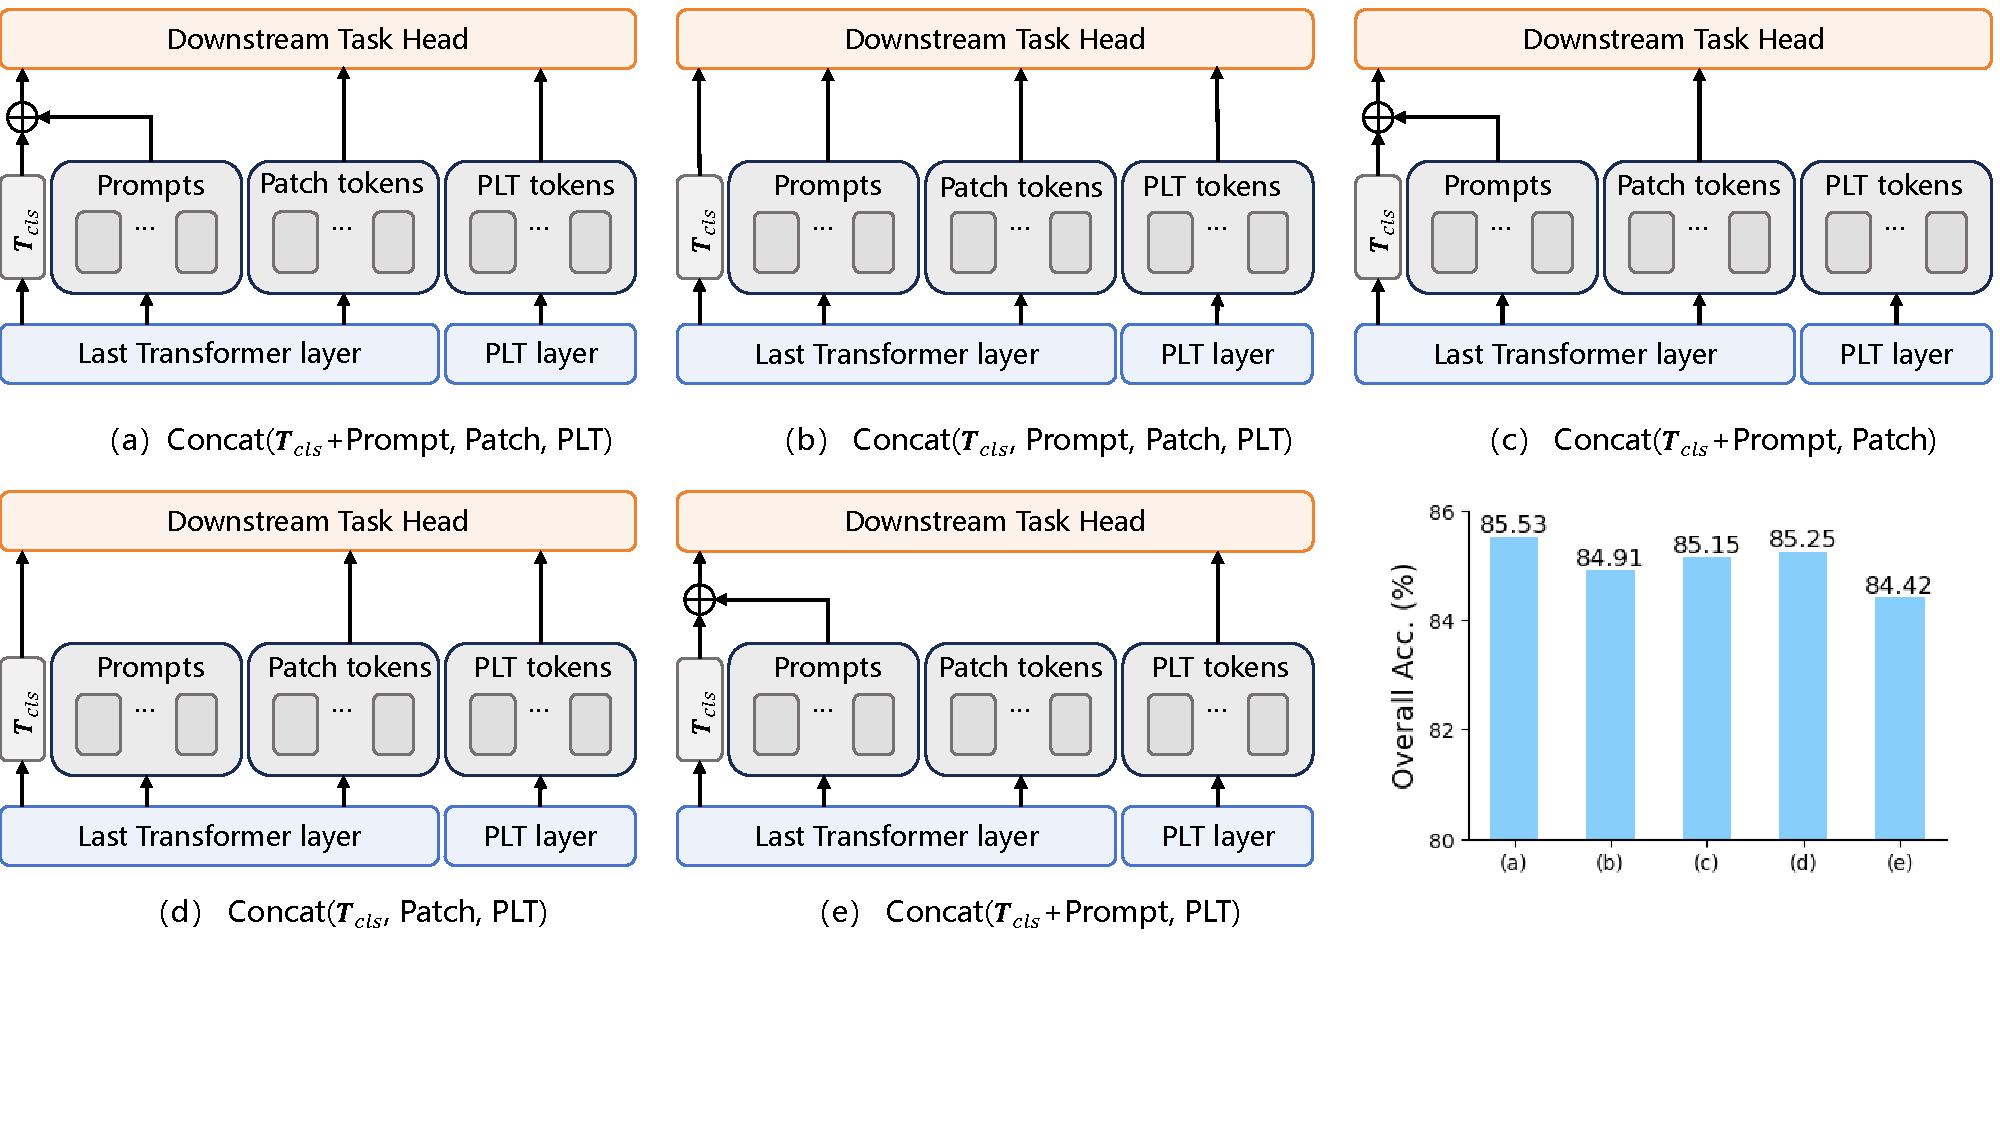
\includegraphics[width=\linewidth]{fig/Effect of different inputs for downstream task head.pdf}
    \caption{Effect of different inputs for downstream classification task head. We conduct experiments on the hardest variant (i.e., PB\_T50\_RS) of ScanObjectNN~\cite{uy2019revisiting} with Point-MAE baseline~\cite{pang2022masked}.}
    \label{fig:whole}
\end{figure*}

\begin{figure*}
    \centering
    \begin{subfigure}{0.24\textwidth}
        \centering
        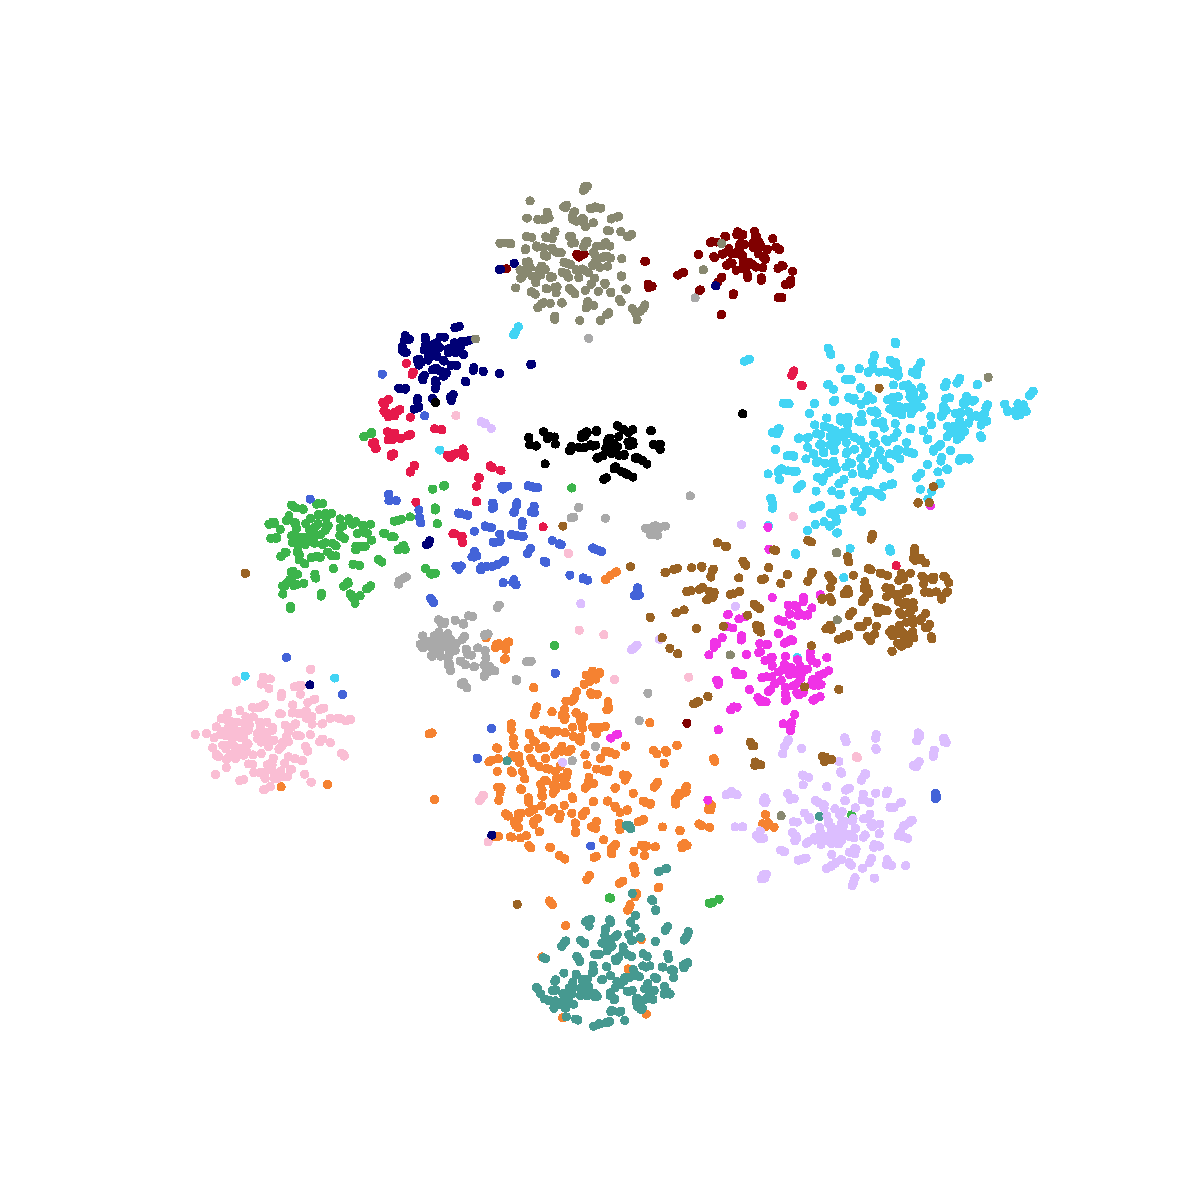
\includegraphics[width=\linewidth]{fig/tsne/point_mae.pdf}
        \caption*{\textbf{\#TP}:22.1M \textbf{\#OA}:85.18}
        \caption{Full fine-tuning}
        \label{fig:sub1}
    \end{subfigure}
    \hfill
    \begin{subfigure}{0.24\textwidth}
        \centering
        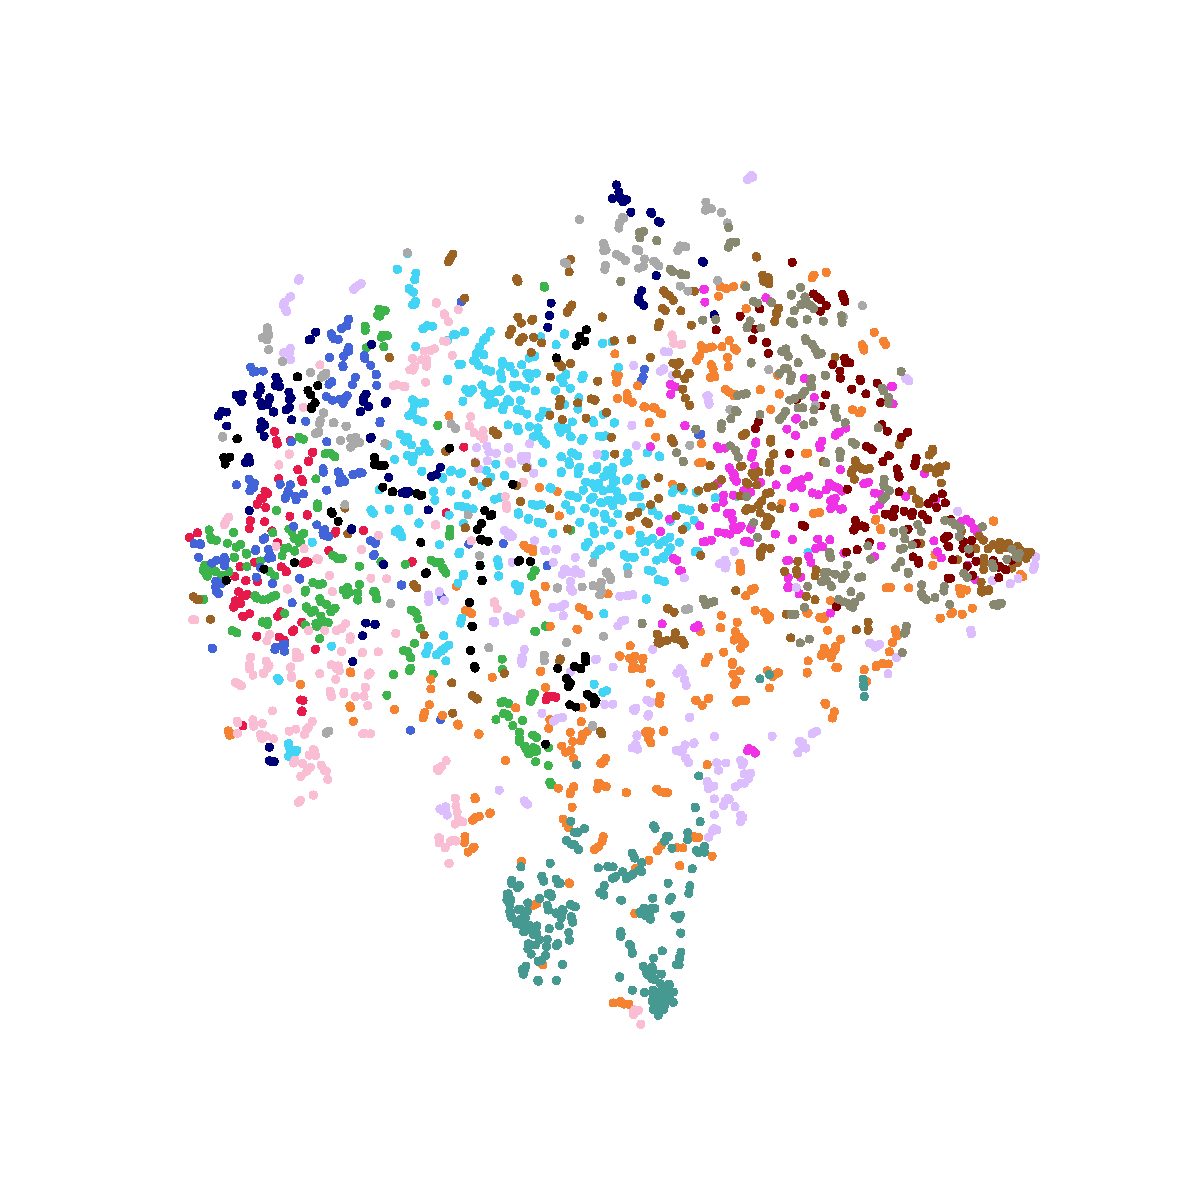
\includegraphics[width=\linewidth]{fig/tsne/LP.pdf}
        \caption*{\textbf{\#TP}:0.3M \textbf{\#OA}:75.99}
        \caption{Linear Probing}
        \label{fig:sub2}
    \end{subfigure}
    \hfill
    \begin{subfigure}{0.24\textwidth}
        \centering
        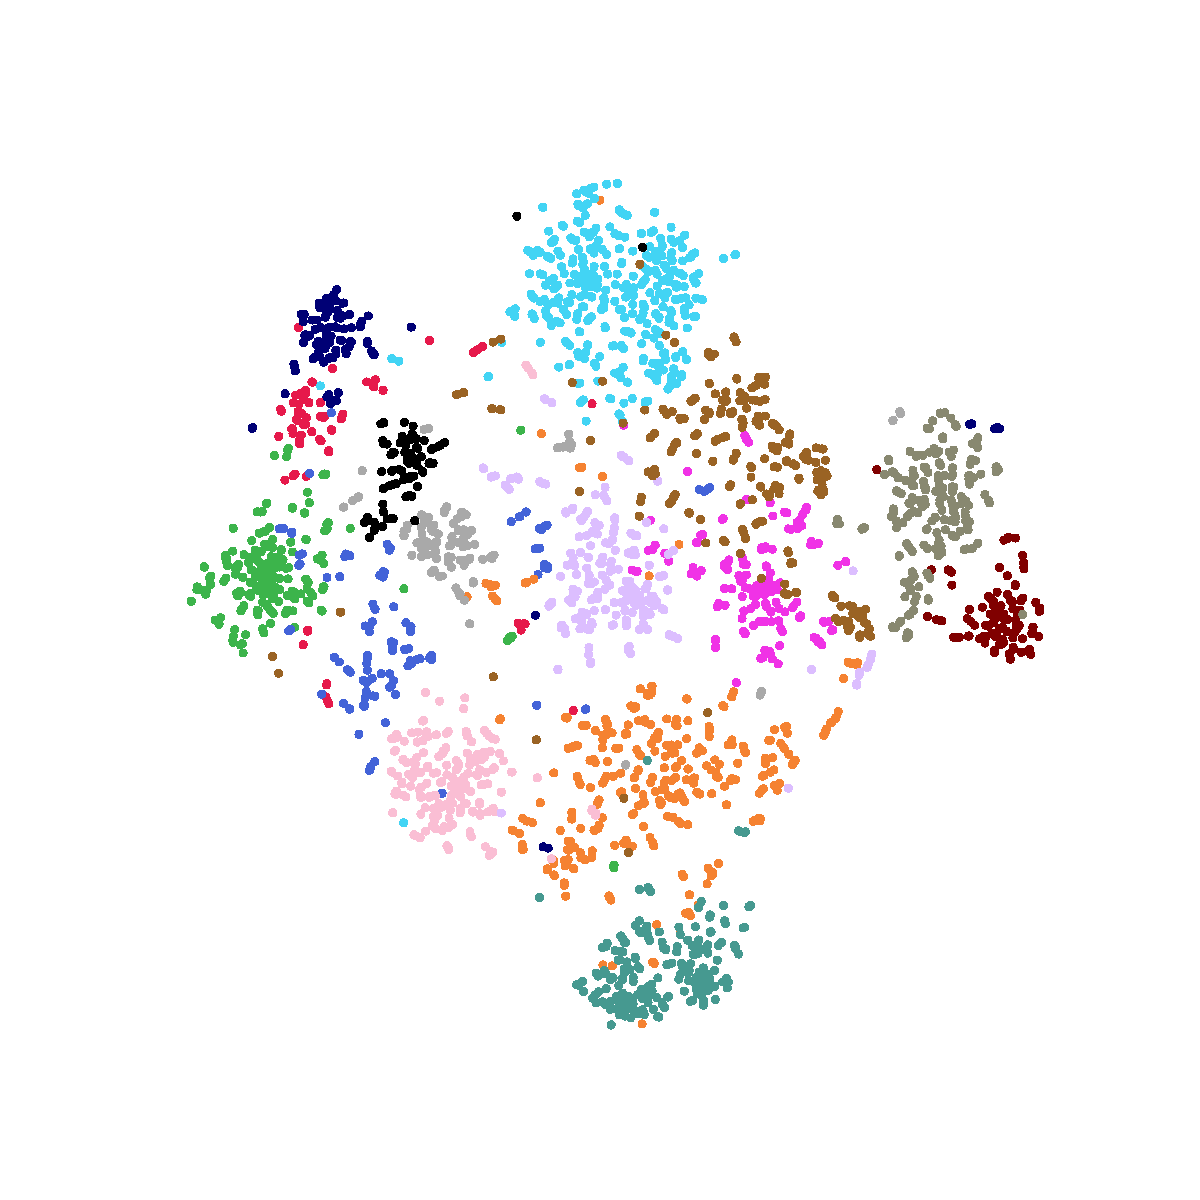
\includegraphics[width=\linewidth]{fig/tsne/idpt.pdf}
        \caption*{\textbf{\#TP}:1.7M \textbf{\#OA}:84.94}
        \caption{IDPT}
        \label{fig:sub3}
    \end{subfigure}
    \hfill
    \begin{subfigure}{0.24\textwidth}
        \centering
        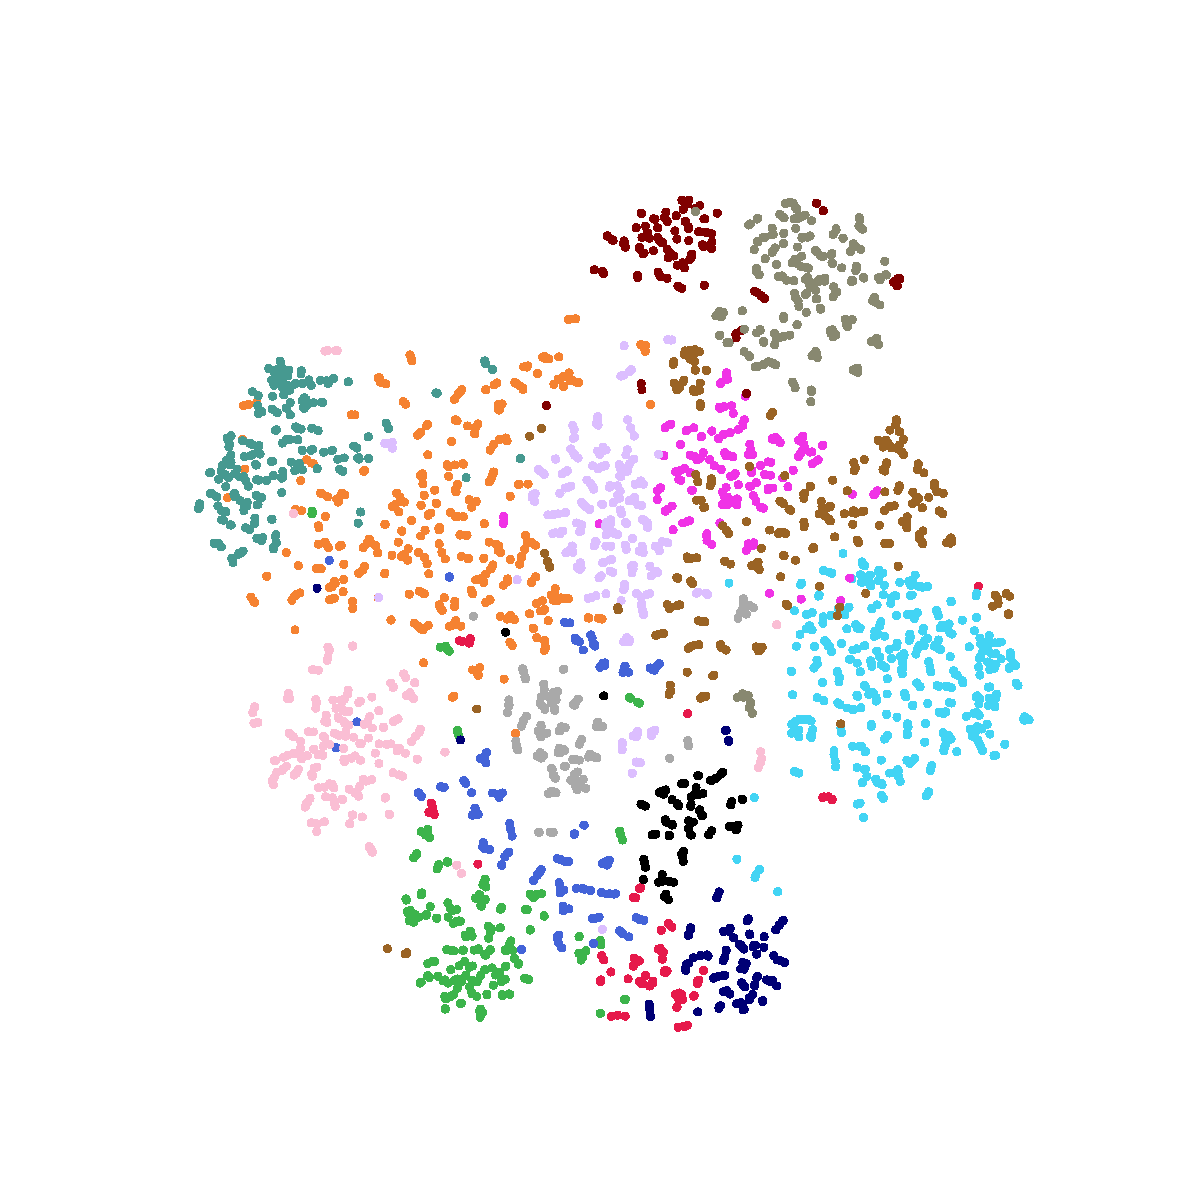
\includegraphics[width=\linewidth]{fig/tsne/dapt.pdf}
        \caption*{\textbf{\#TP}:1.1M \textbf{\#OA}:85.08}
        \caption{DAPT}
        \label{fig:sub4}
    \end{subfigure}
    \hfill
    \begin{subfigure}{0.24\textwidth}
        \centering
        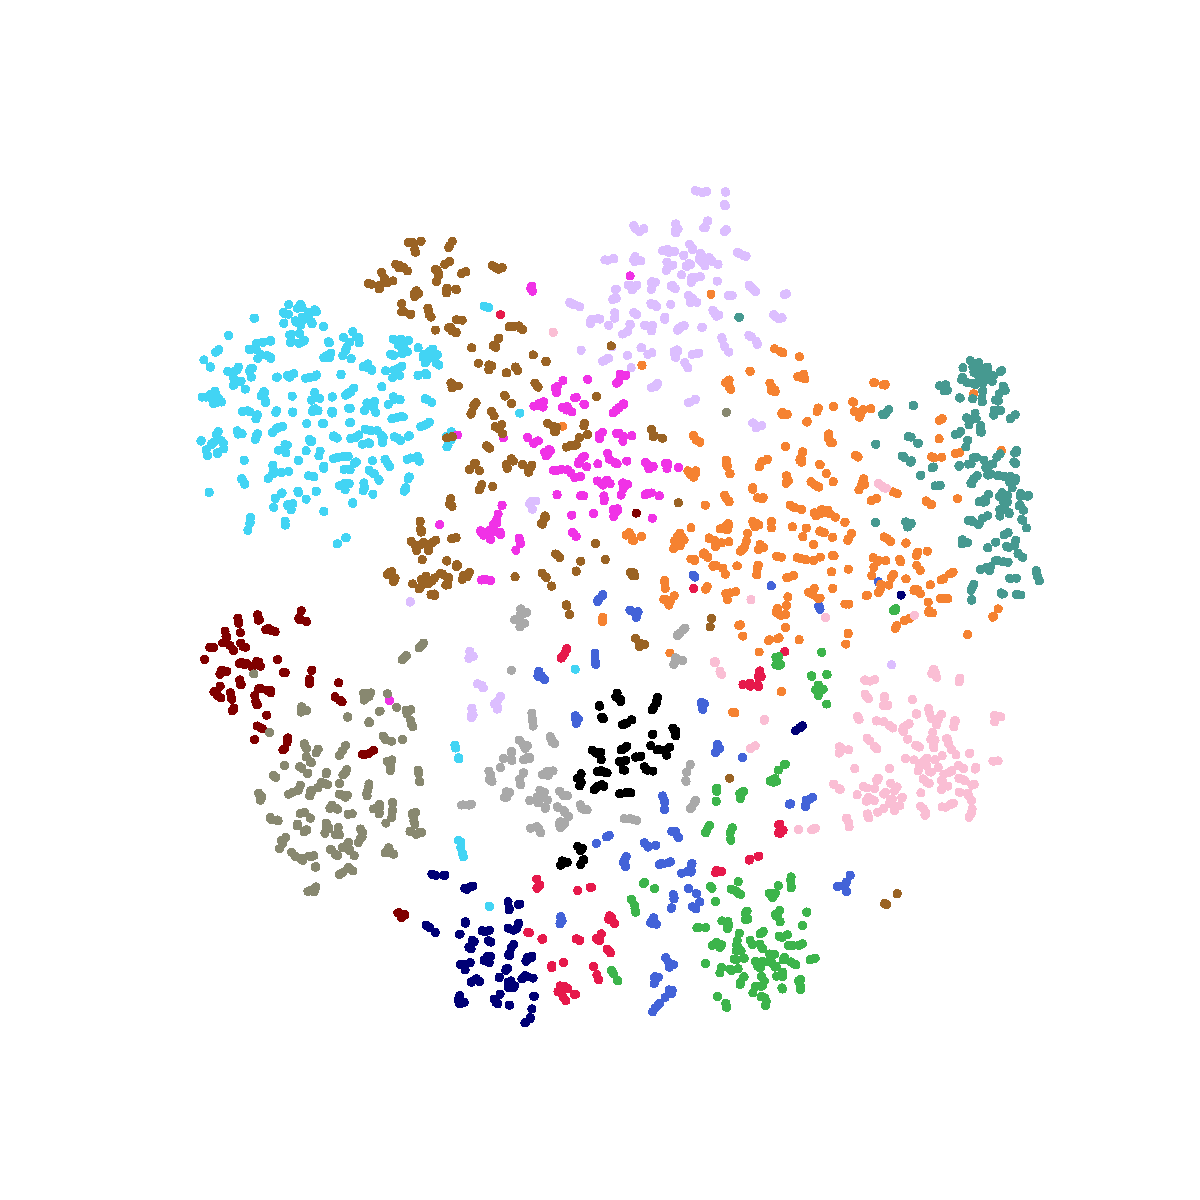
\includegraphics[width=\linewidth]{fig/tsne/pointgst.pdf}
        \caption*{\textbf{\#TP}:0.6M \textbf{\#OA}:85.29}
        \caption{PointGST}
        \label{fig:sub5}
    \end{subfigure}
    \hfill
    \begin{subfigure}{0.24\textwidth}
        \centering
        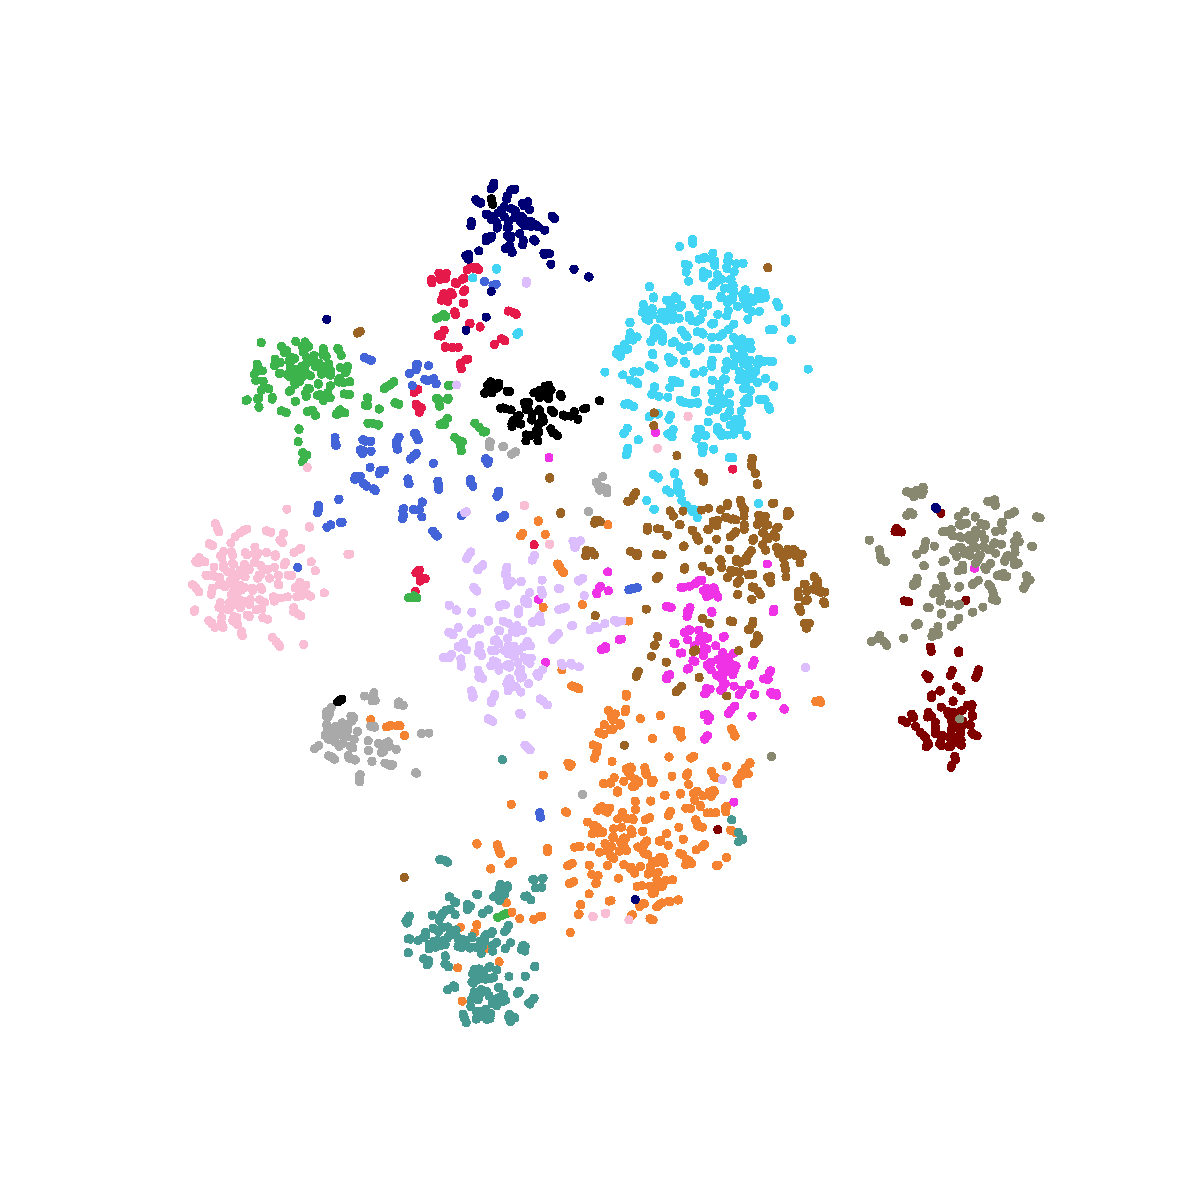
\includegraphics[width=\linewidth]{fig/tsne/PPT.pdf}
        \caption*{\textbf{\#TP}:1.1M \textbf{\#OA}:84.91}
        \caption{PPT}
        \label{fig:sub6}
    \end{subfigure}
    \hfill
    \begin{subfigure}{0.24\textwidth}
        \centering
        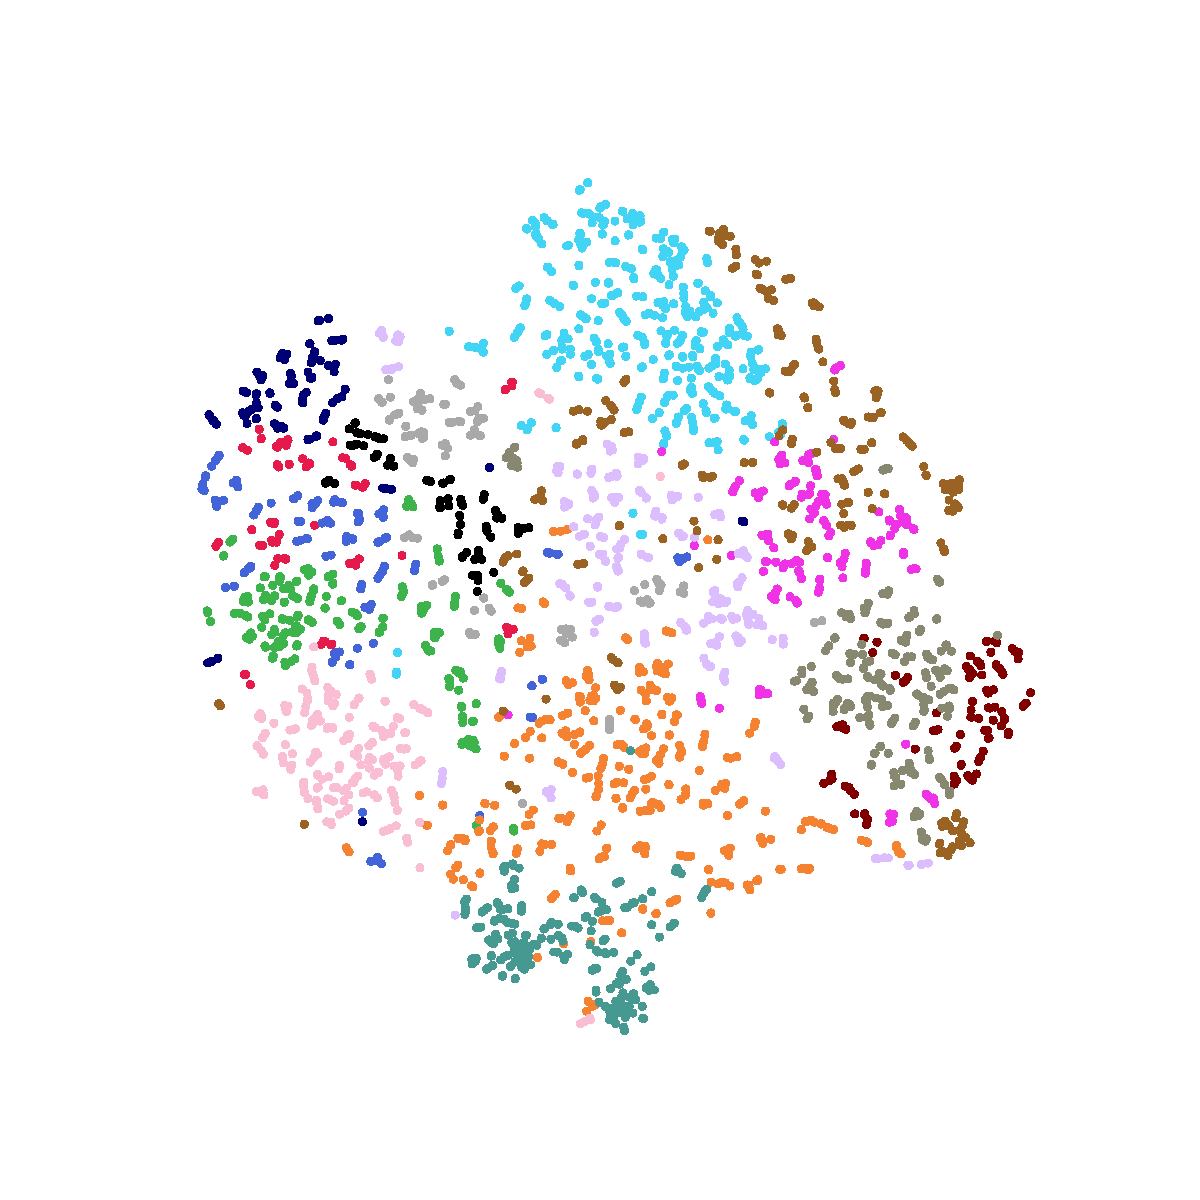
\includegraphics[width=\linewidth]{fig/tsne/LST.pdf}
        \caption*{\textbf{\#TP}:0.8M \textbf{\#OA}:82.75}
        \caption{LST}
        \label{fig:sub7}
    \end{subfigure}
    \hfill
    \begin{subfigure}{0.24\textwidth}
        \centering
        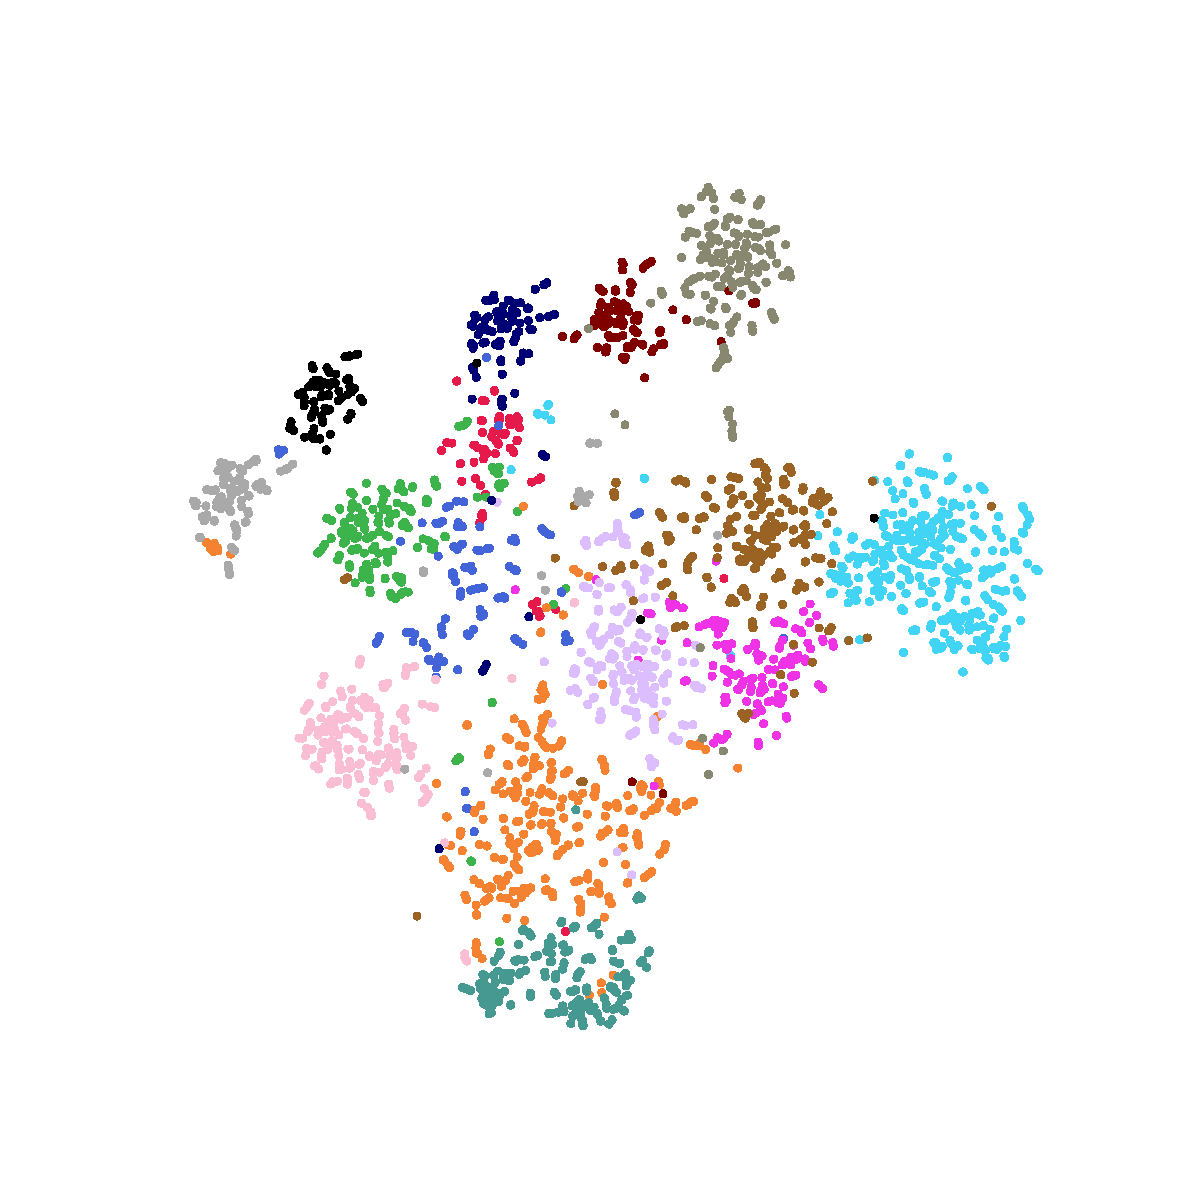
\includegraphics[width=\linewidth]{fig/tsne/point_ladder.pdf}
        \caption*{\textbf{\#TP}:0.6M \textbf{\#OA}:85.53}
        \caption{PLT (Ours)}
        \label{fig:sub8}
    \end{subfigure}
    \caption{The visualization of the t-SNE~\cite{van2008visualizing} from the test sets of ScanObjectNN~\cite{uy2019revisiting} (PB\_T50\_RS) by using a pre-trained PointMAE~\cite{pang2022masked} with various fine-tuning strategies. We extract the final classification features from the top linear layer for t-SNE visualizations.}
    \label{fig:tsne1}
\end{figure*}

\begin{figure*}[htbp]
    \centering

    % 第一行左侧的竖排标签
    \begin{minipage}{0.1\textwidth}
        \centering
        {airplane}
        % \rotatebox{90}{14}
    \end{minipage}
    \hfill
    % 第一行图片
    \begin{minipage}{0.25\textwidth}
        \centering
        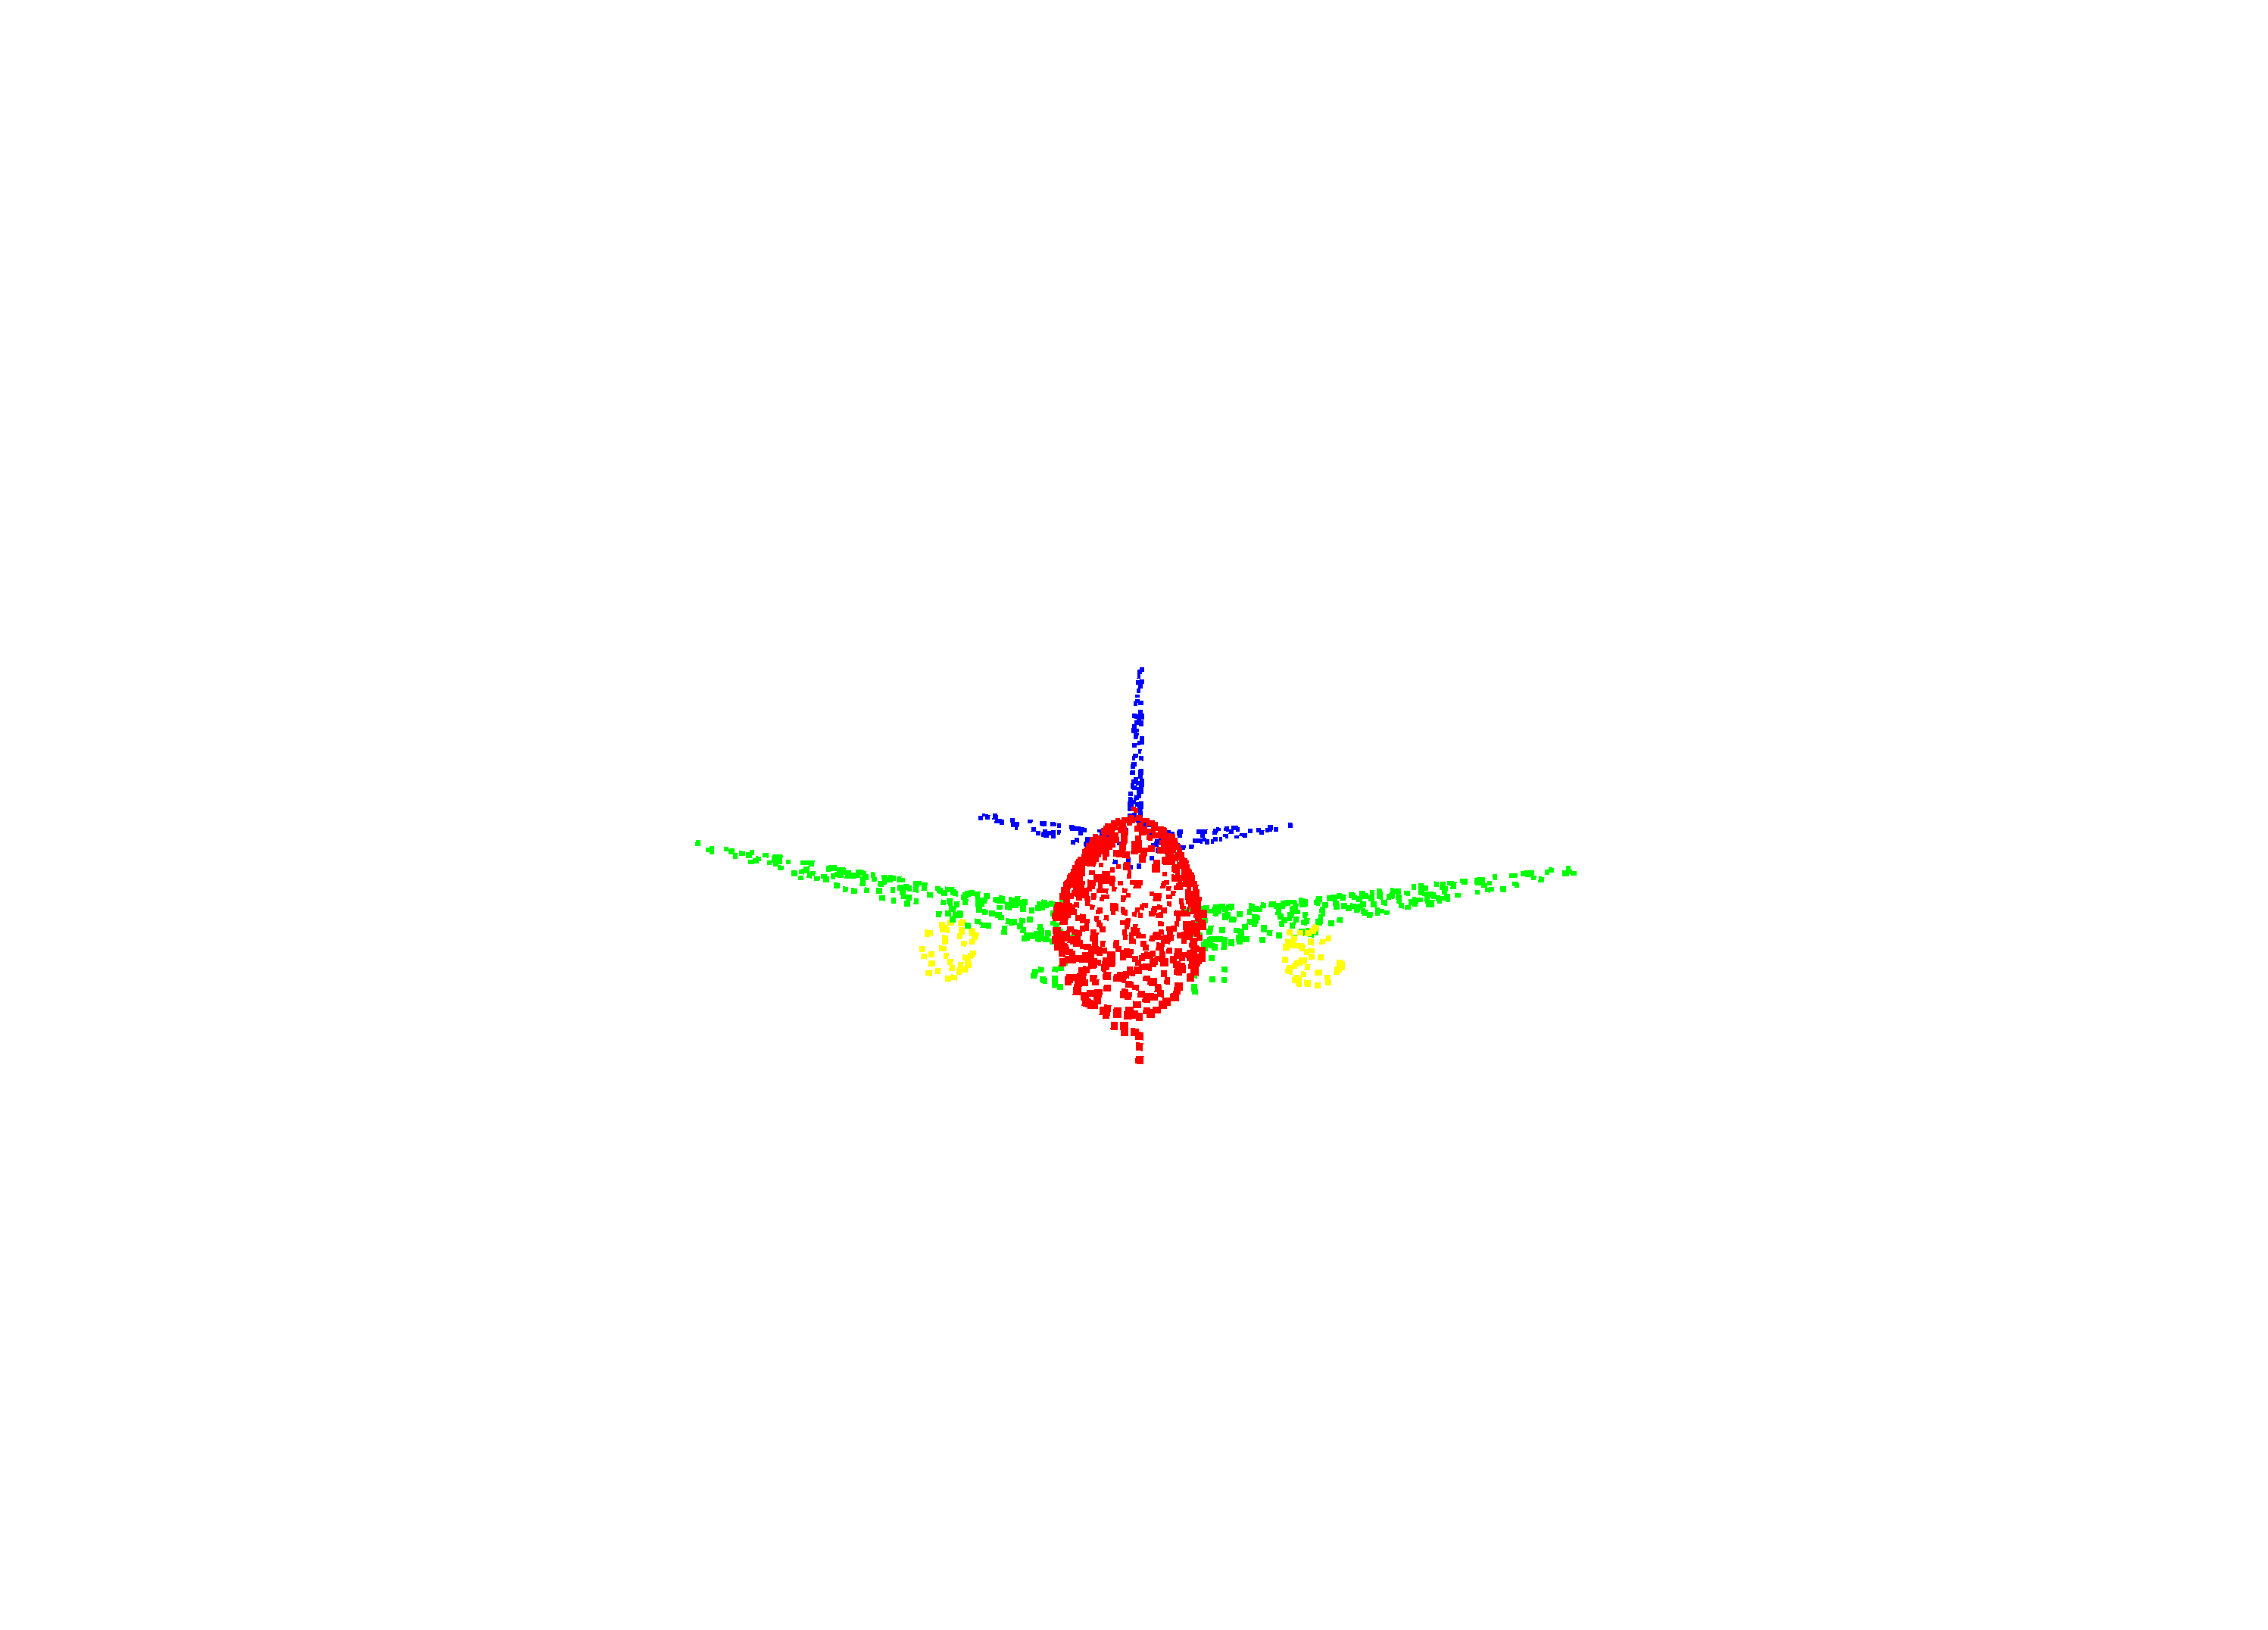
\includegraphics[width=\textwidth]{fig/supplement/part_segmentation/airplane/airplane00.pdf} % 替换为你的图片路径
    \end{minipage}
    \hfill
    \begin{minipage}{0.25\textwidth}
        \centering
        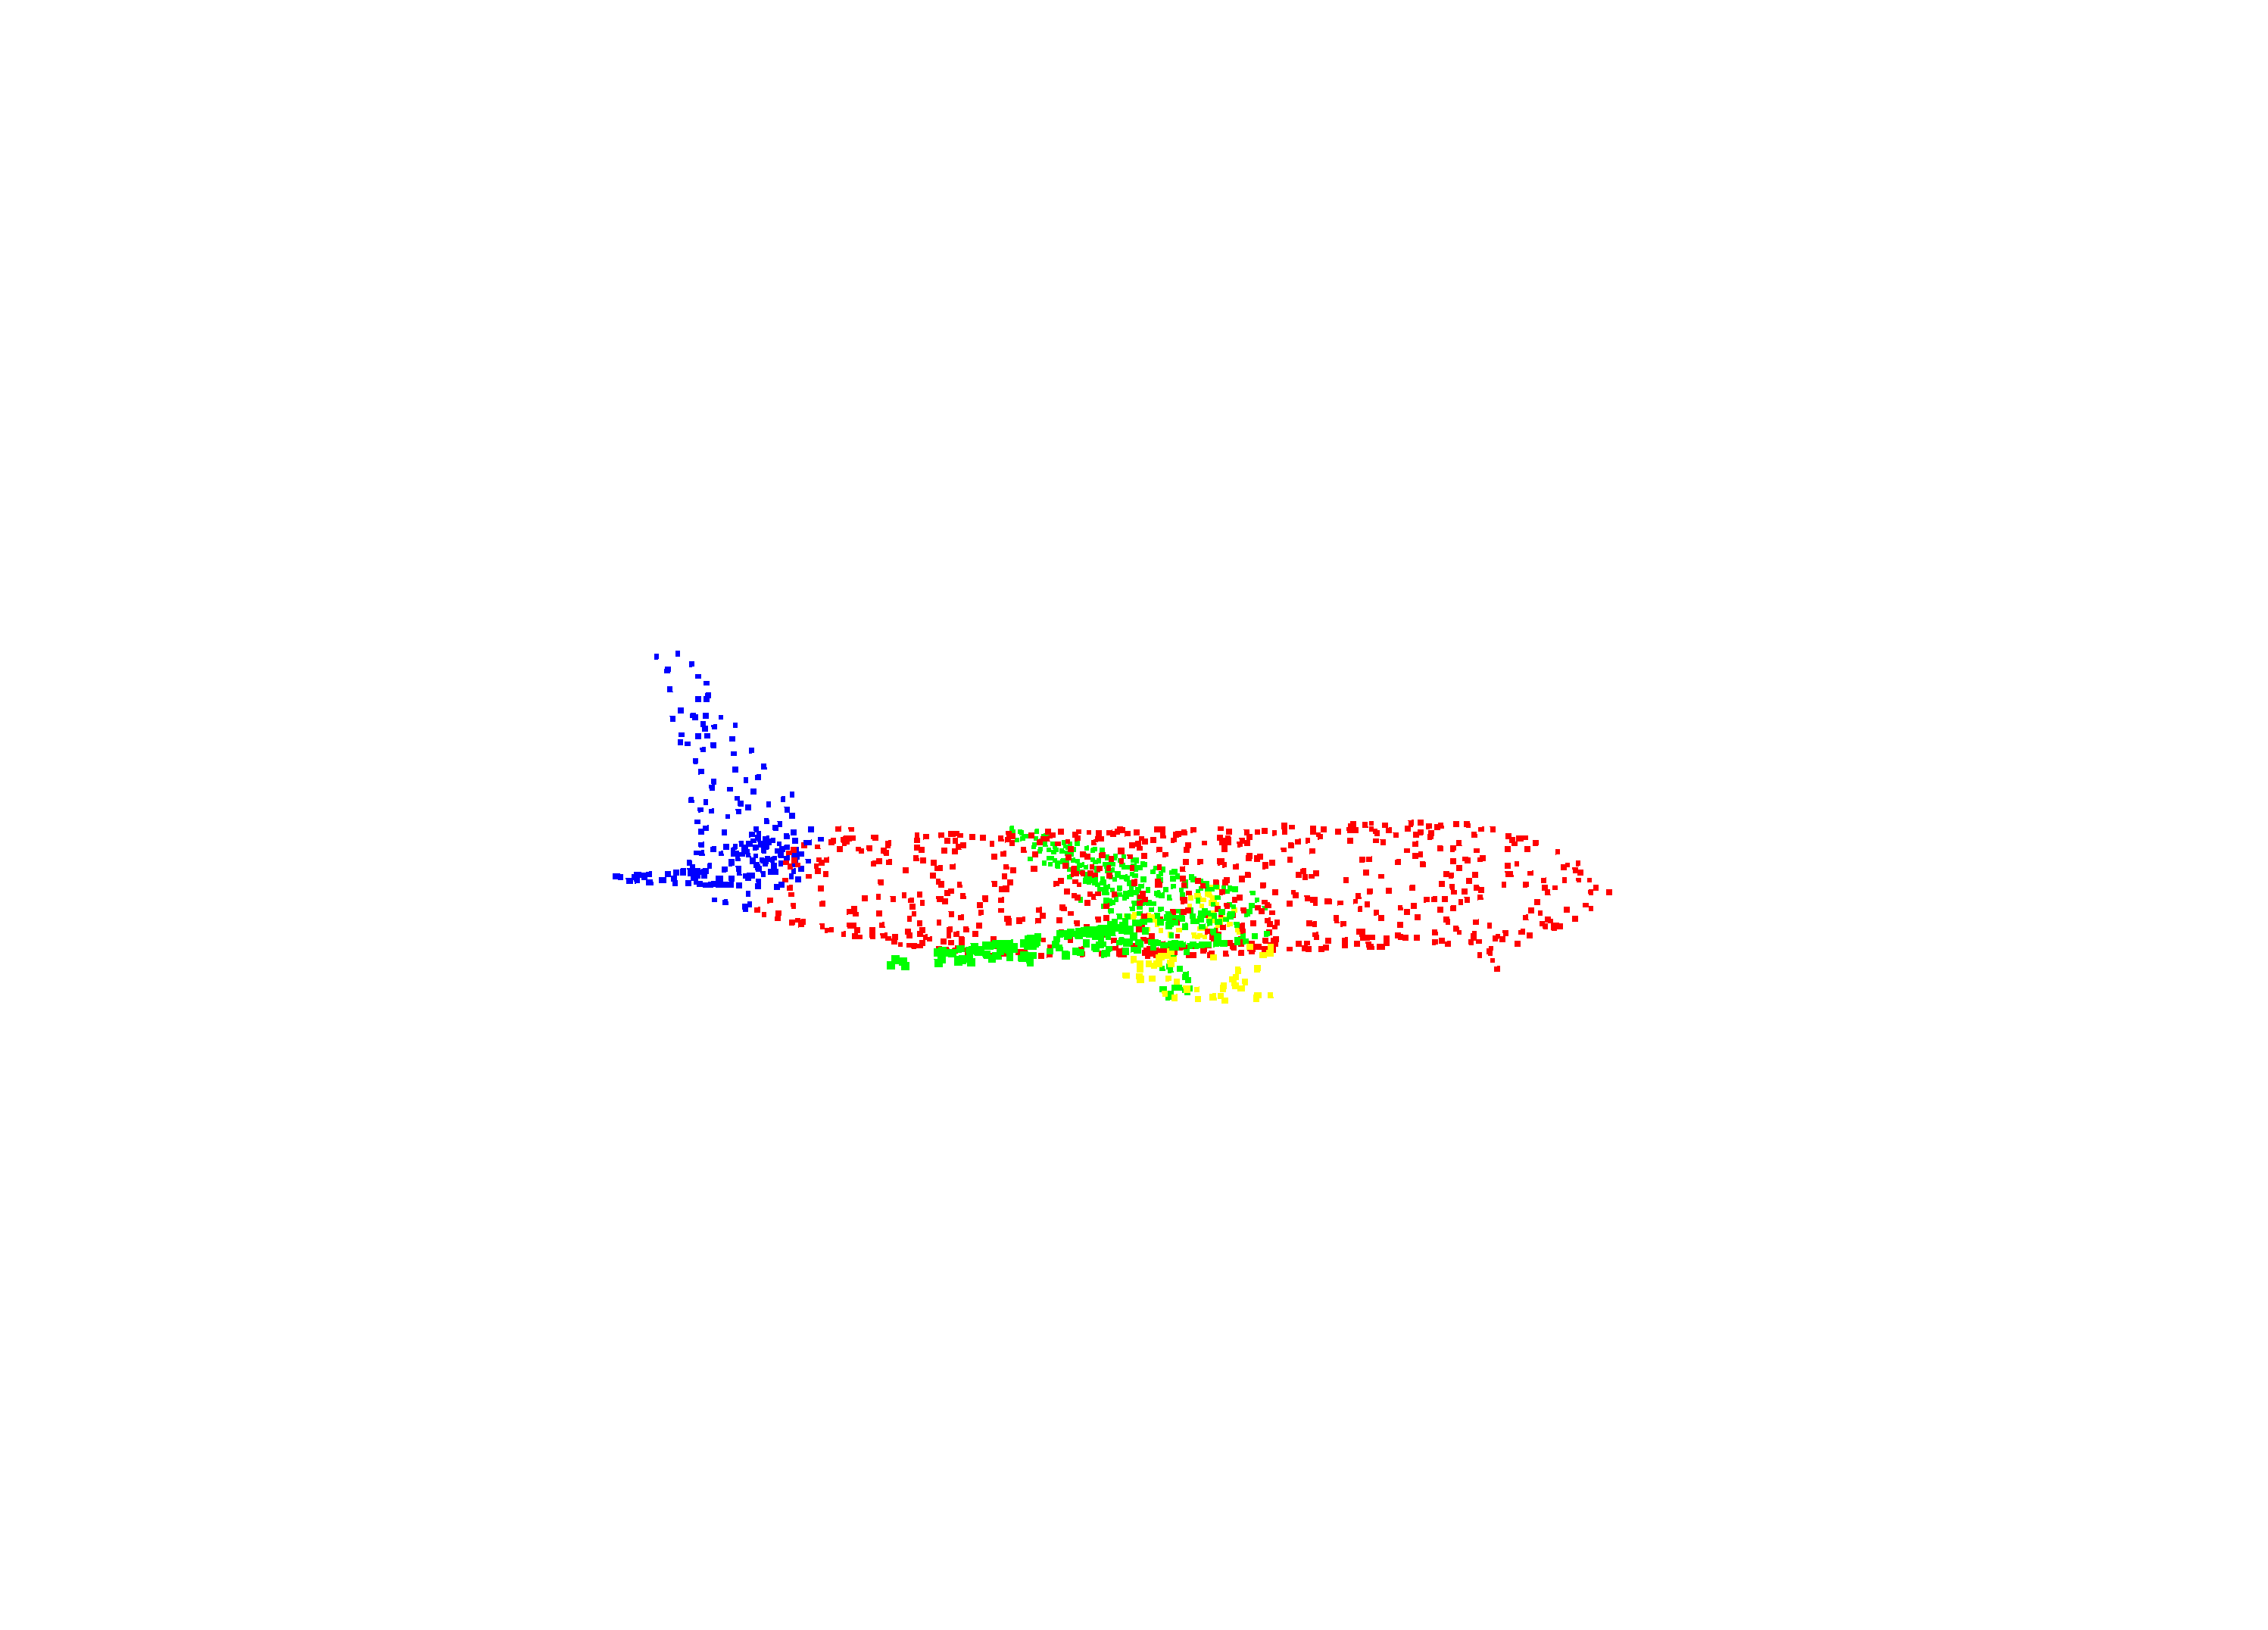
\includegraphics[width=\textwidth]{fig/supplement/part_segmentation/airplane/airplane01.pdf}
    \end{minipage}
    \hfill
    \begin{minipage}{0.25\textwidth}
        \centering
        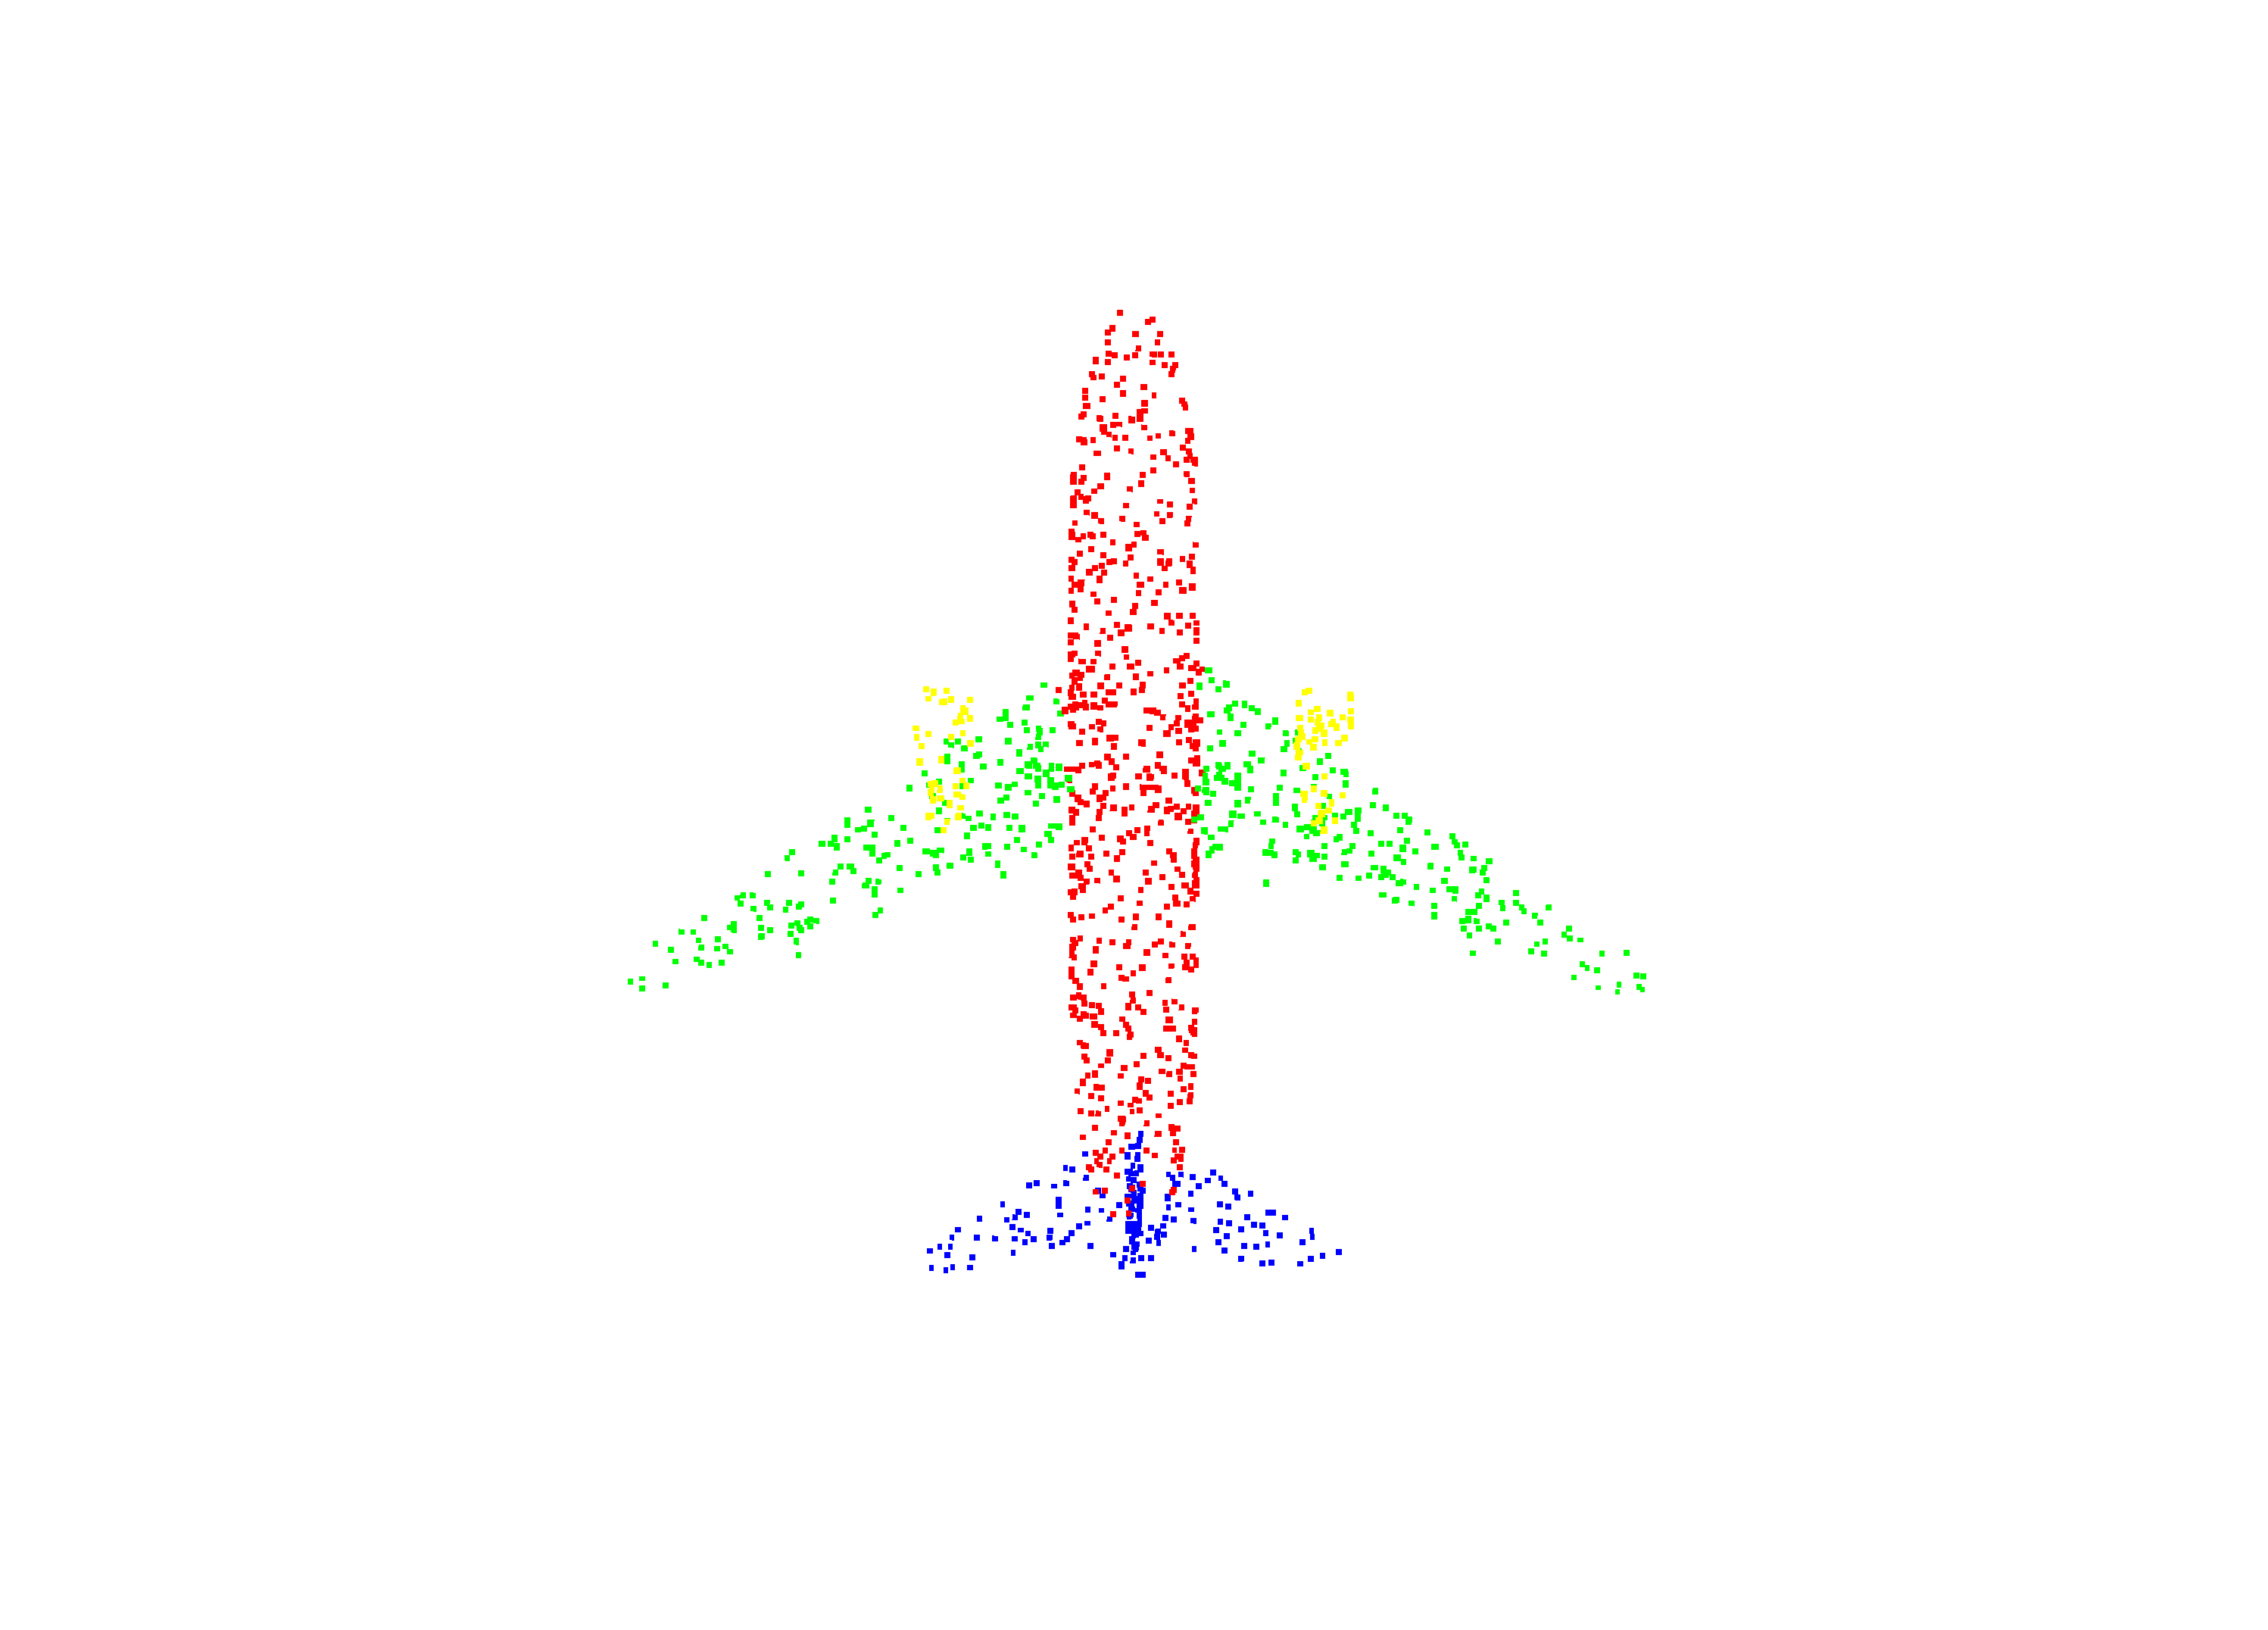
\includegraphics[width=\textwidth]{fig/supplement/part_segmentation/airplane/airplane02.pdf}
    \end{minipage}
    \hfill

    % 换行
    \vspace{0.5em}

    % 第二行左侧的竖排标签
    \begin{minipage}{0.1\textwidth}
        \centering
        {chair}
    \end{minipage}
    \hfill
    % 第二行图片
    \begin{minipage}{0.25\textwidth}
        \centering
        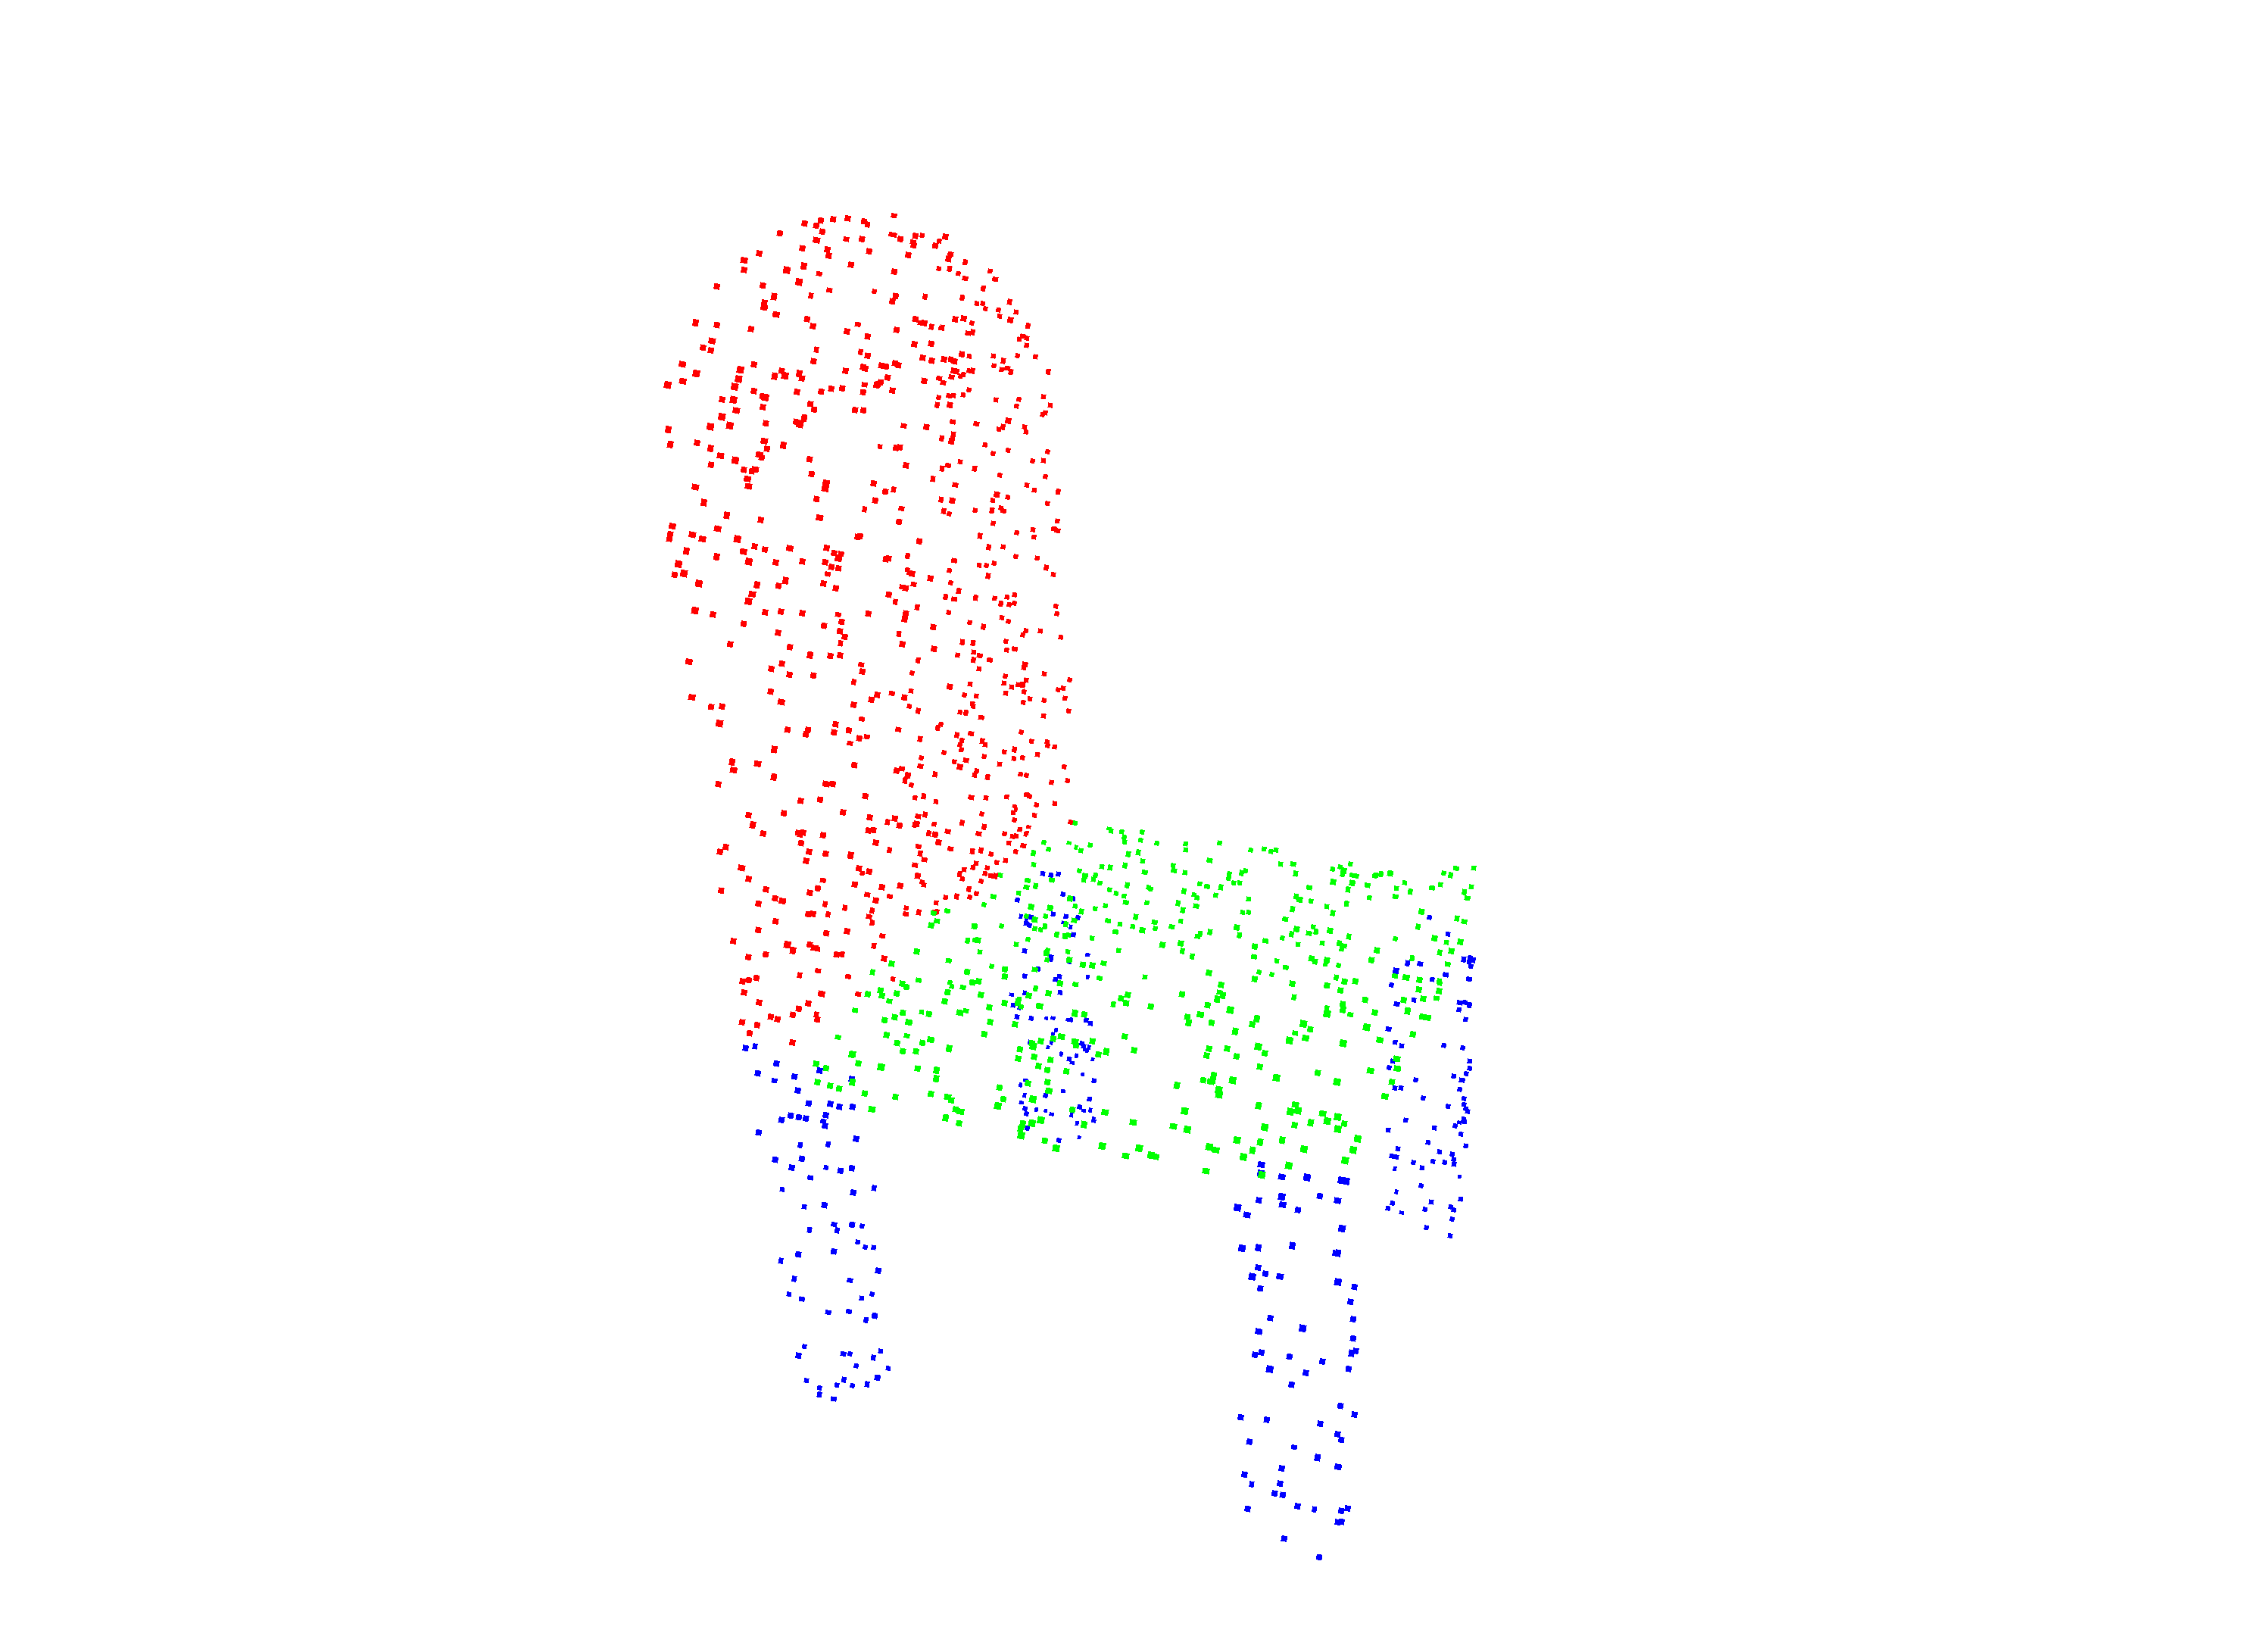
\includegraphics[width=\textwidth]{fig/supplement/part_segmentation/chair/chair00.pdf}
    \end{minipage}
    \hfill
    \begin{minipage}{0.25\textwidth}
        \centering
        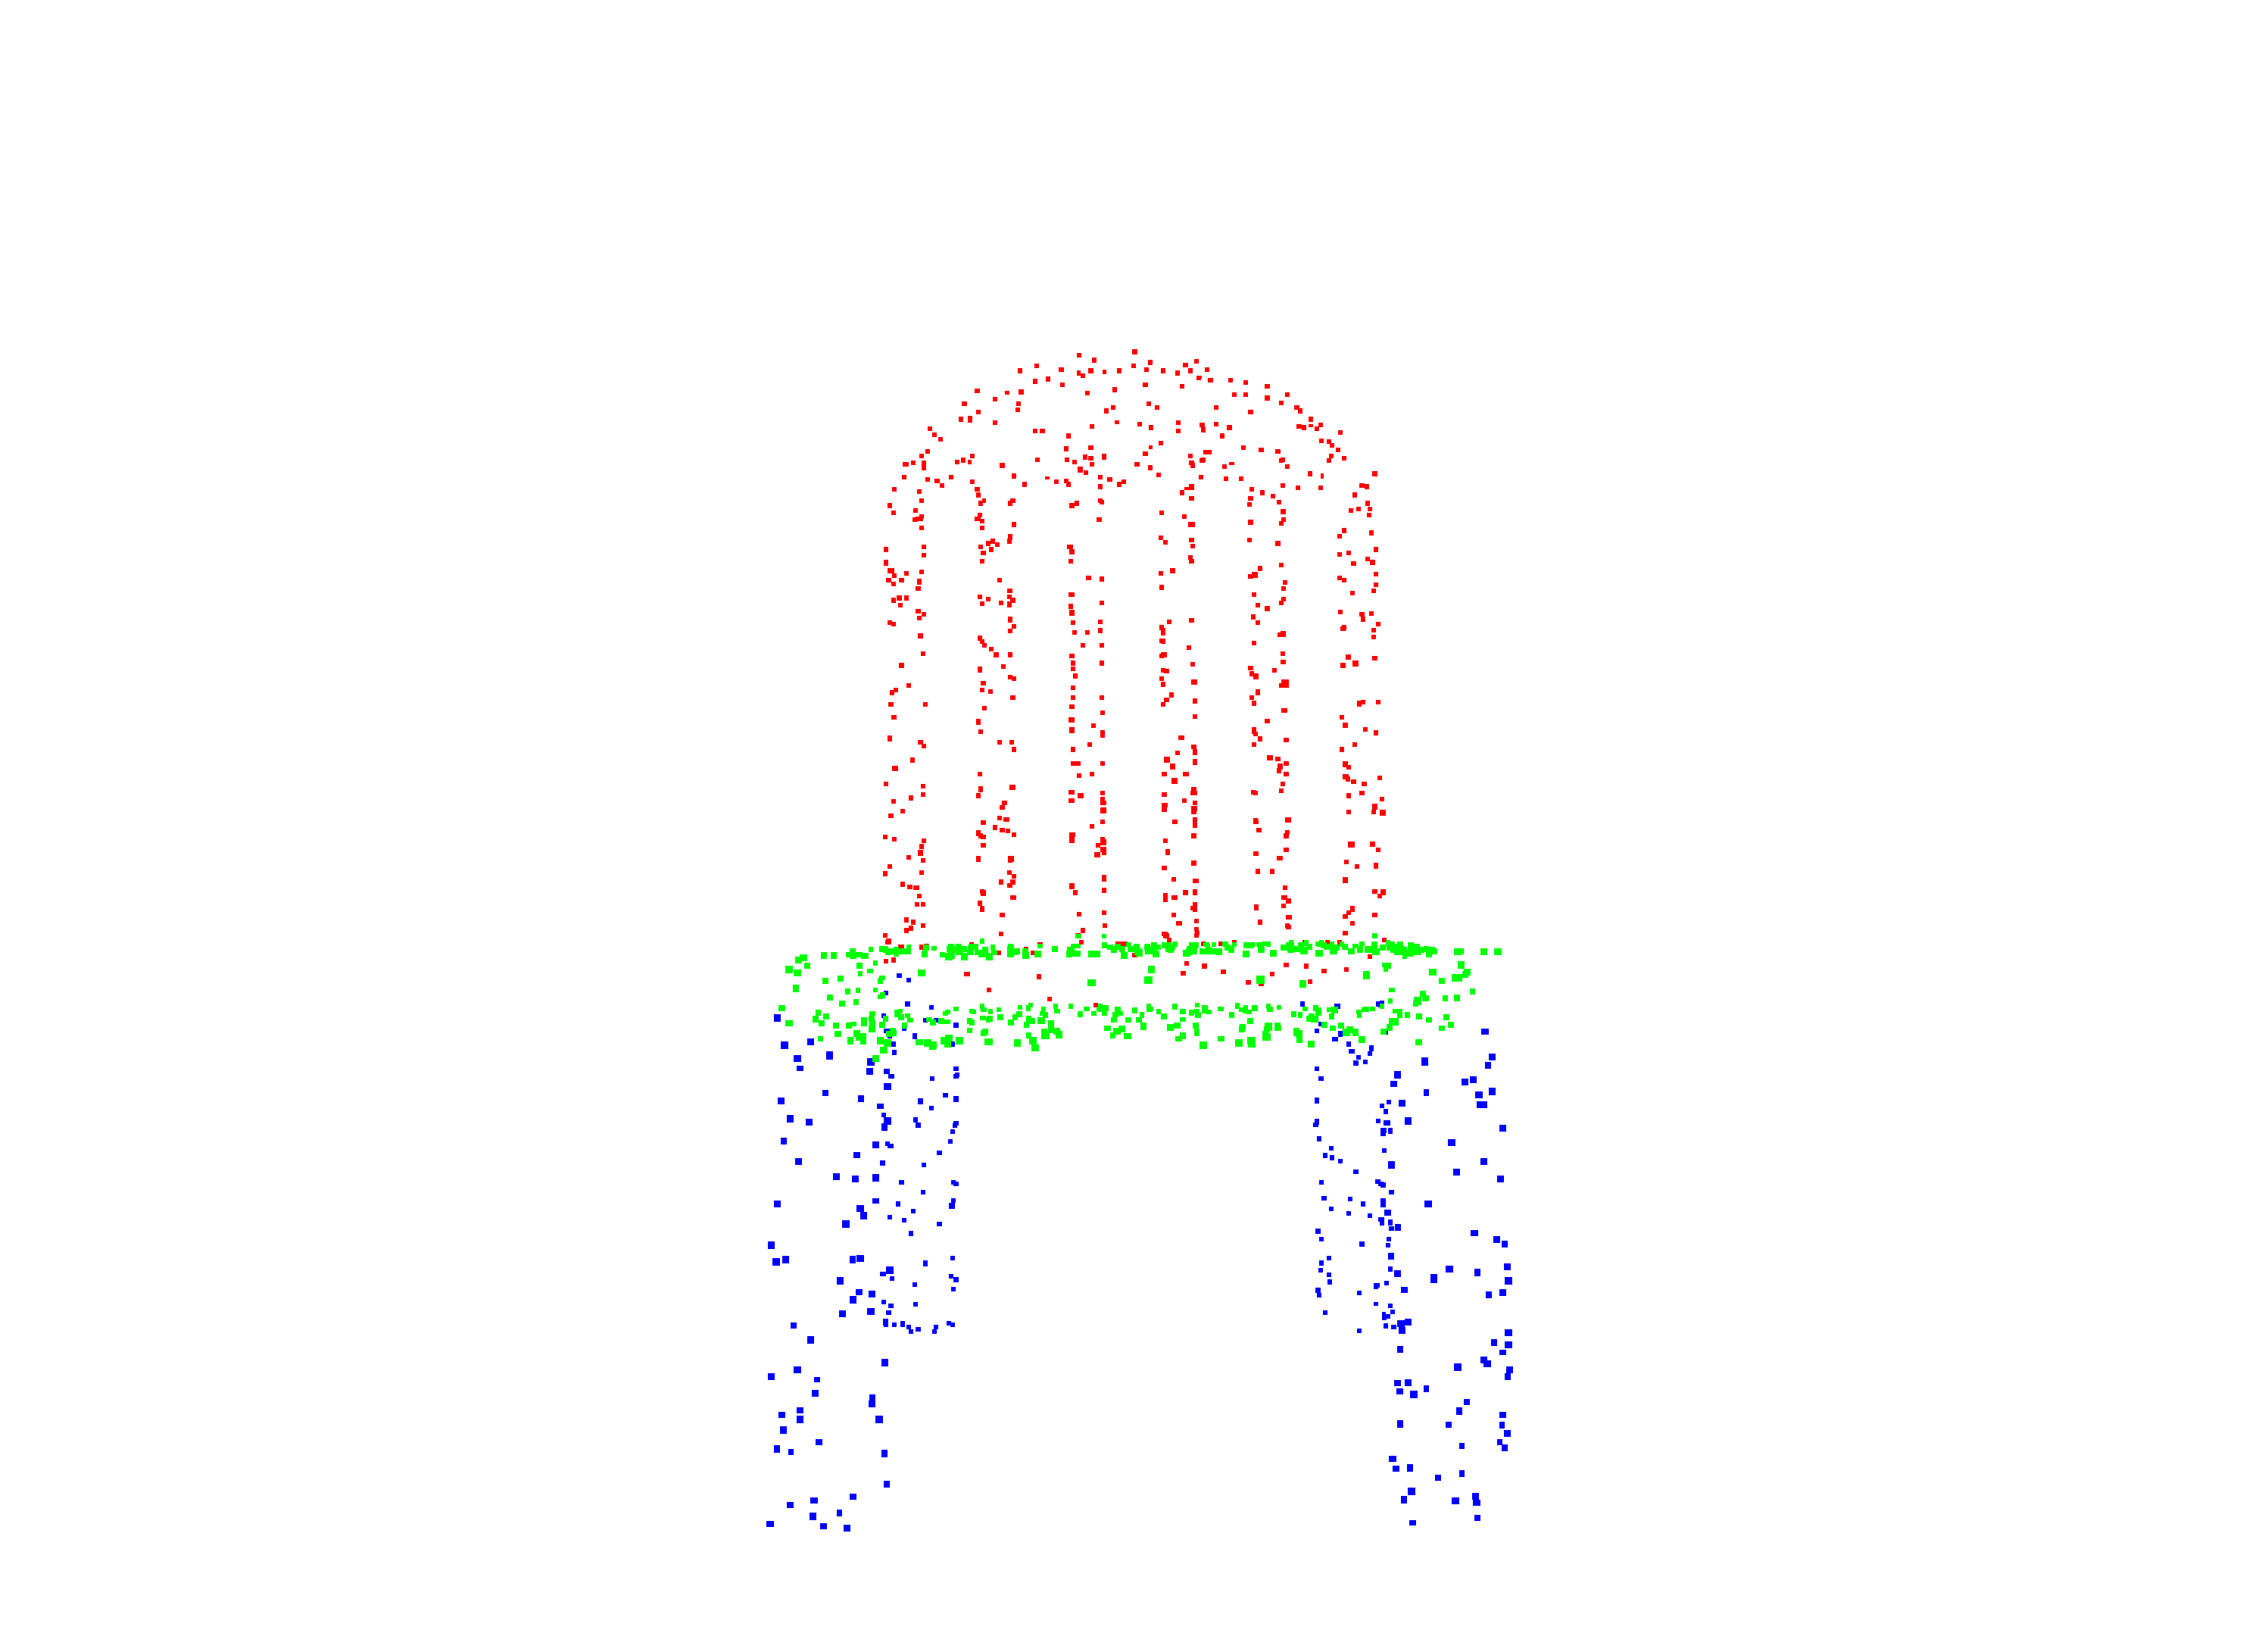
\includegraphics[width=\textwidth]{fig/supplement/part_segmentation/chair/chair01.pdf}
    \end{minipage}
    \hfill
    \begin{minipage}{0.25\textwidth}
        \centering
        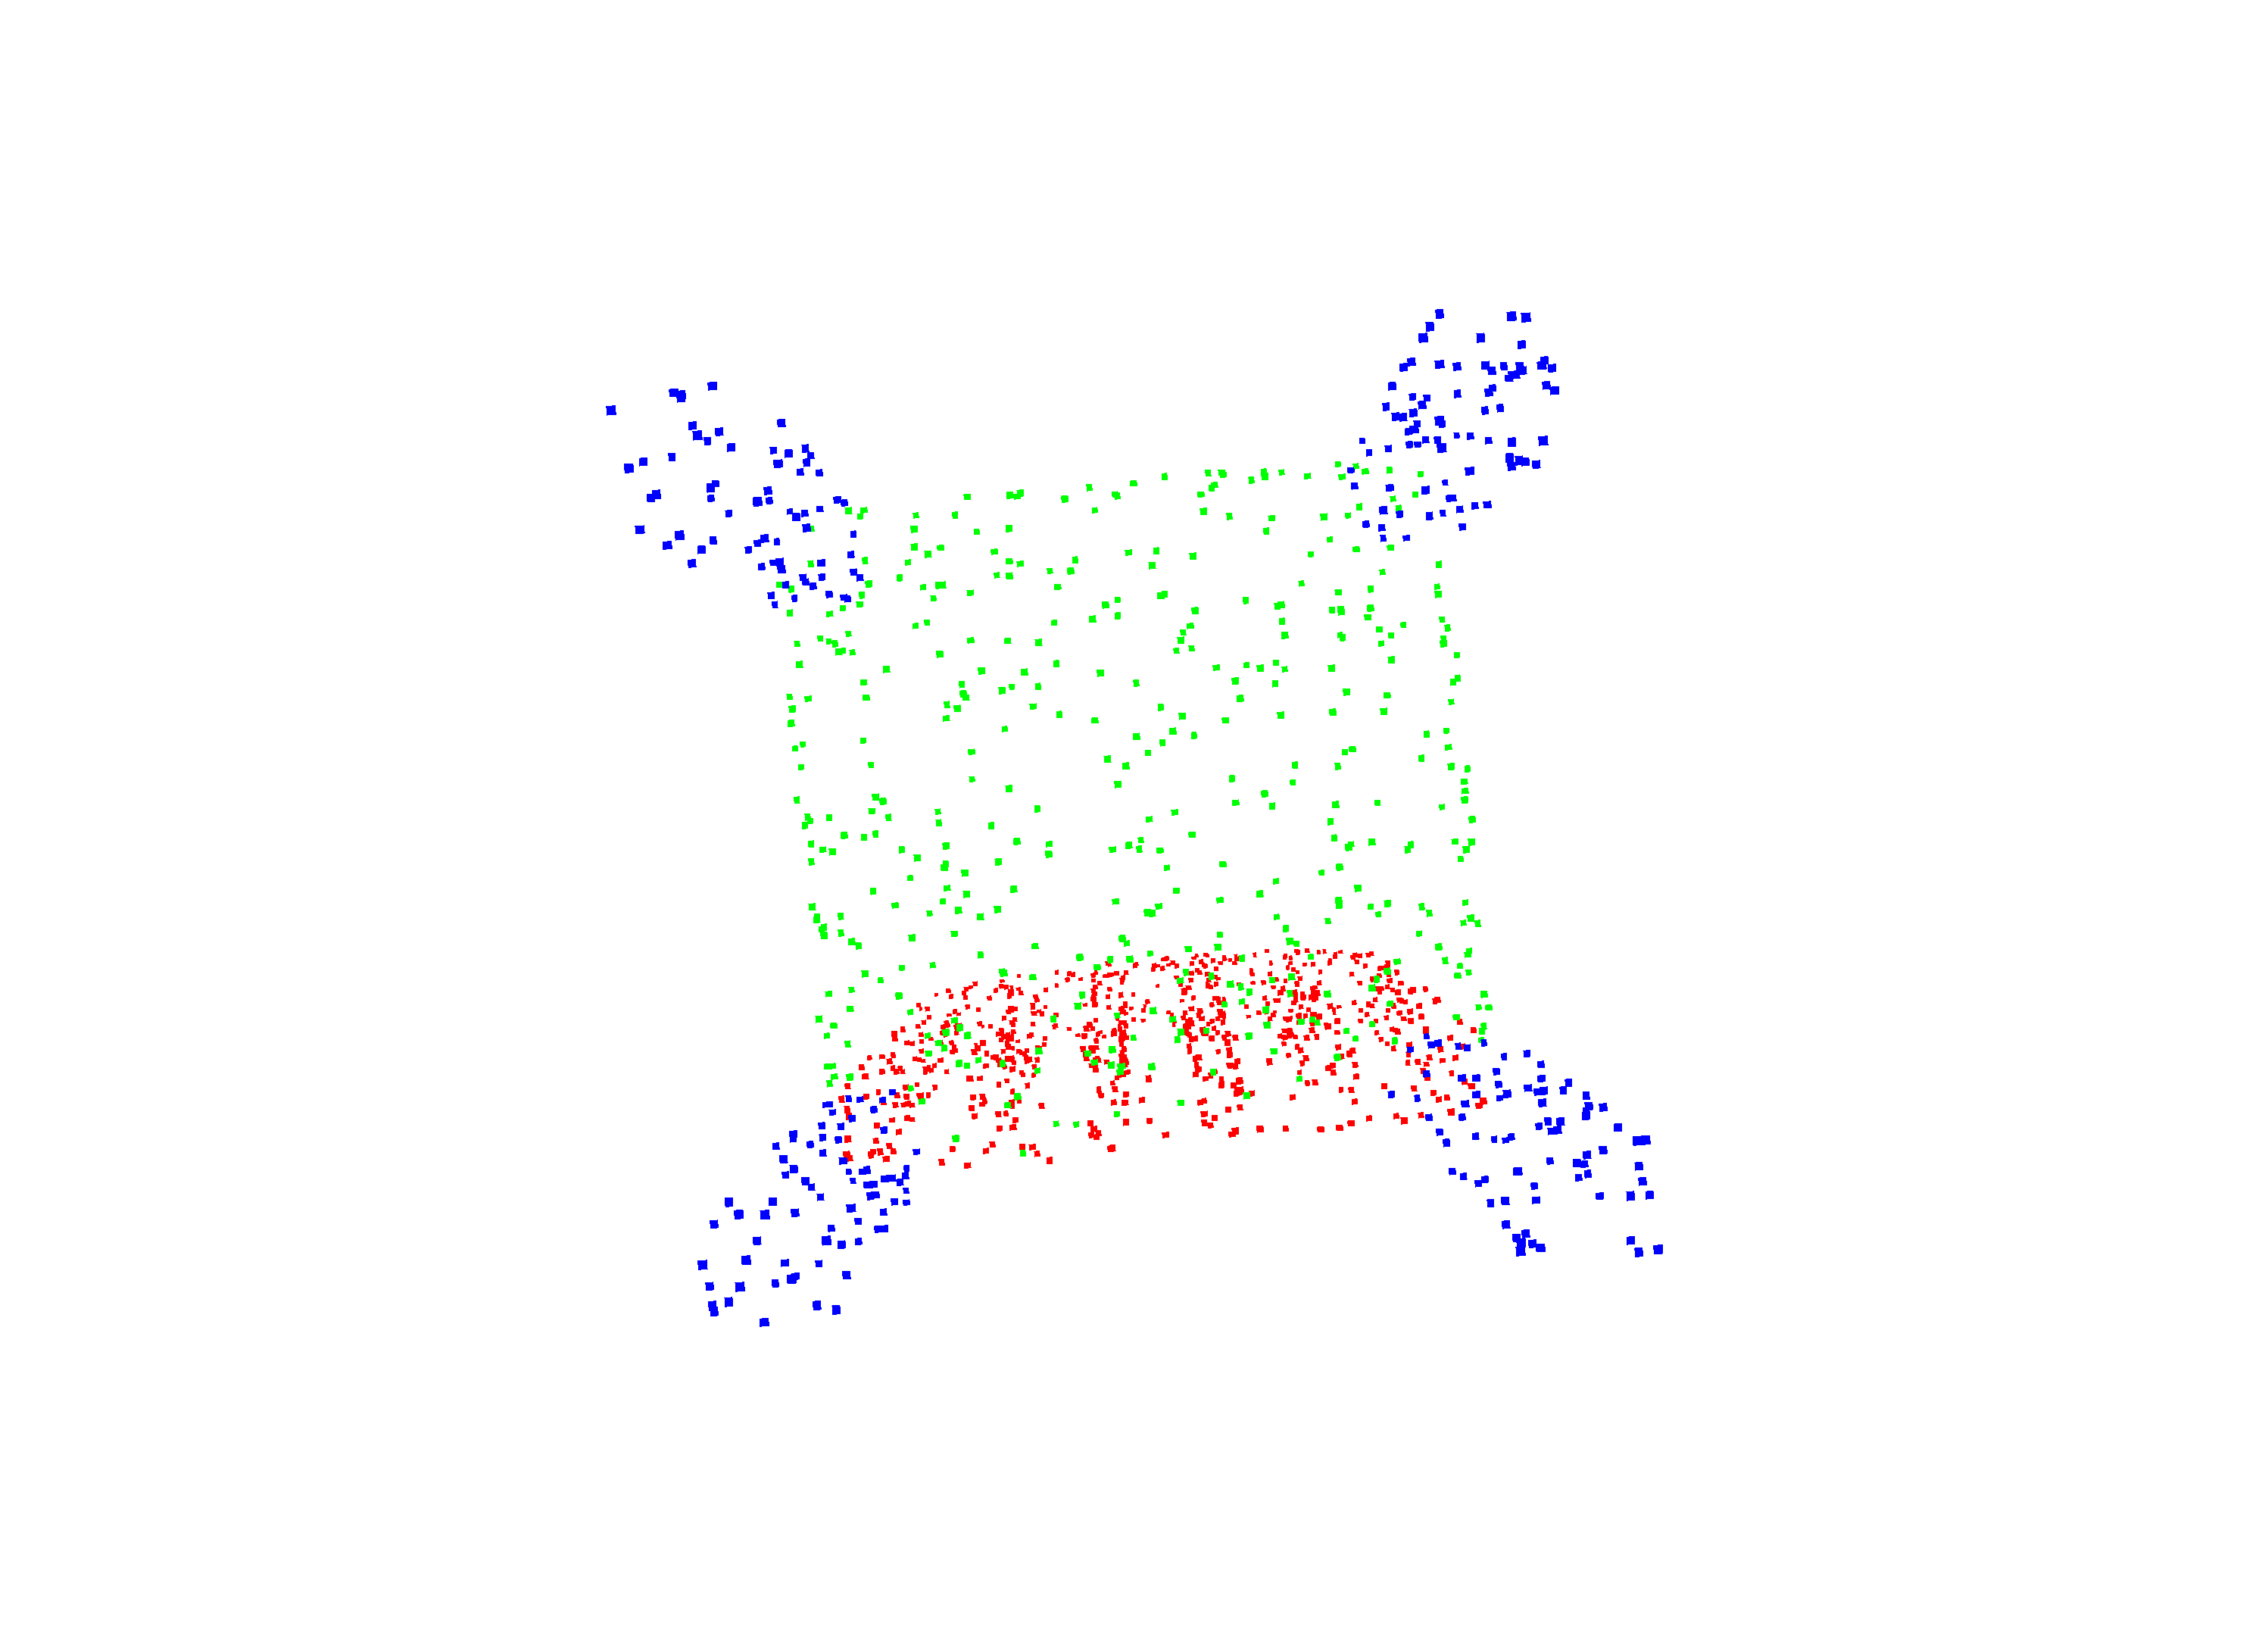
\includegraphics[width=\textwidth]{fig/supplement/part_segmentation/chair/chair02.pdf}
    \end{minipage}
    \hfill

    % 换行
    \vspace{0.5em}

    % 第三行左侧的竖排标签
    \begin{minipage}{0.1\textwidth}
        \centering
        {lamp}
    \end{minipage}
    \hfill
    % 第三行图片
    \begin{minipage}{0.25\textwidth}
        \centering
        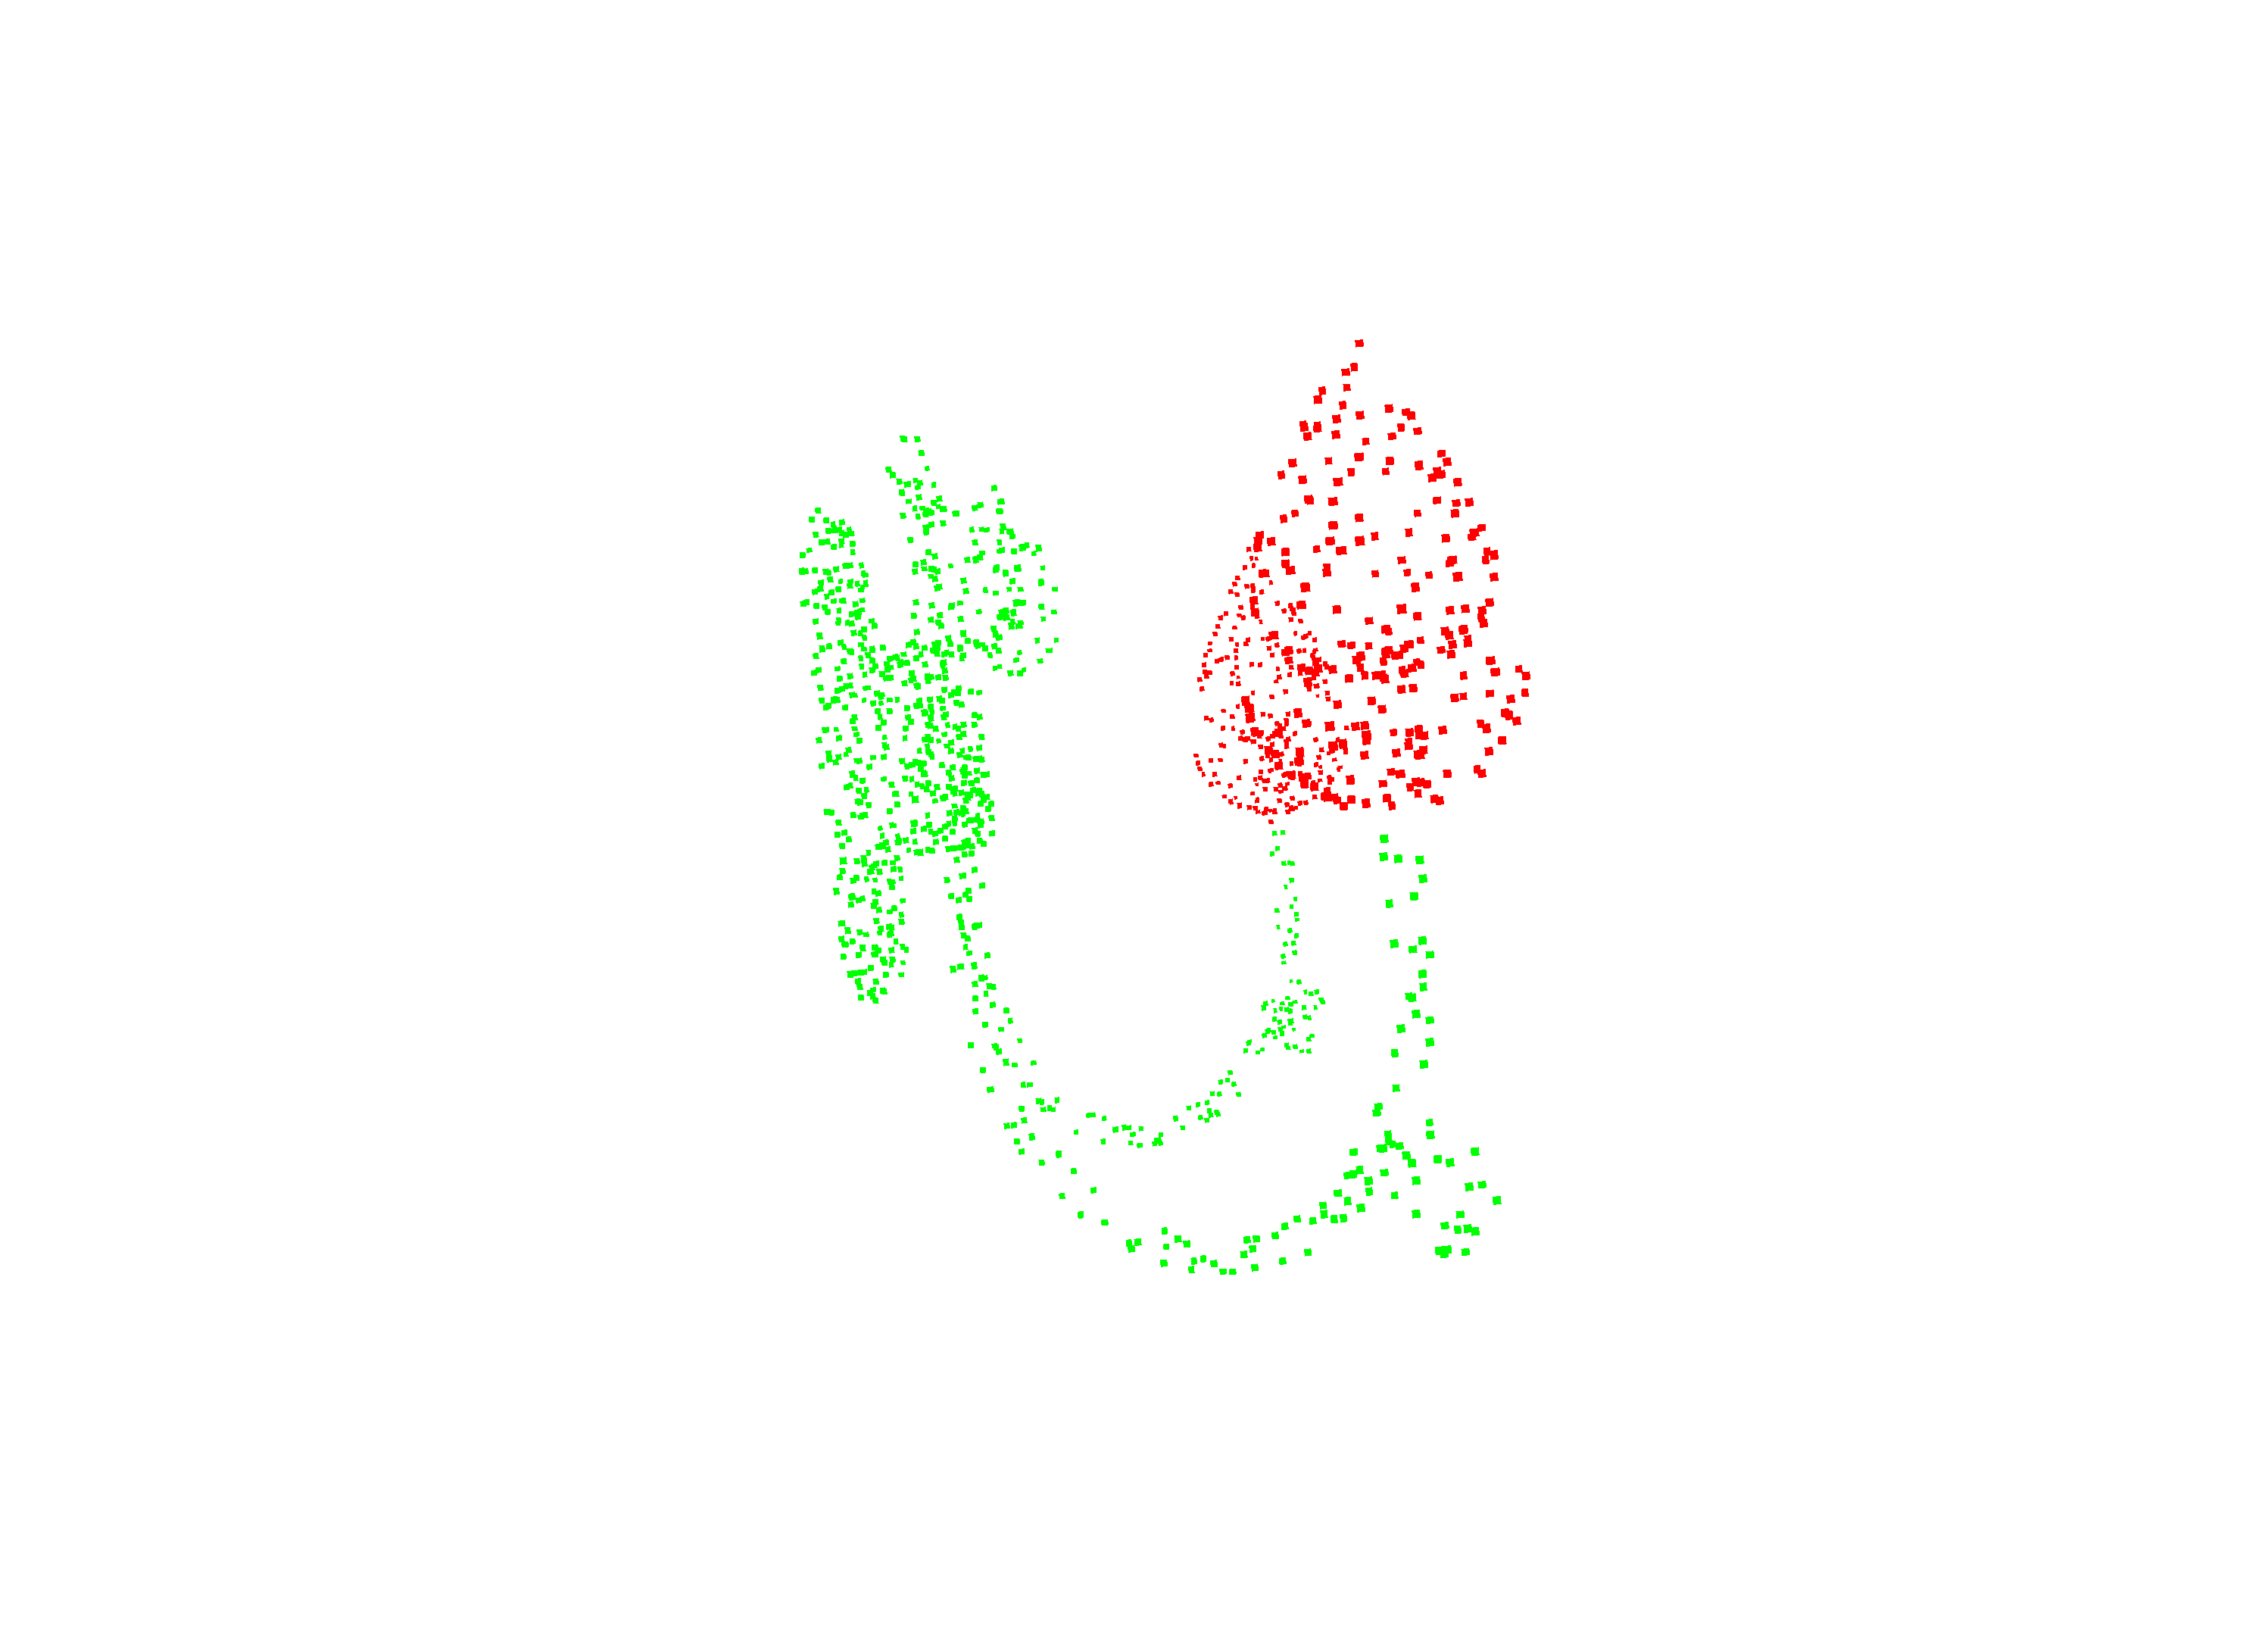
\includegraphics[width=\textwidth]{fig/supplement/part_segmentation/lamp/lamp00.pdf}
    \end{minipage}
    \hfill
    \begin{minipage}{0.25\textwidth}
        \centering
        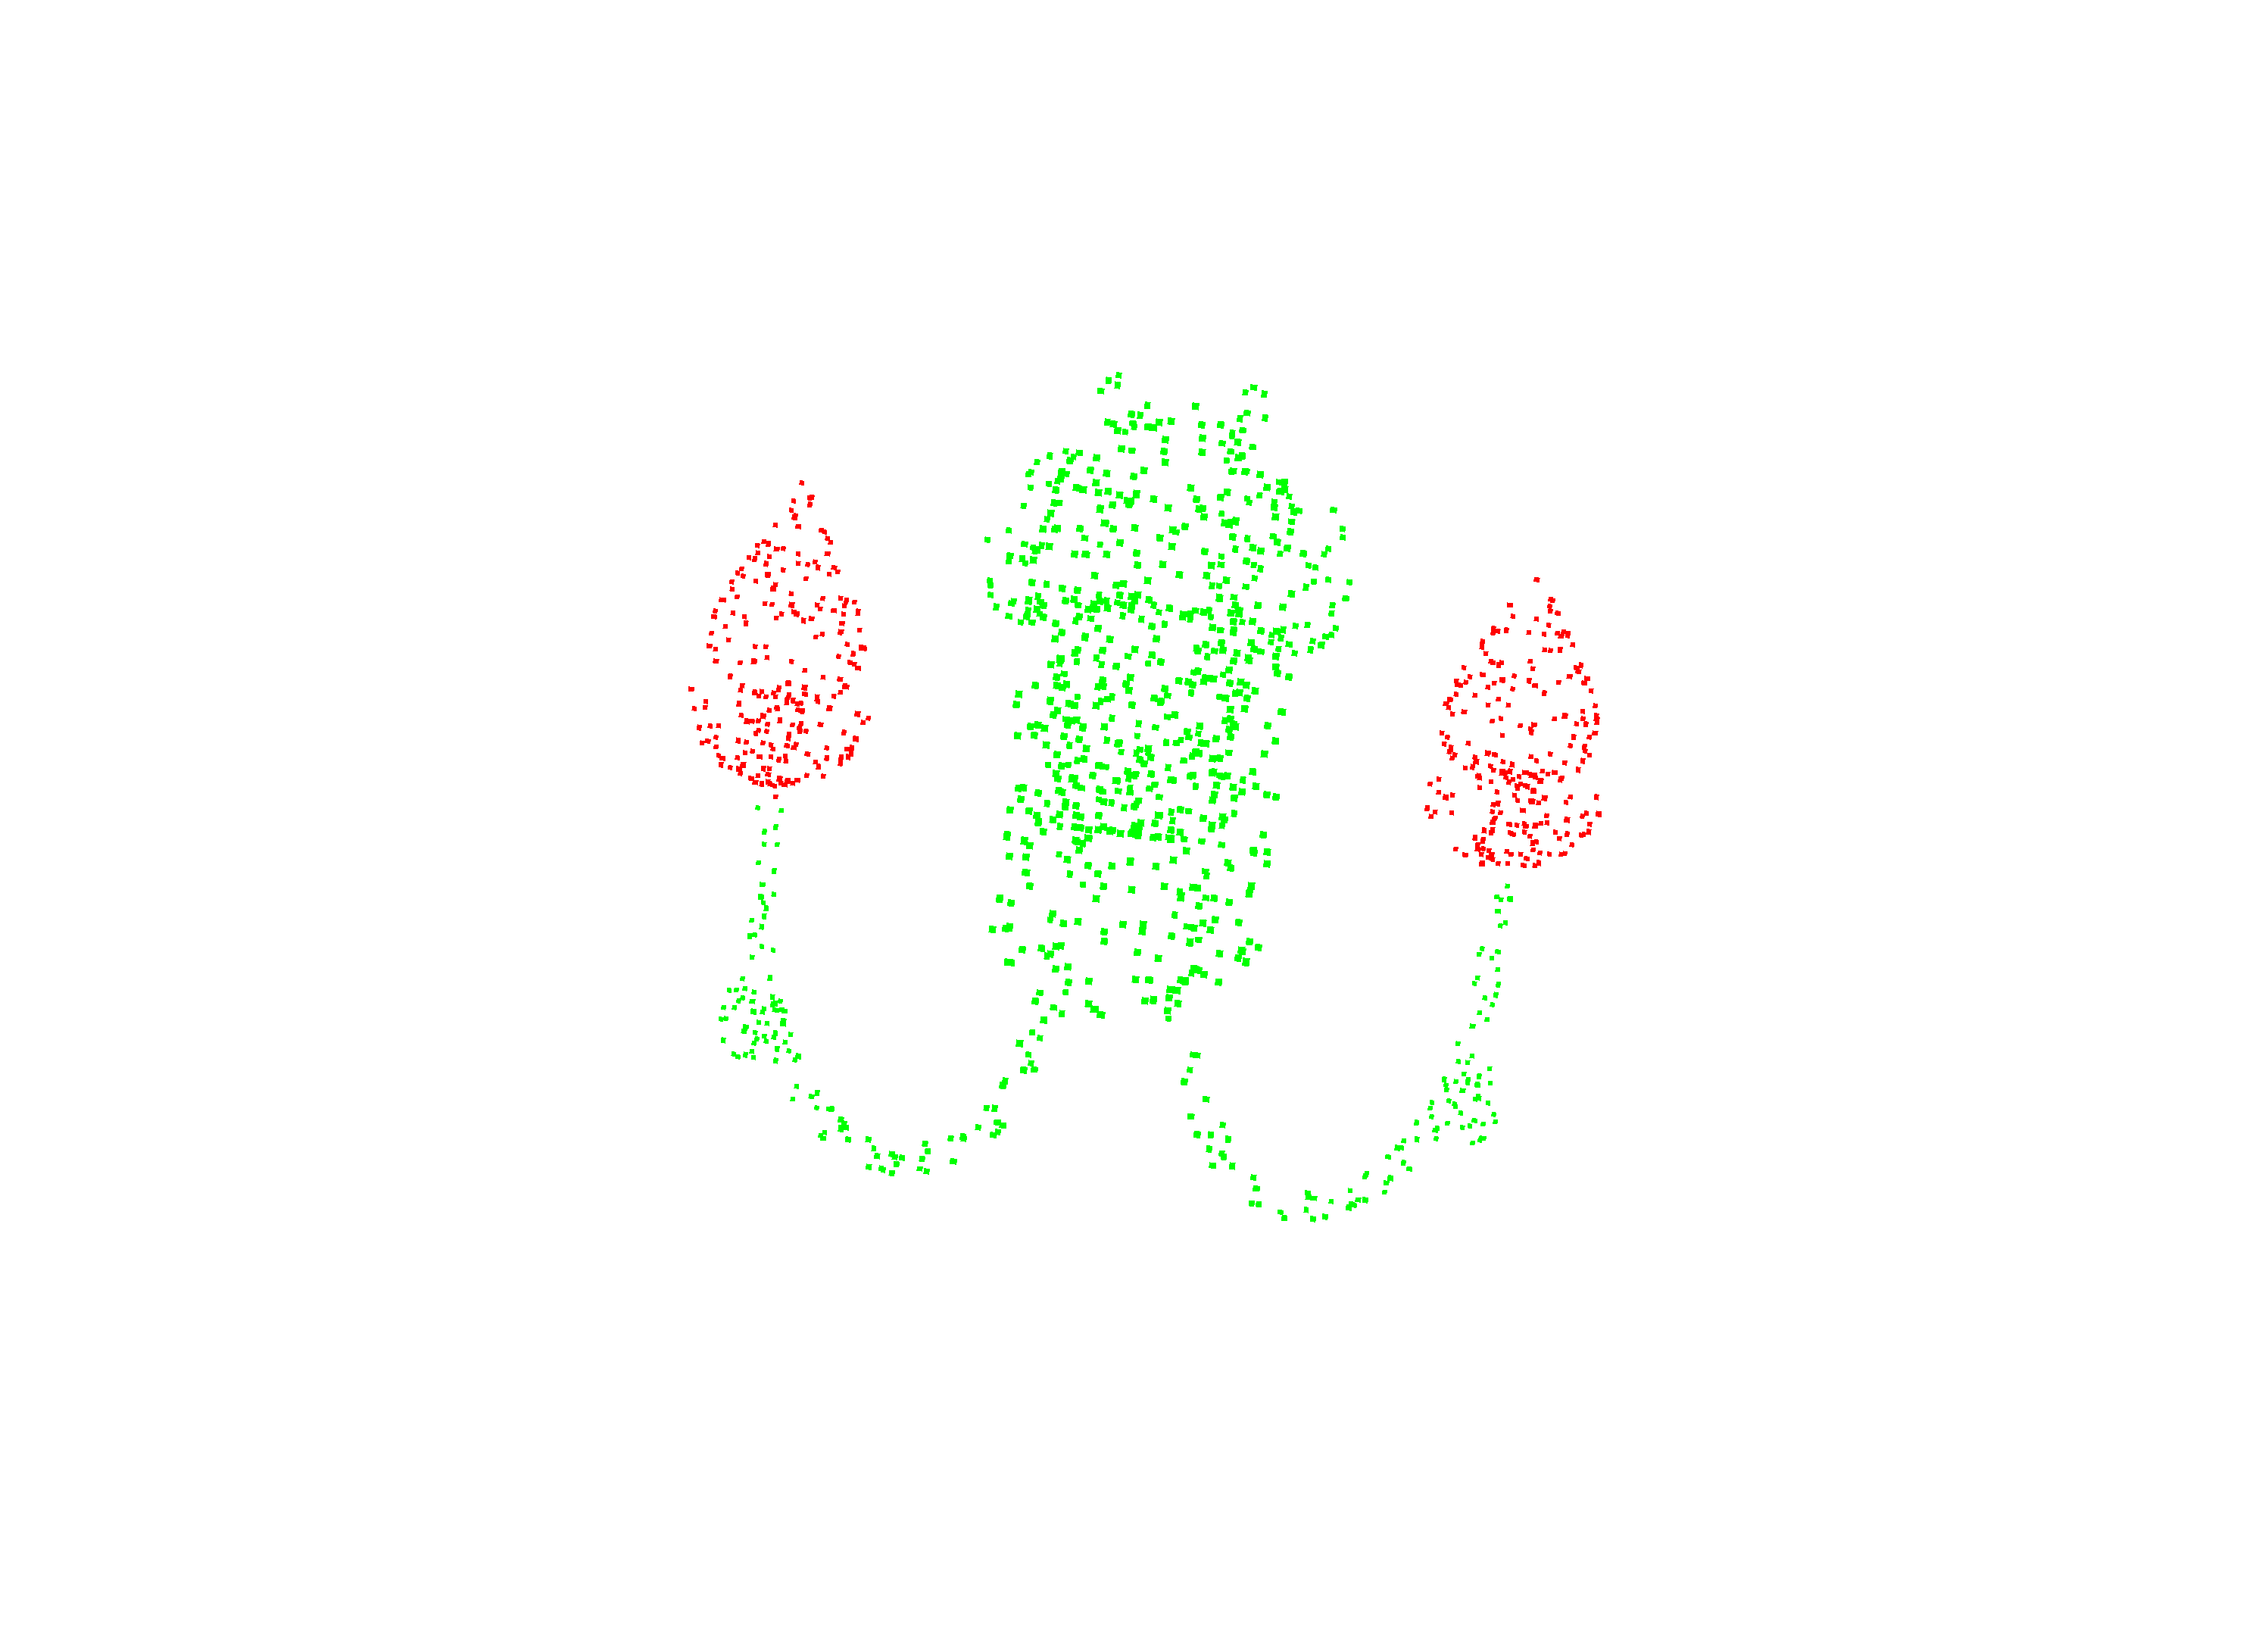
\includegraphics[width=\textwidth]{fig/supplement/part_segmentation/lamp/lamp01.pdf}
    \end{minipage}
    \hfill
    \begin{minipage}{0.25\textwidth}
        \centering
        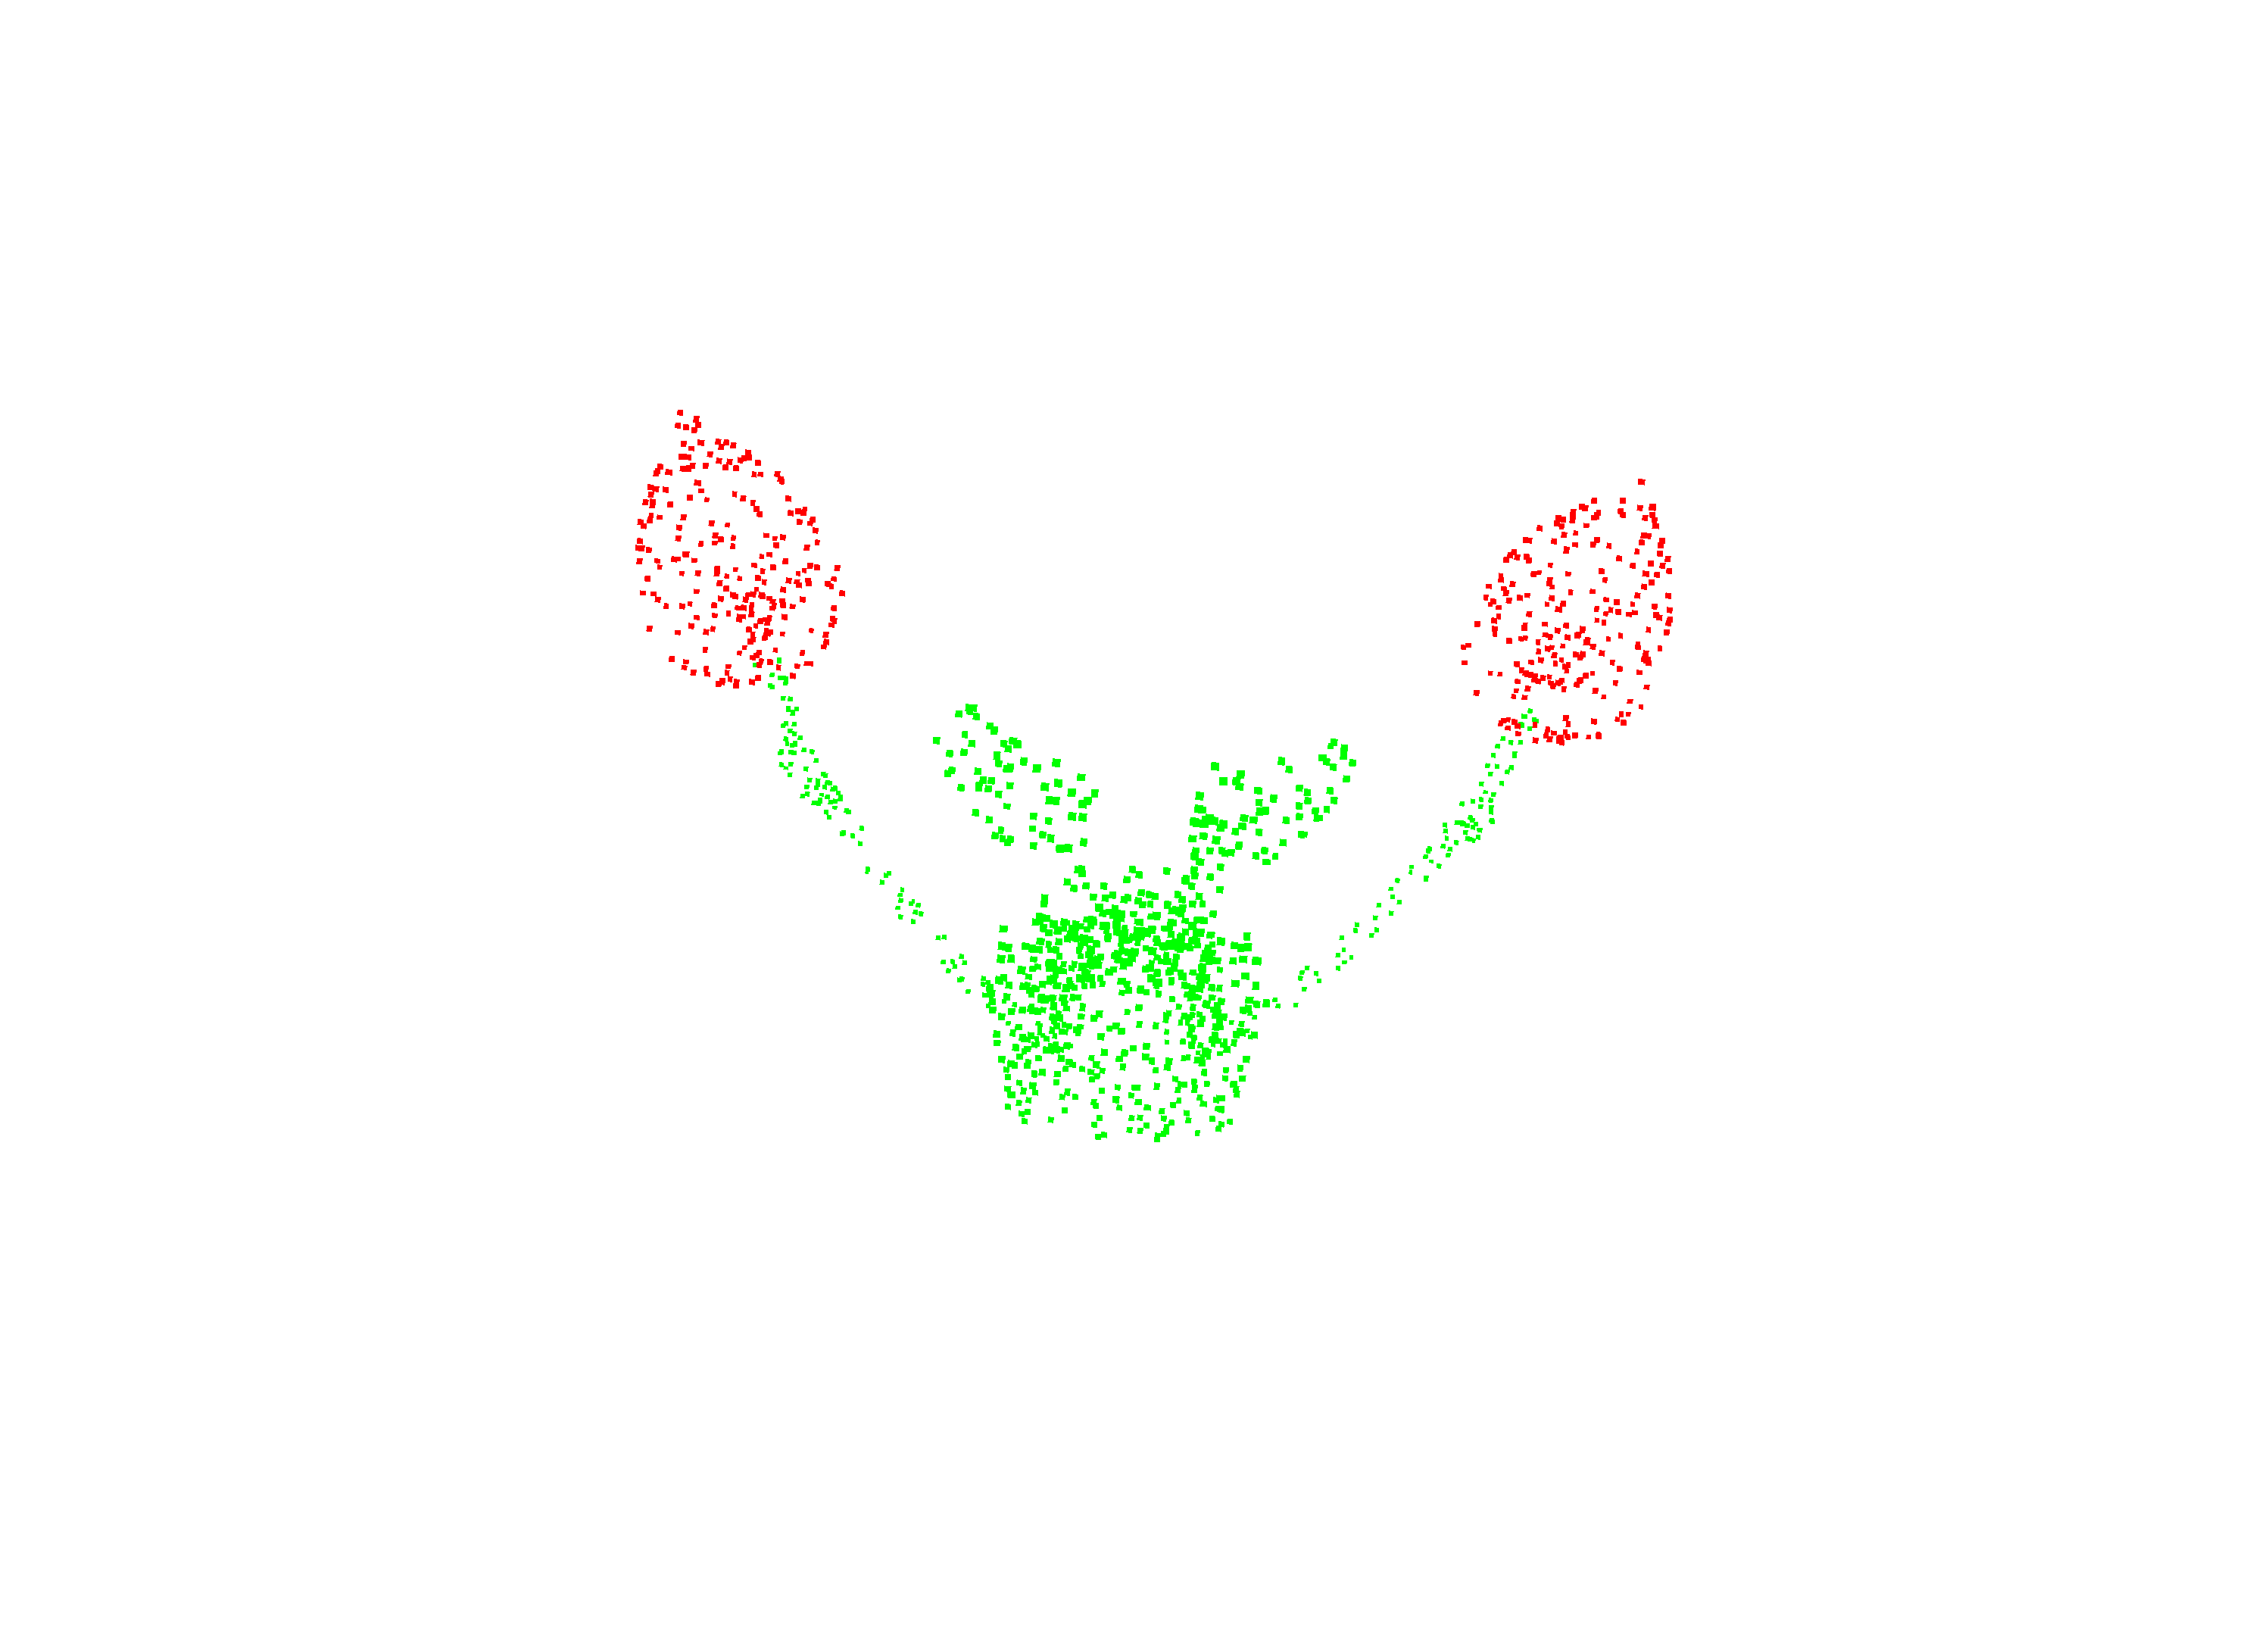
\includegraphics[width=\textwidth]{fig/supplement/part_segmentation/lamp/lamp02.pdf}
    \end{minipage}
    \hfill

    % 换行
    \vspace{0.5em}

    % 第四行左侧的竖排标签
    \begin{minipage}{0.1\textwidth}
        \centering
        {skateboard}
    \end{minipage}
    \hfill
    % 第四行图片
    \begin{minipage}{0.25\textwidth}
        \centering
        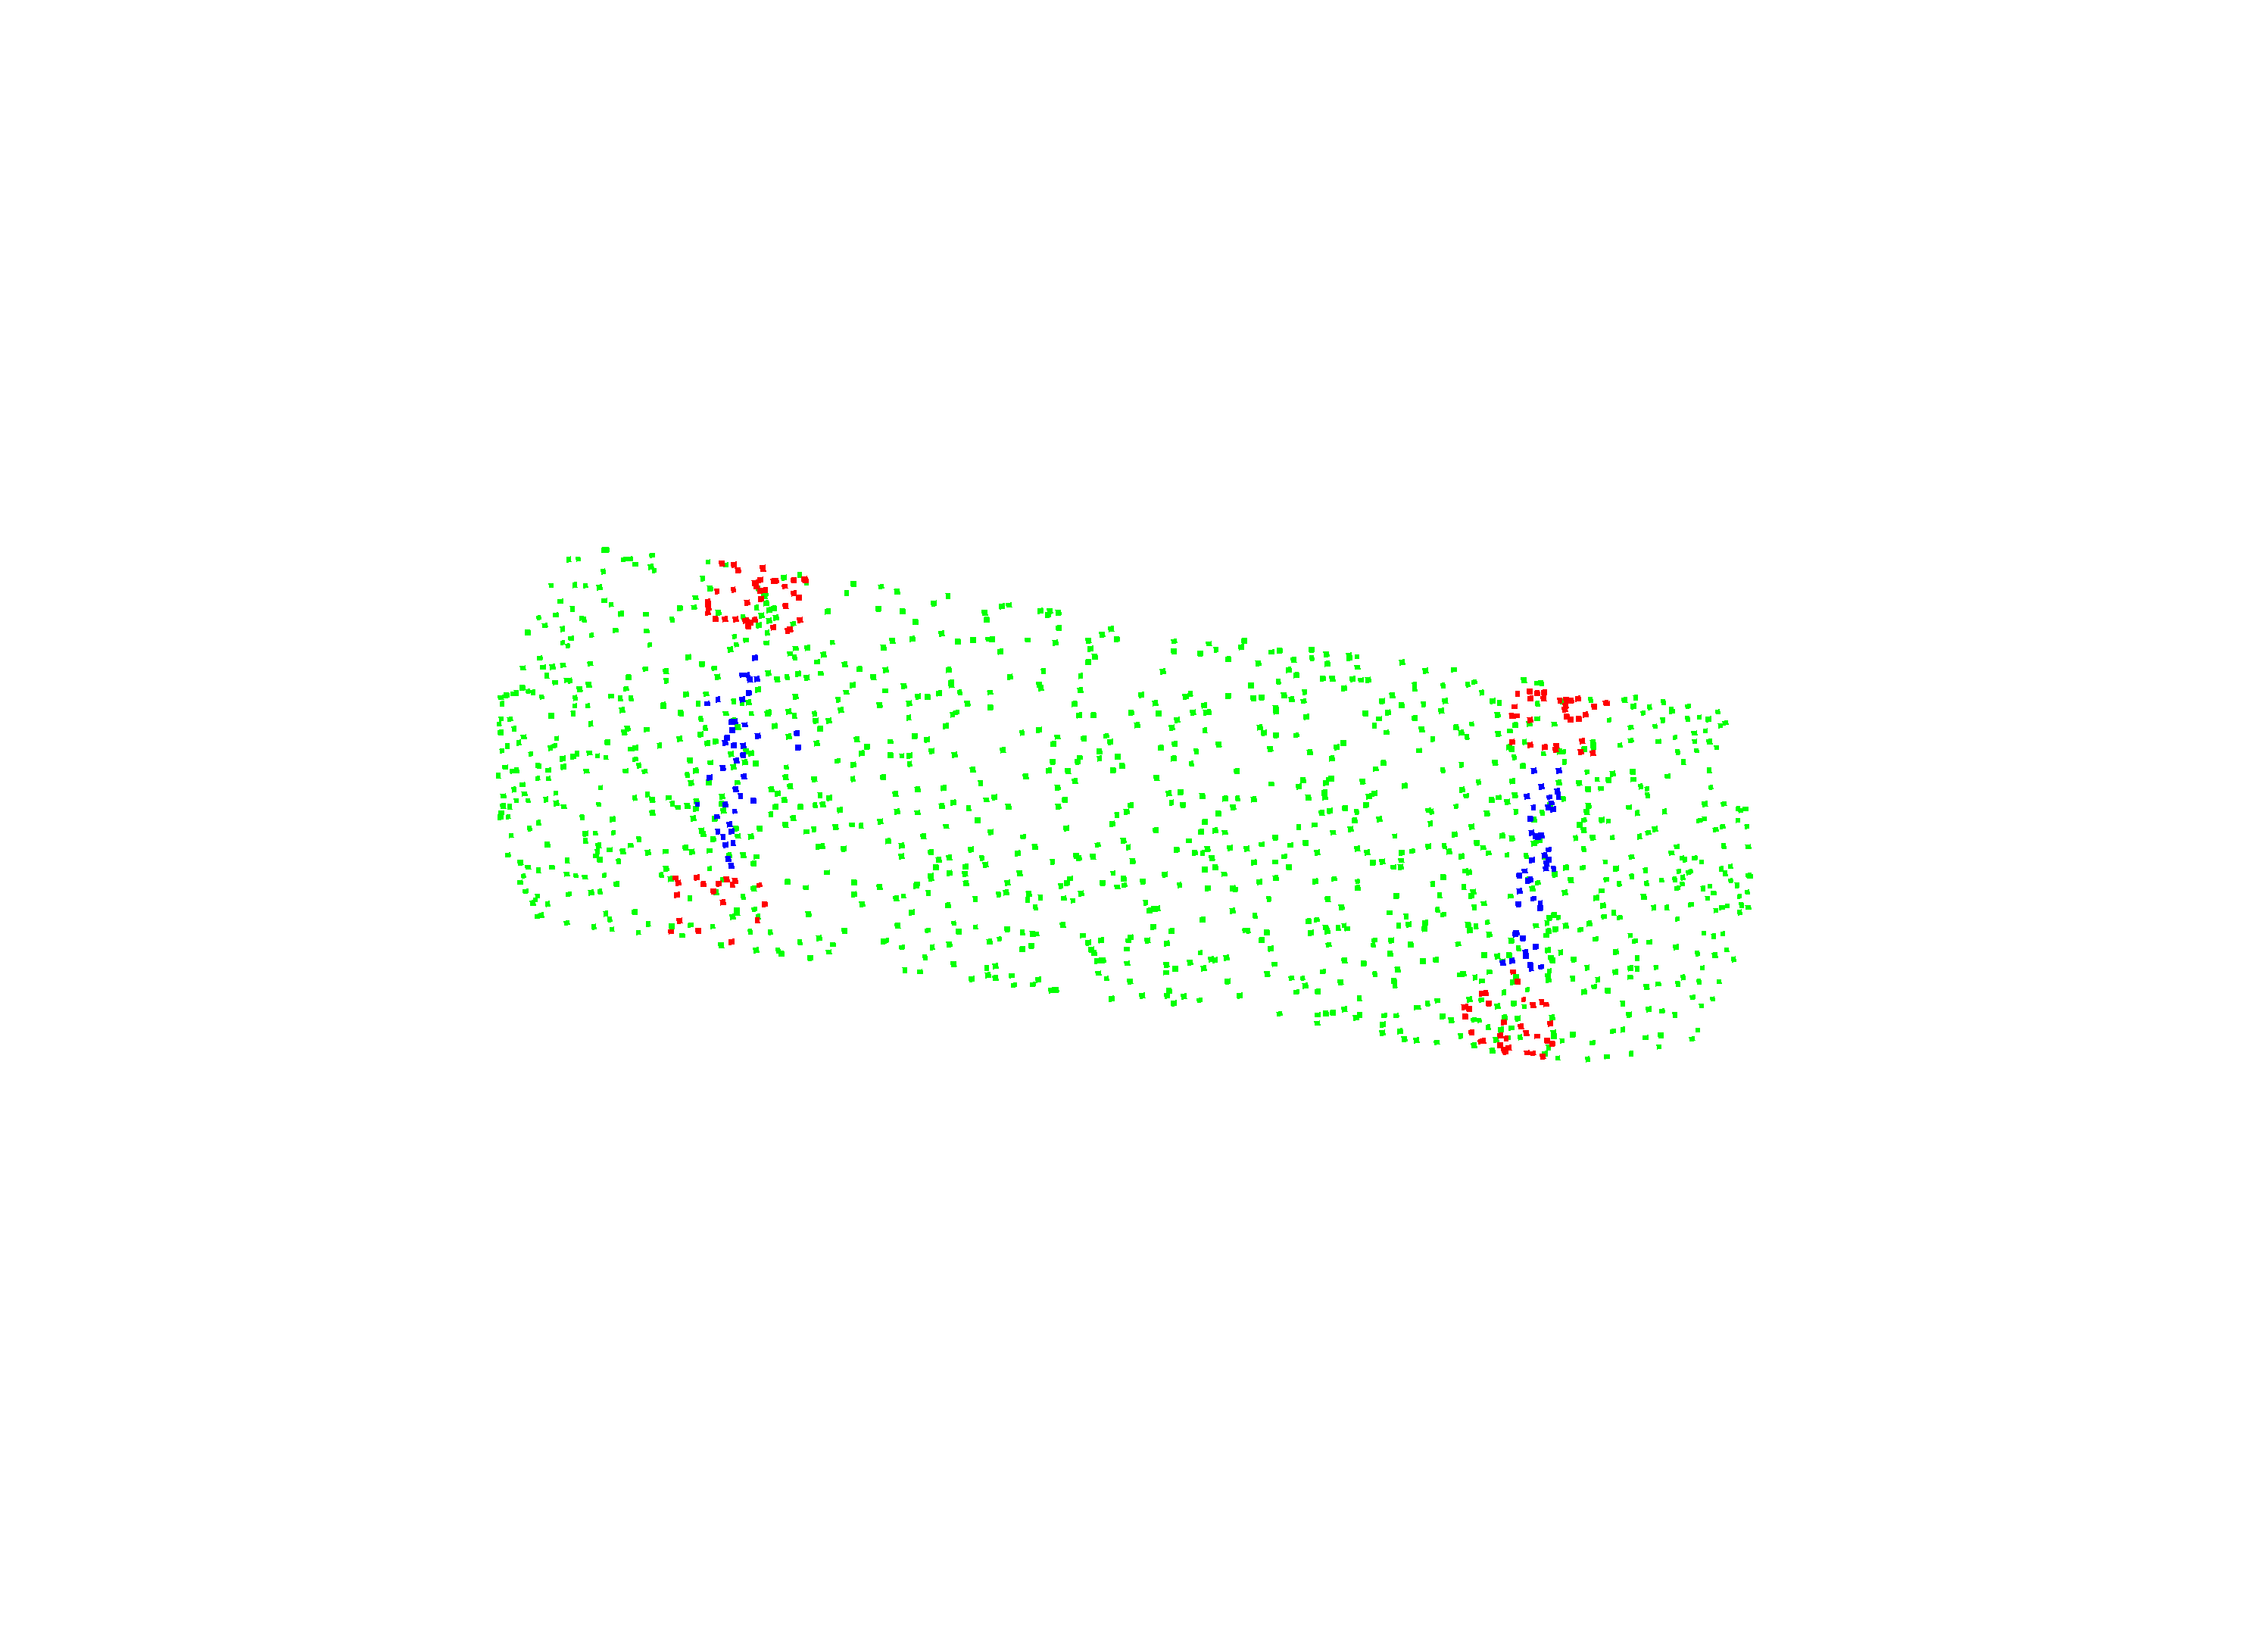
\includegraphics[width=\textwidth]{fig/supplement/part_segmentation/skateboard/skateboard00.pdf}
    \end{minipage}
    \hfill
    \begin{minipage}{0.25\textwidth}
        \centering
        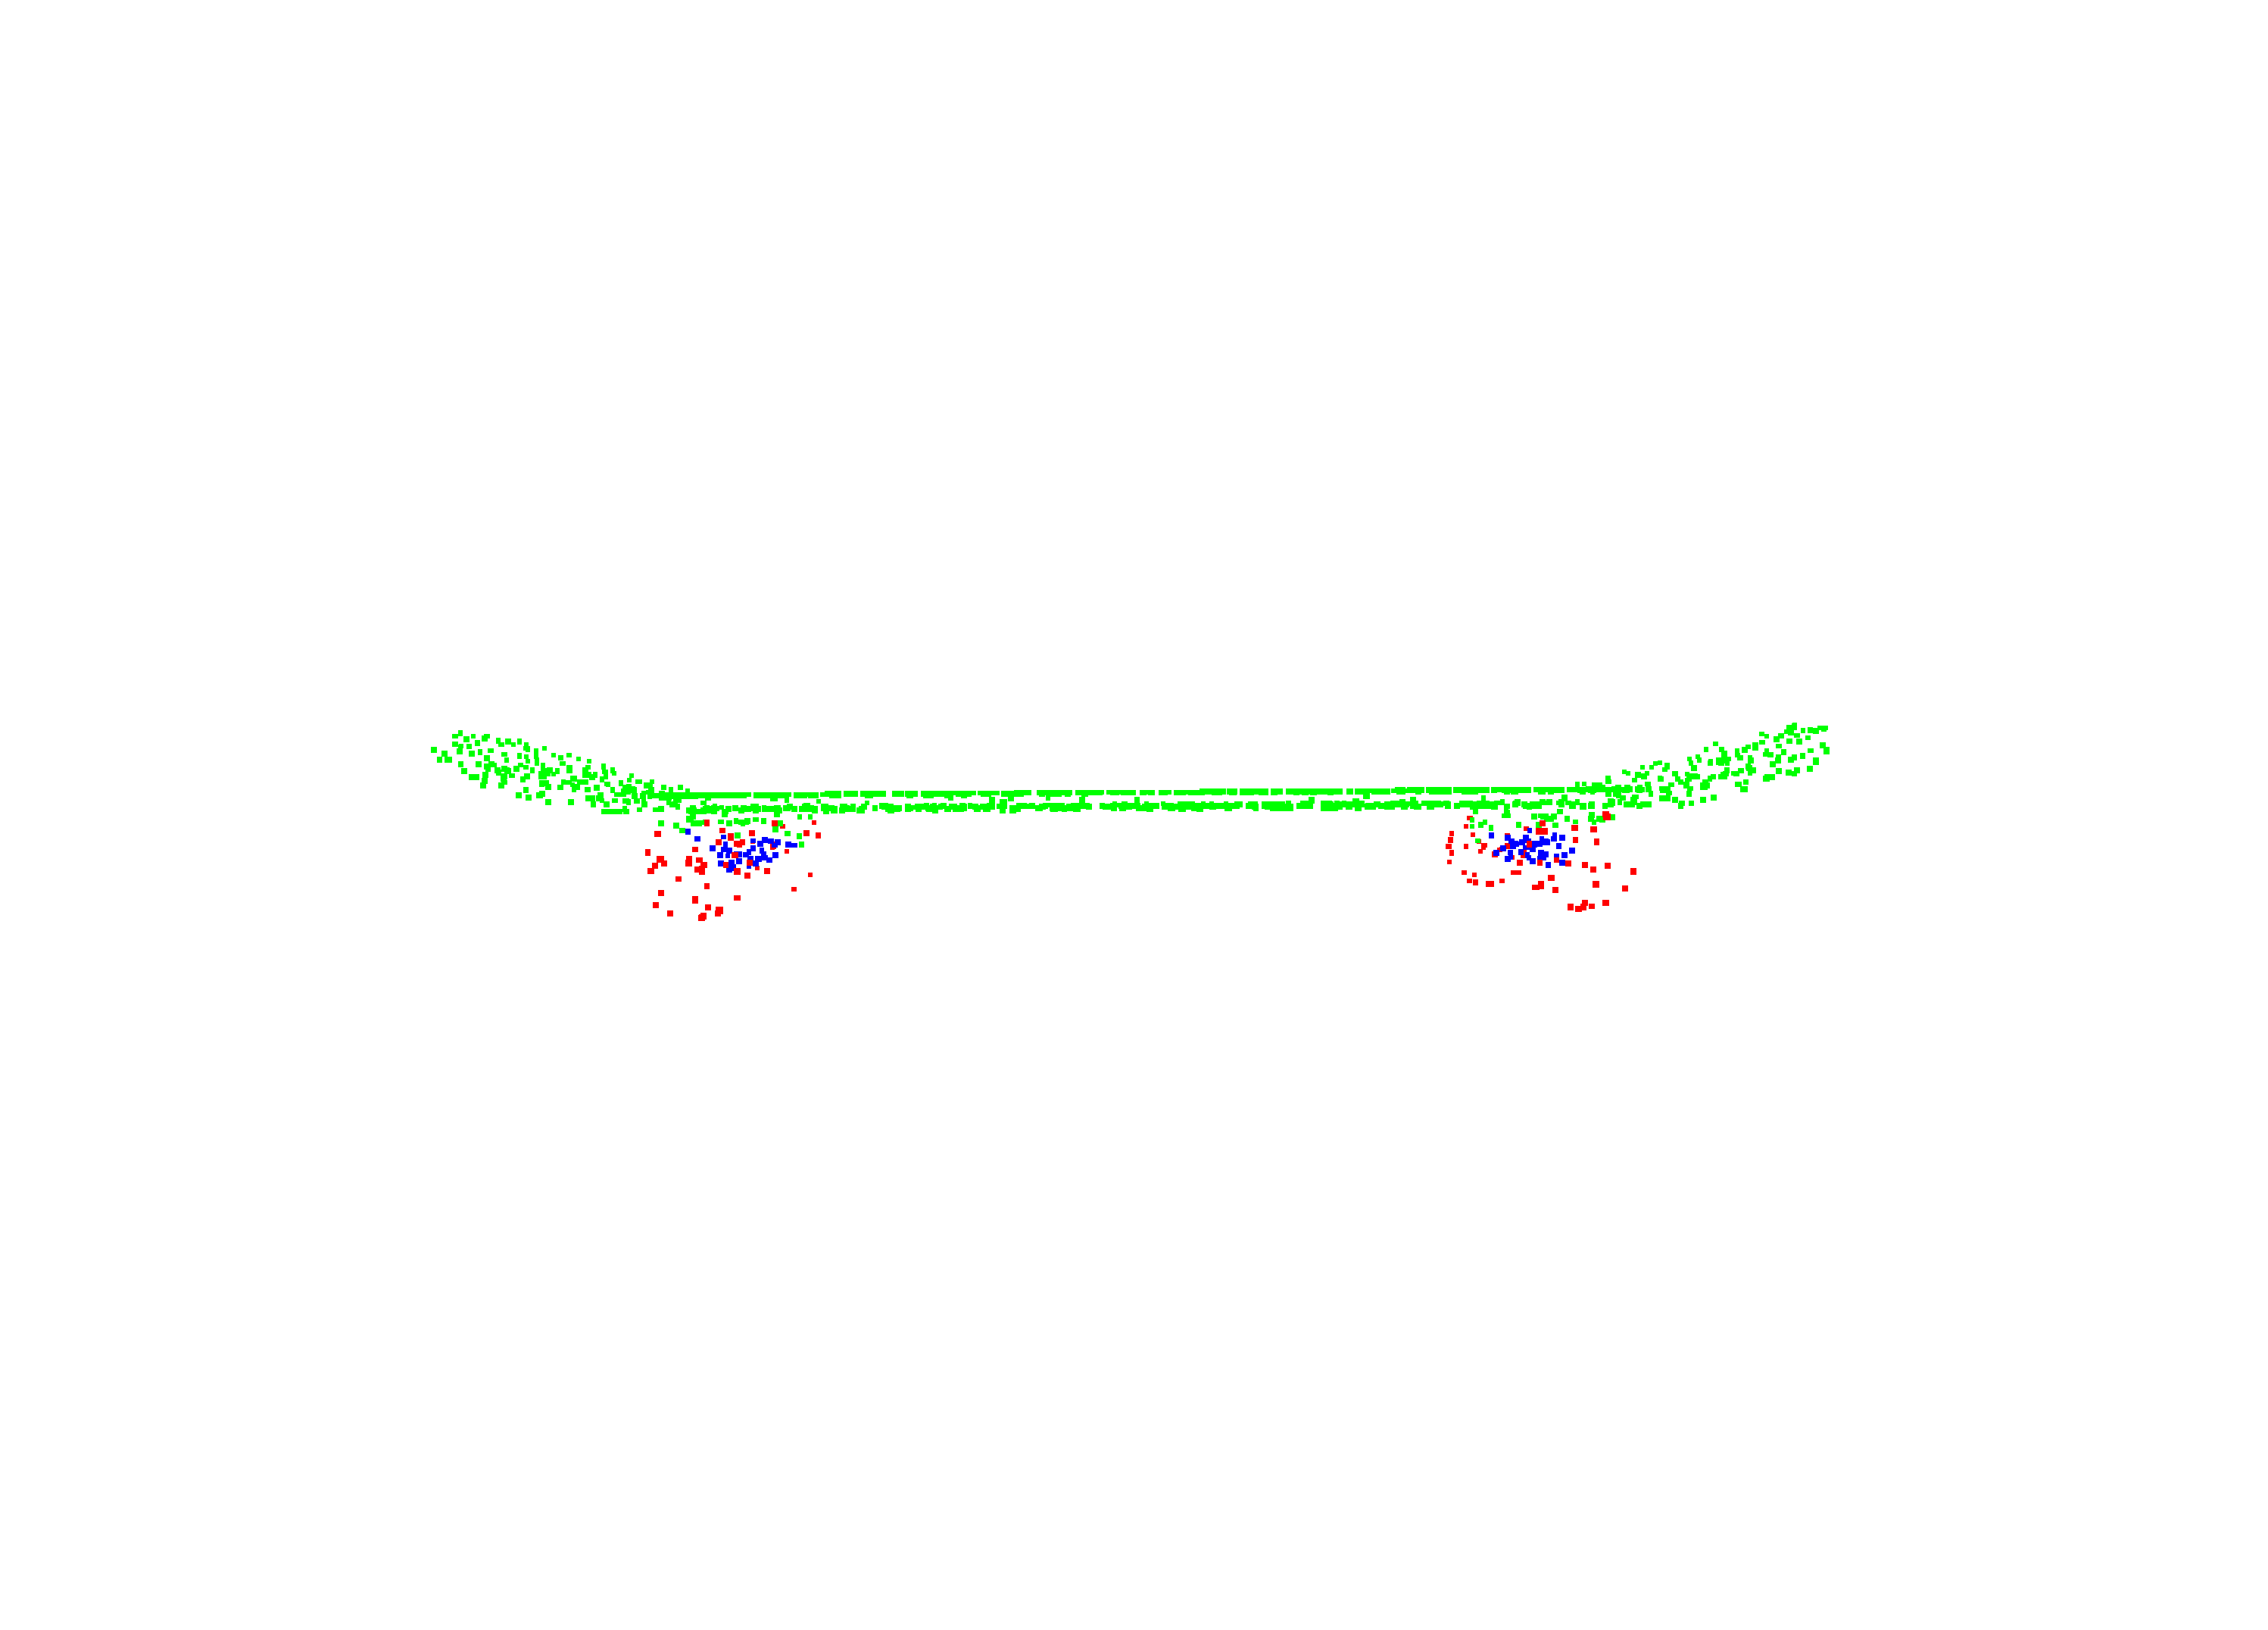
\includegraphics[width=\textwidth]{fig/supplement/part_segmentation/skateboard/skateboard01.pdf}
    \end{minipage}
    \hfill
    \begin{minipage}{0.25\textwidth}
        \centering
        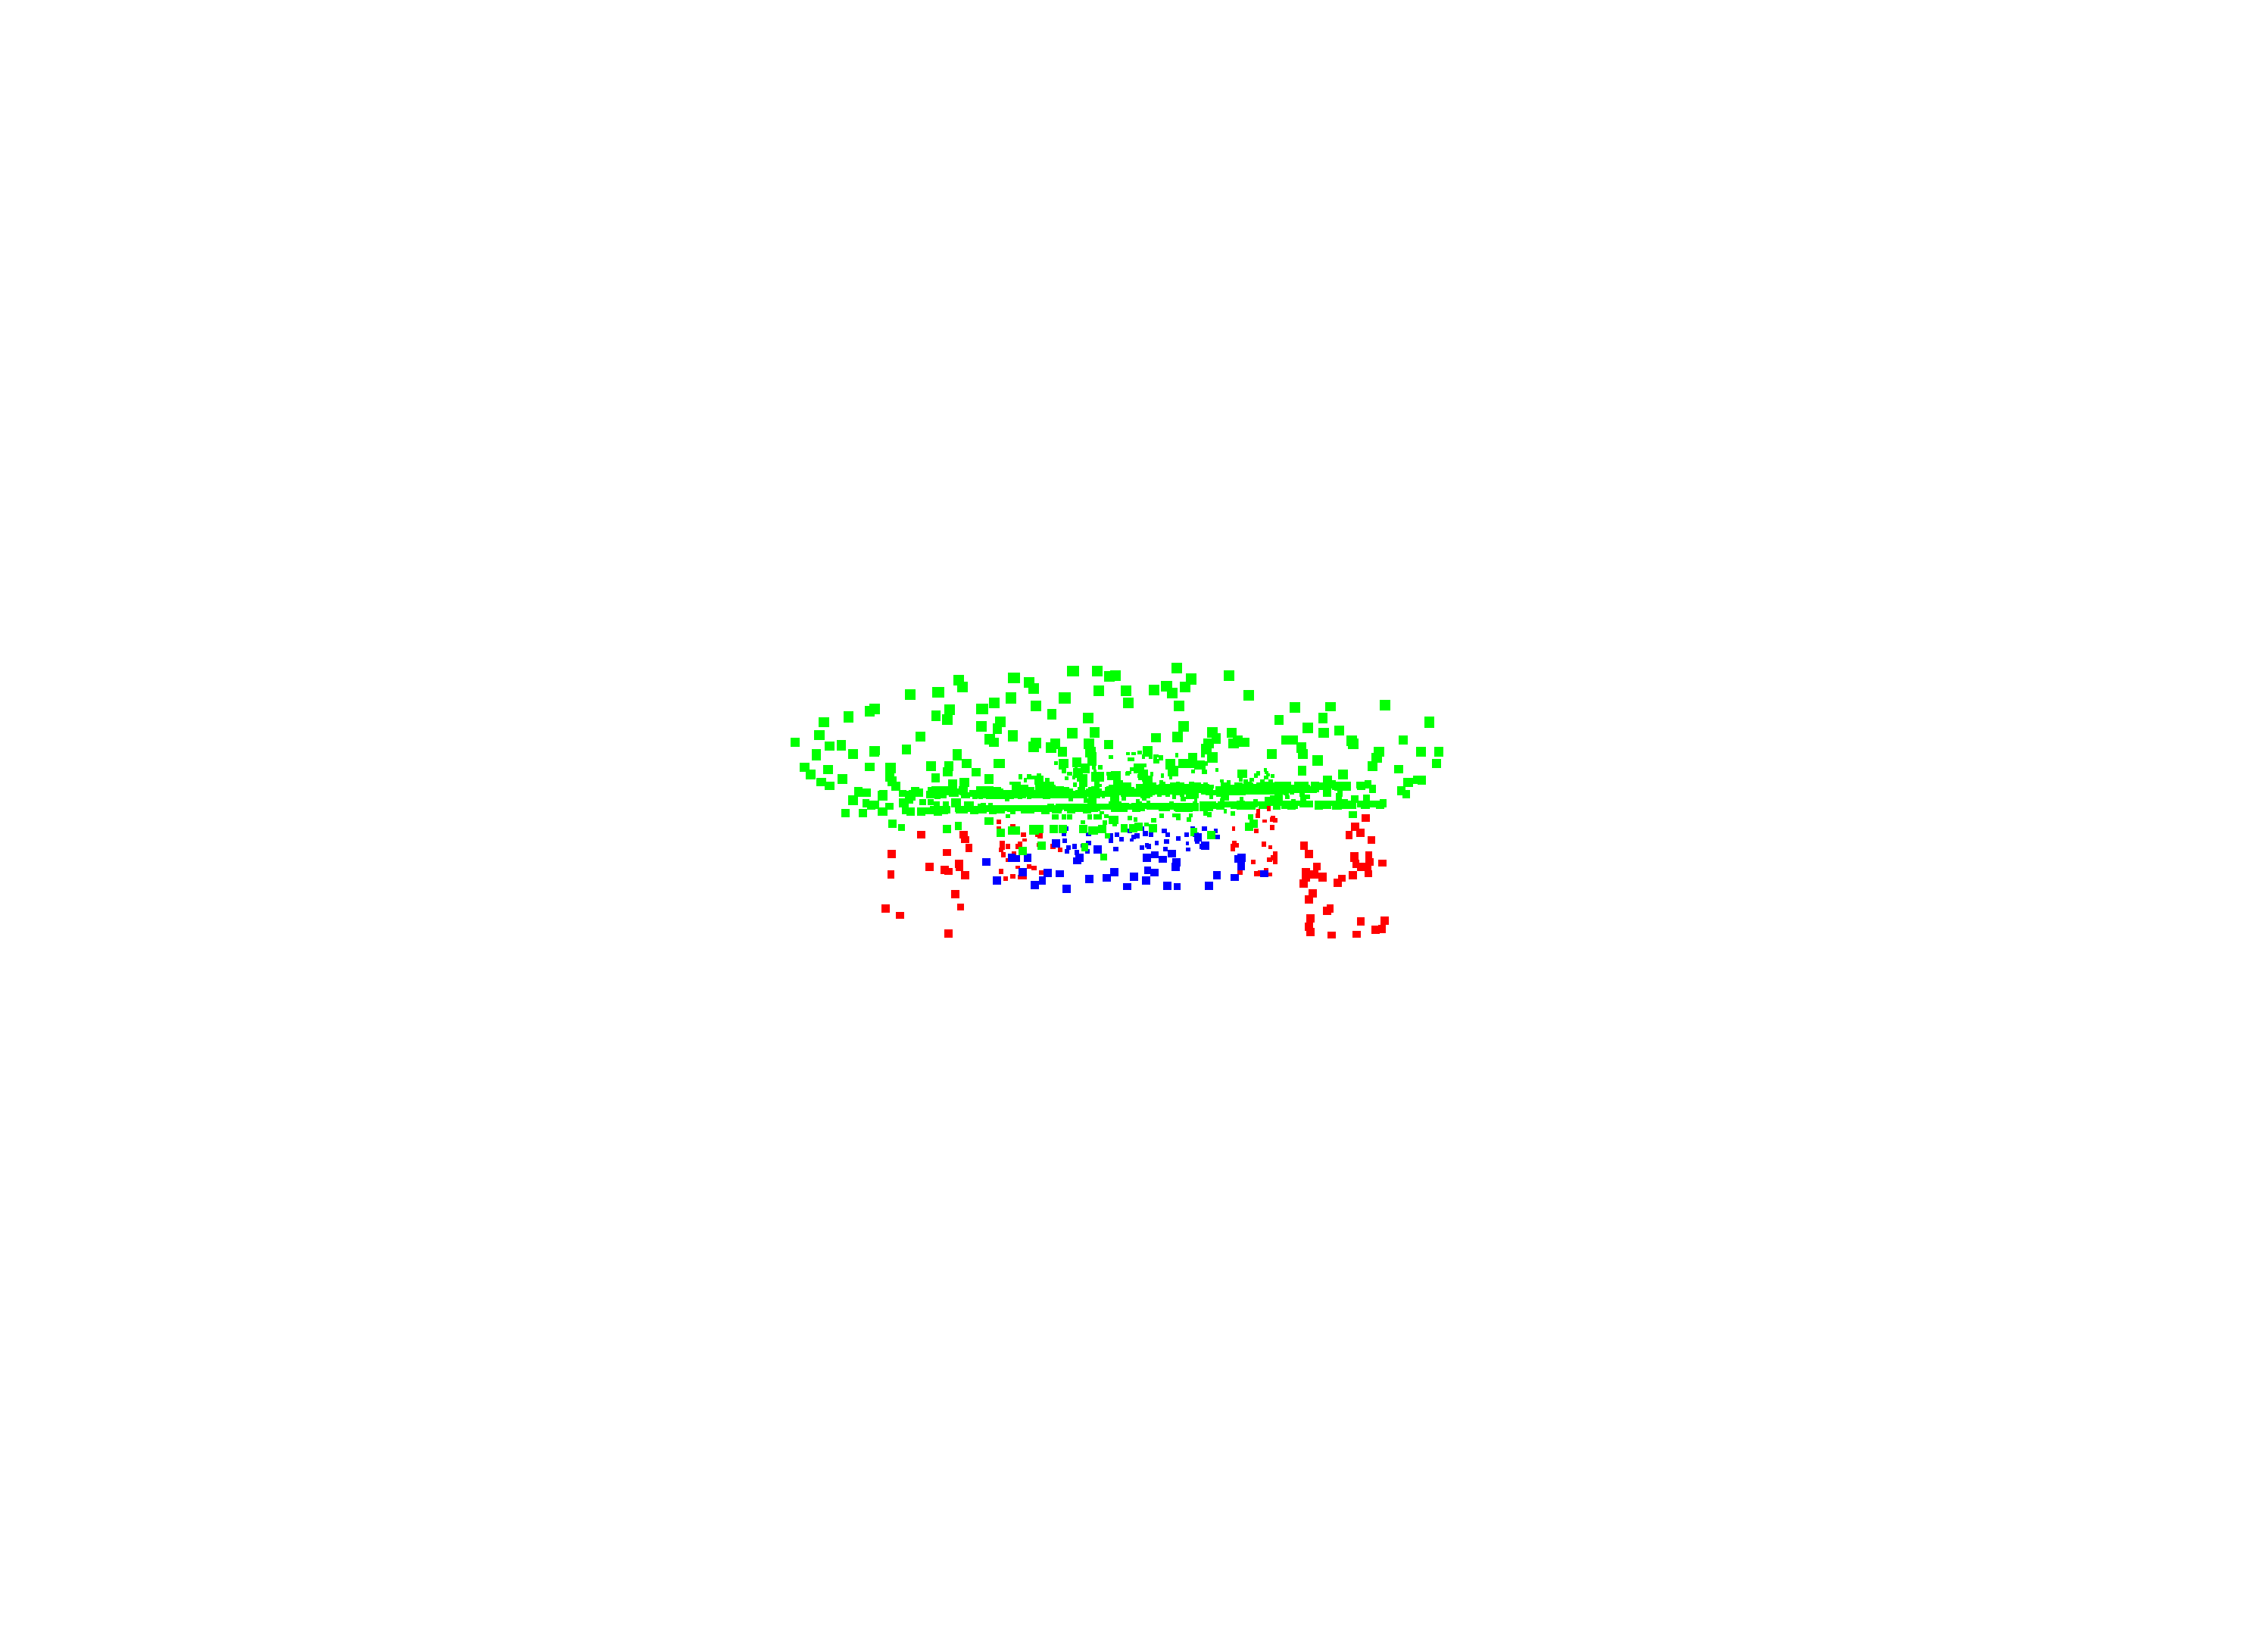
\includegraphics[width=\textwidth]{fig/supplement/part_segmentation/skateboard/skateboard02.pdf}
    \end{minipage}
    \hfill

    % 换行
    \vspace{0.5em}

    % 第五行左侧的竖排标签
    \begin{minipage}{0.1\textwidth}
        \centering
        {table}
    \end{minipage}
    \hfill
    % 第五行图片
    \begin{minipage}{0.25\textwidth}
        \centering
        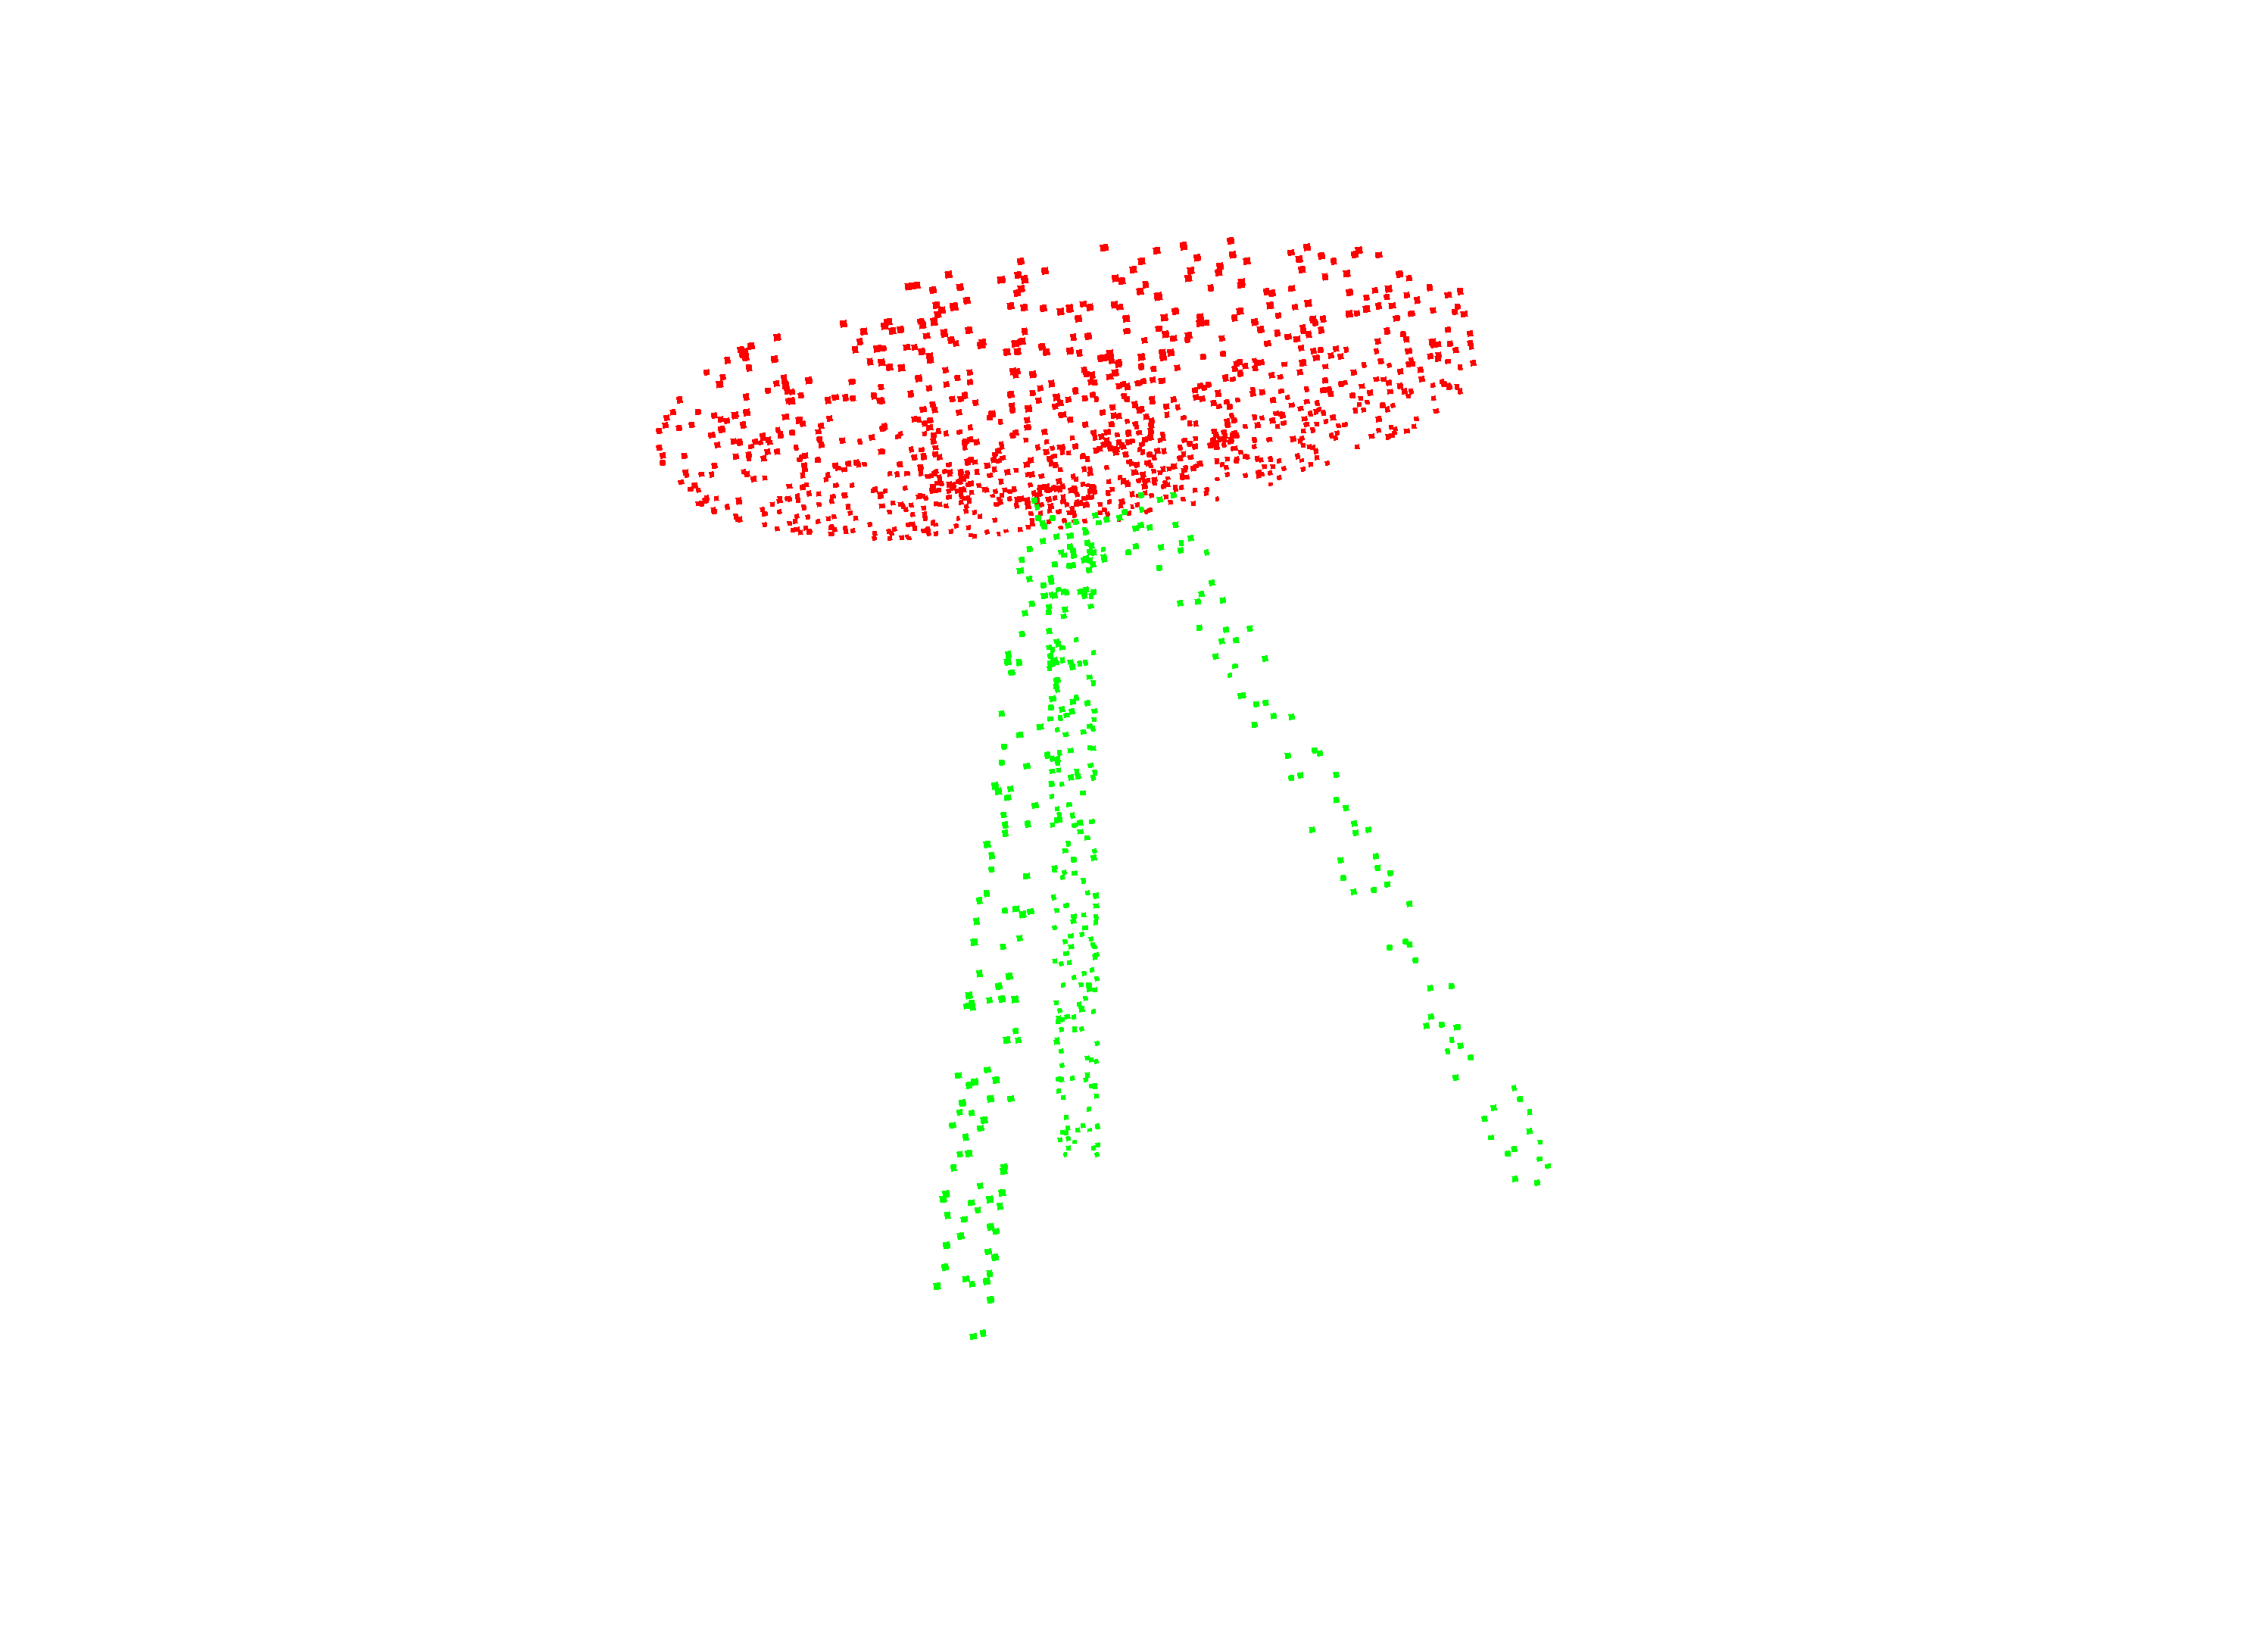
\includegraphics[width=\textwidth]{fig/supplement/part_segmentation/table/table00.pdf}
    \end{minipage}
    \hfill
    \begin{minipage}{0.25\textwidth}
        \centering
        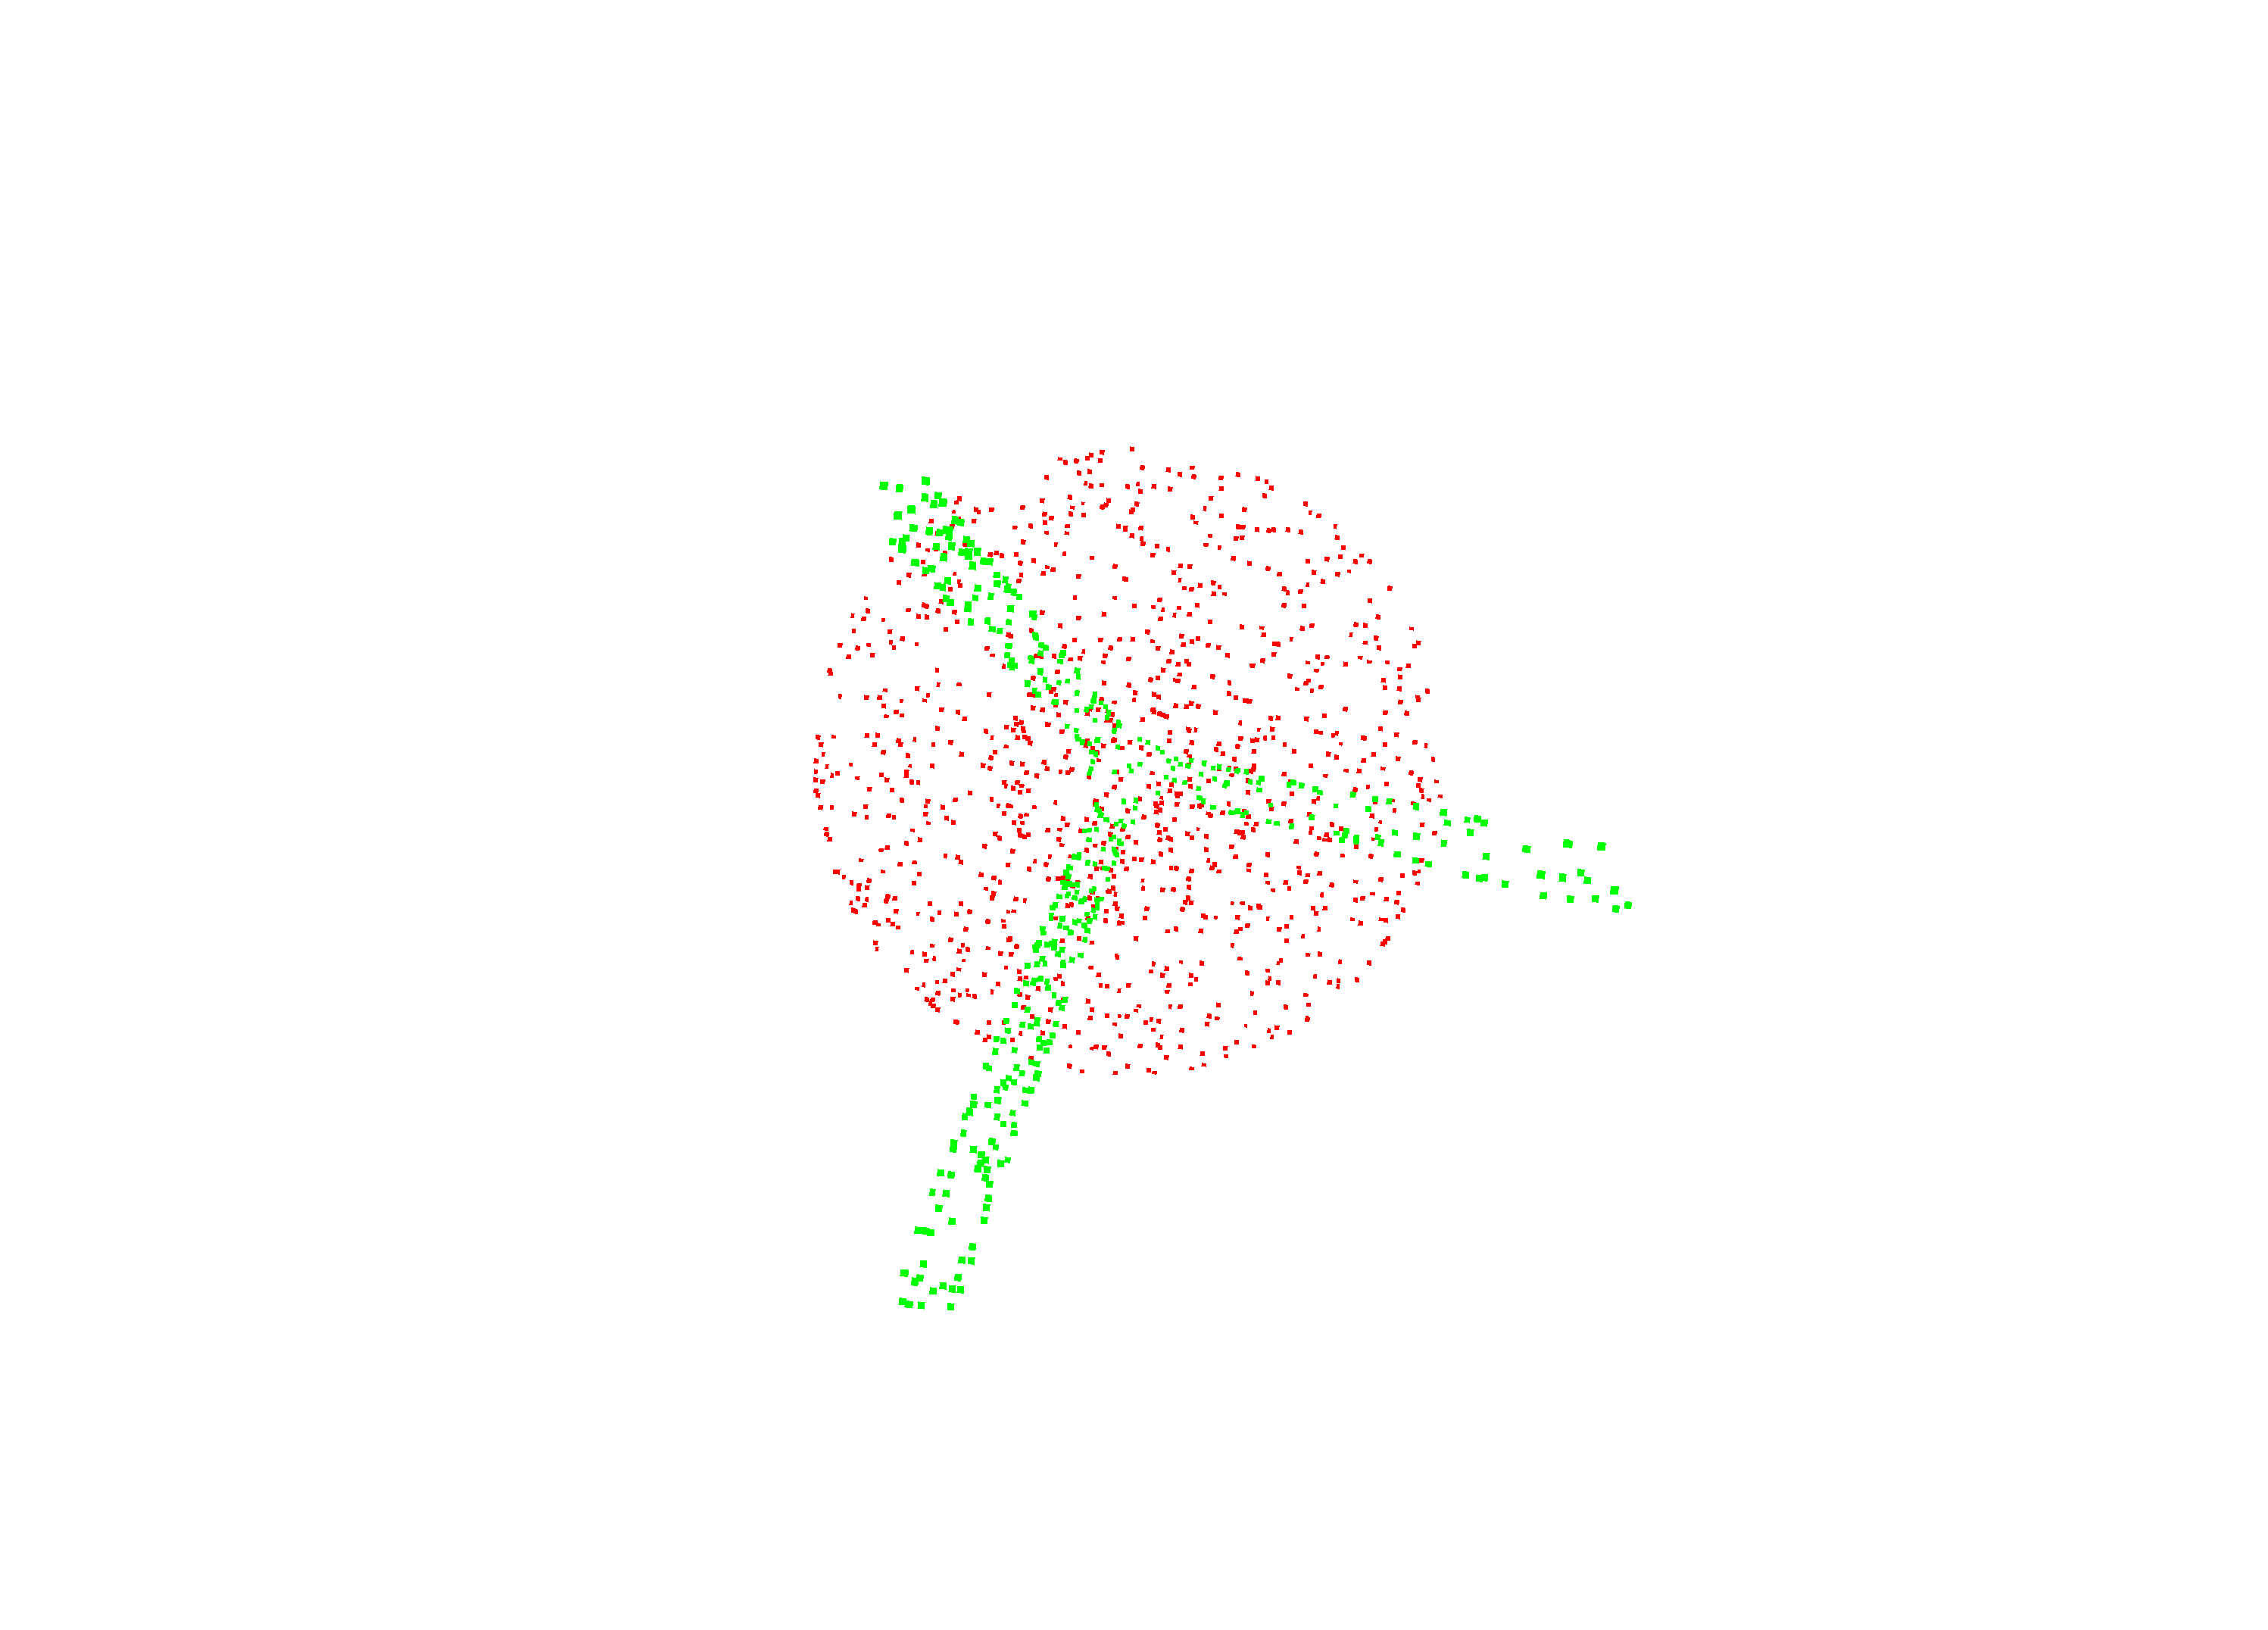
\includegraphics[width=\textwidth]{fig/supplement/part_segmentation/table/table01.pdf}
    \end{minipage}
    \hfill
    \begin{minipage}{0.25\textwidth}
        \centering
        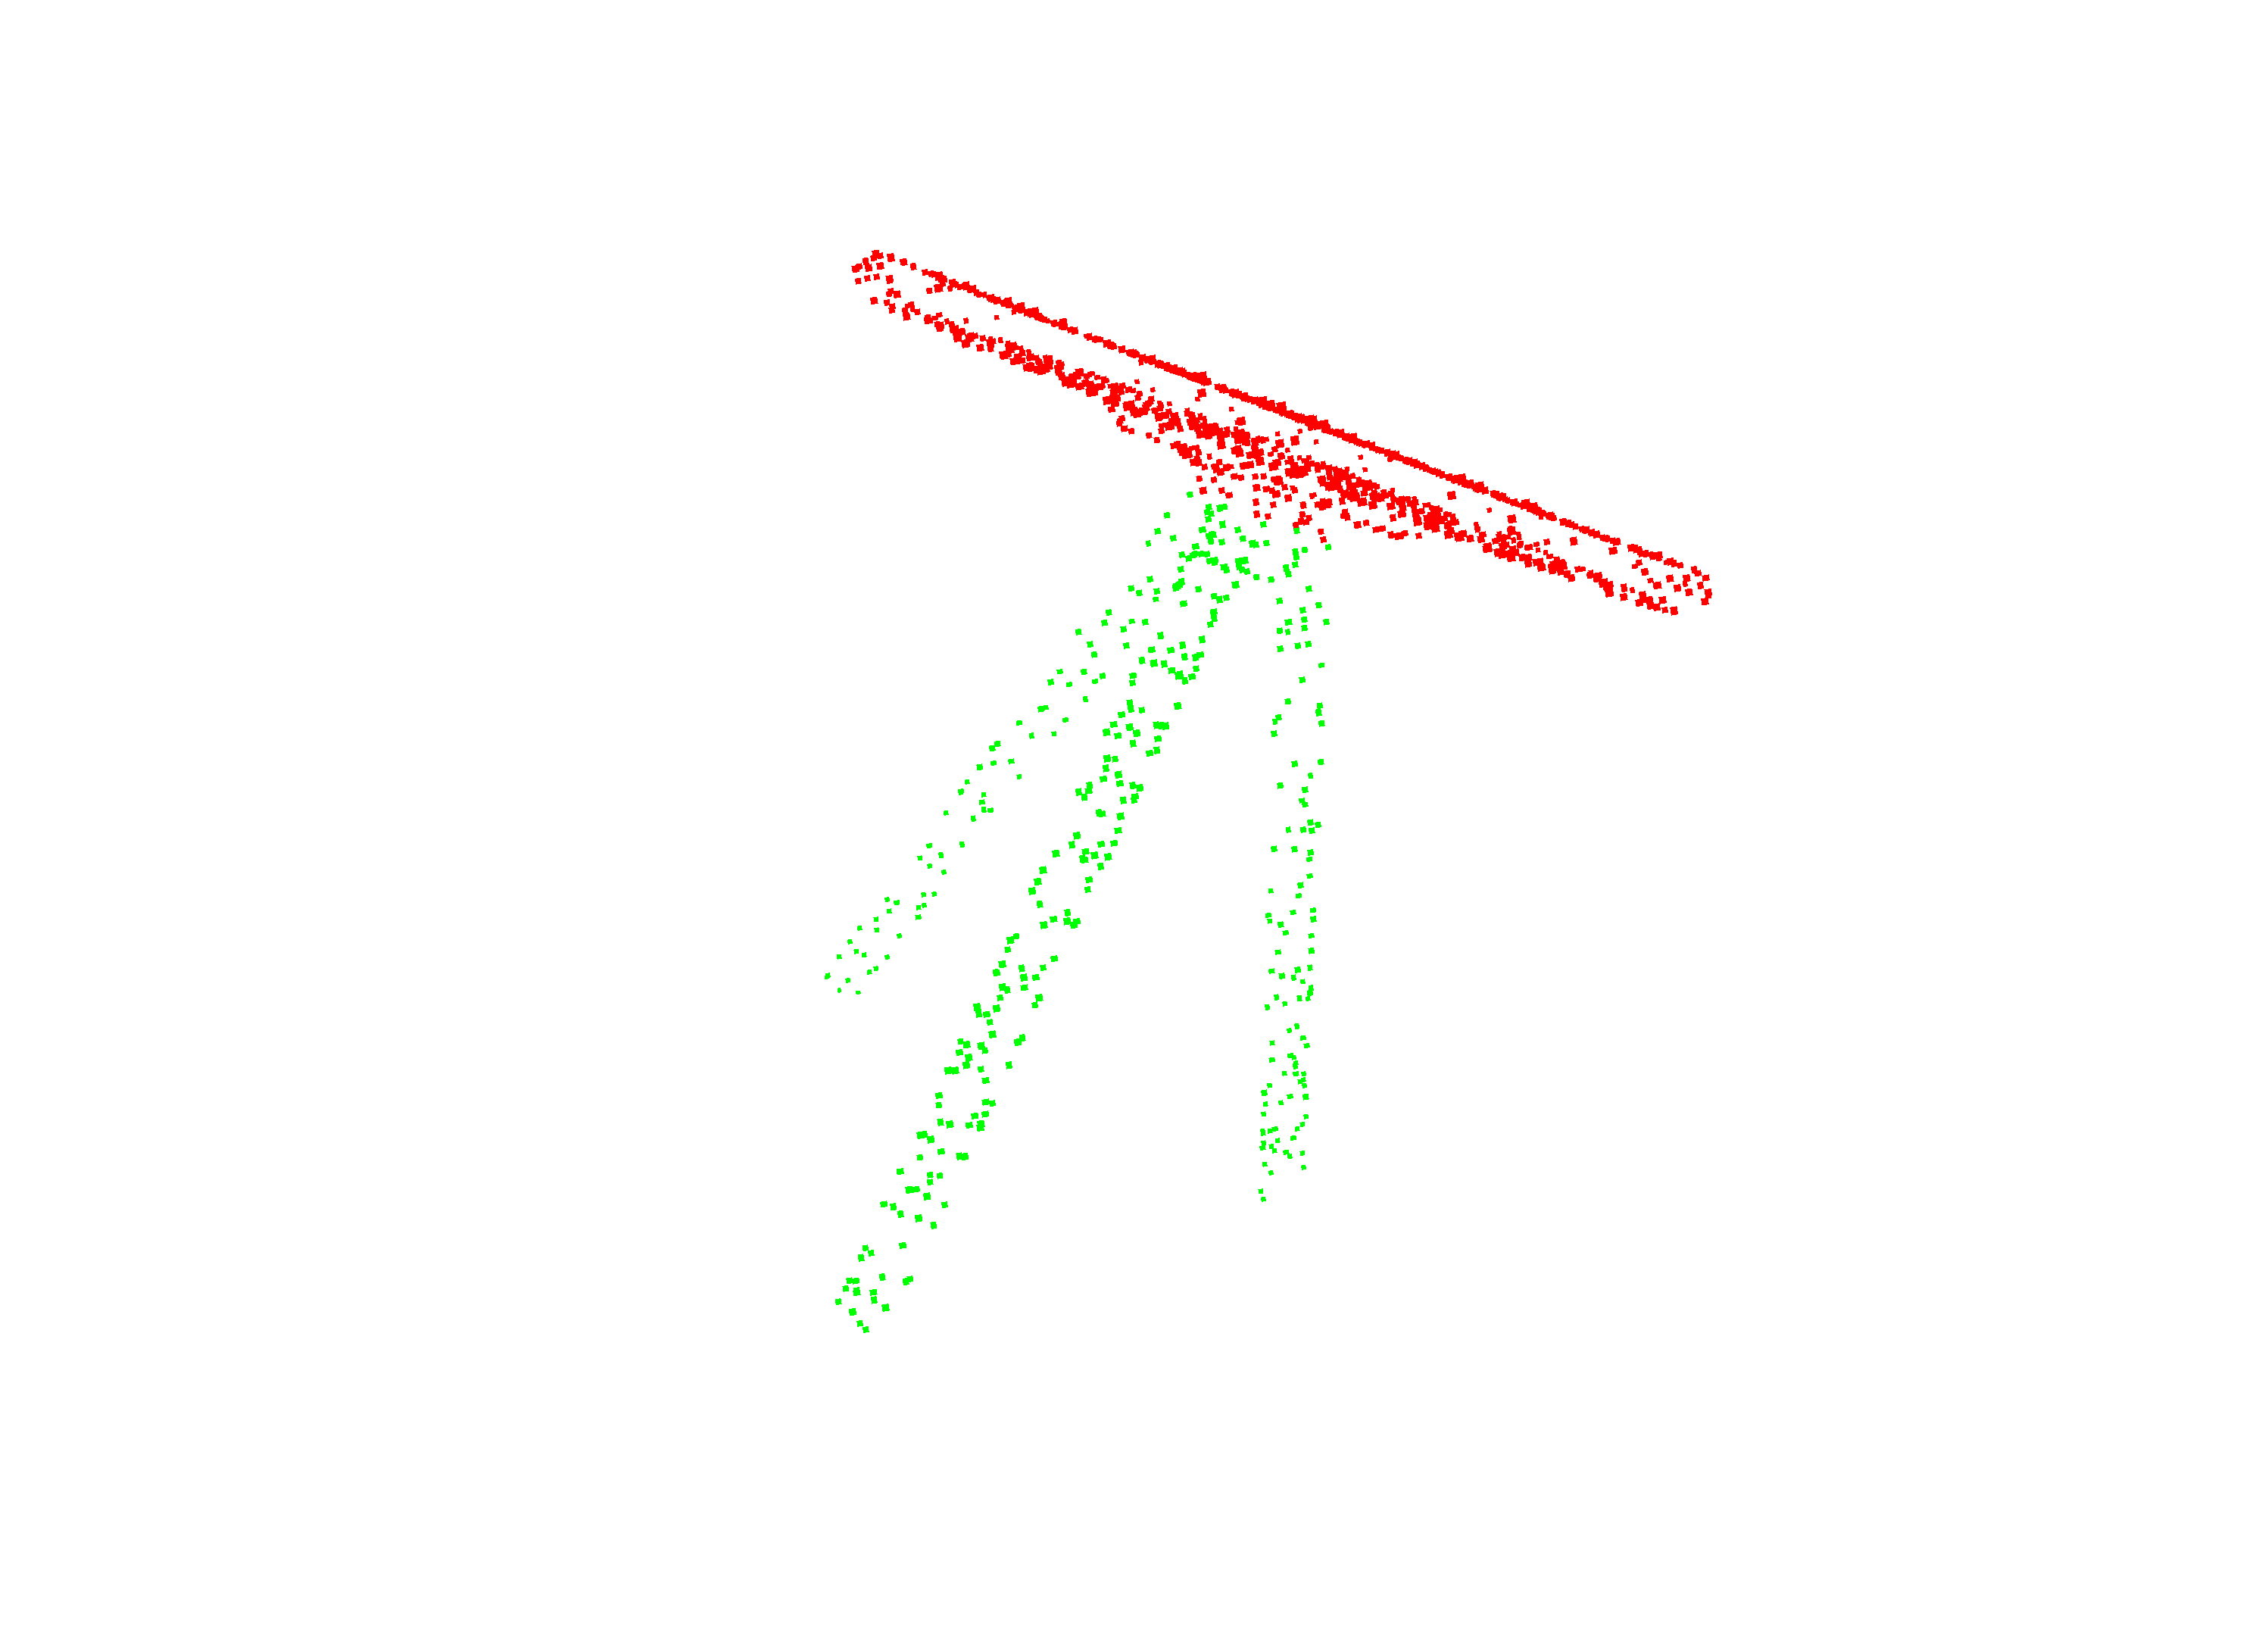
\includegraphics[width=\textwidth]{fig/supplement/part_segmentation/table/table02.pdf}
    \end{minipage}
    \hfill
    \caption{Qualitative results for part segmentation. We show our prediction projection images from three different viewpoints.}
    \label{fig:part_segmentation}
\end{figure*}



\begin{figure*}[htbp]
    \centering

    % 第一行左侧的竖排标签
    \begin{minipage}{0.09\textwidth}
        \centering
        Full
        Fine-tuning
    \end{minipage}
    \hfill
    % 第一行图片
    \begin{minipage}{0.22\textwidth}
        \centering
        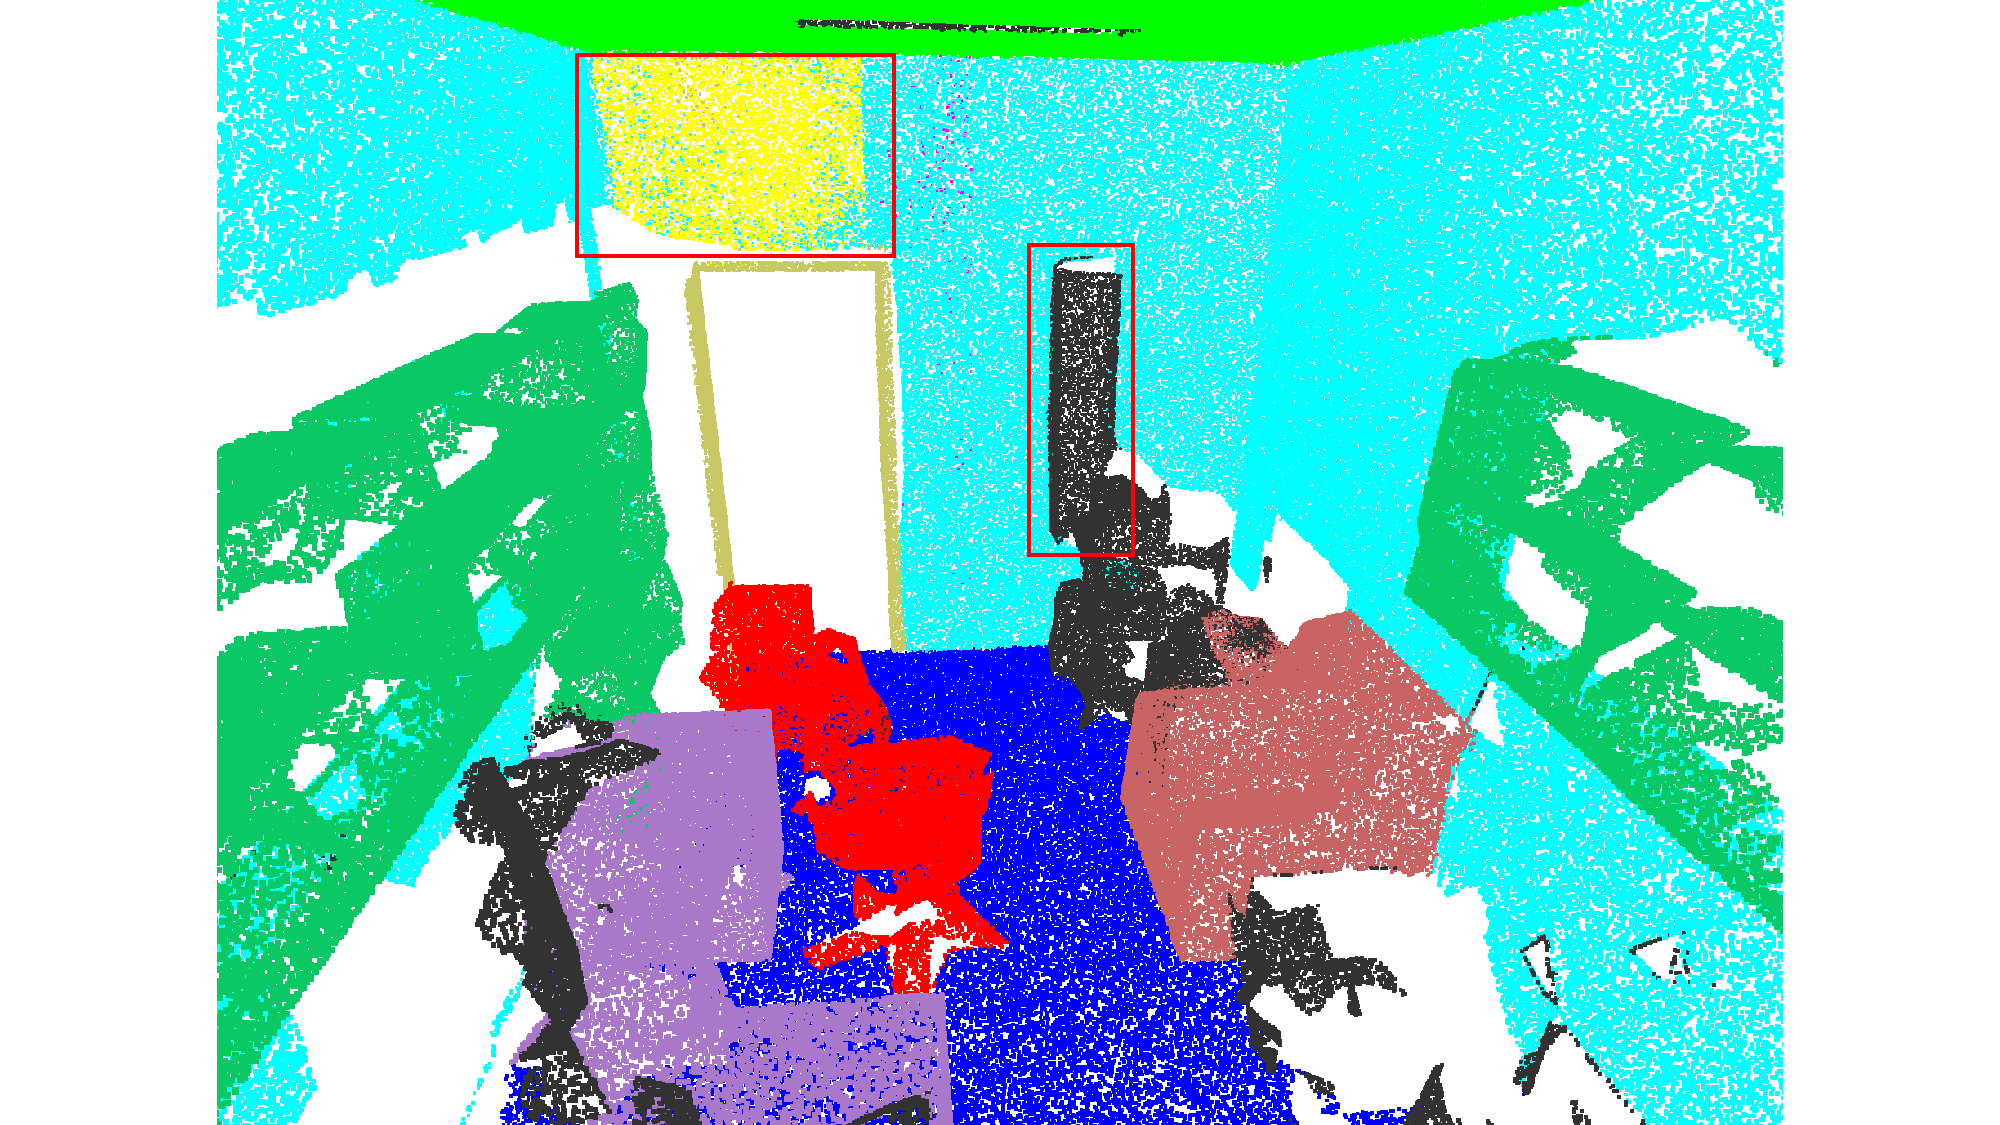
\includegraphics[width=\textwidth]{fig/supplement/semantic_segmentation/office_9/PT_office_9.pdf}
    \end{minipage}
    \hfill
    \begin{minipage}{0.22\textwidth}
        \centering
        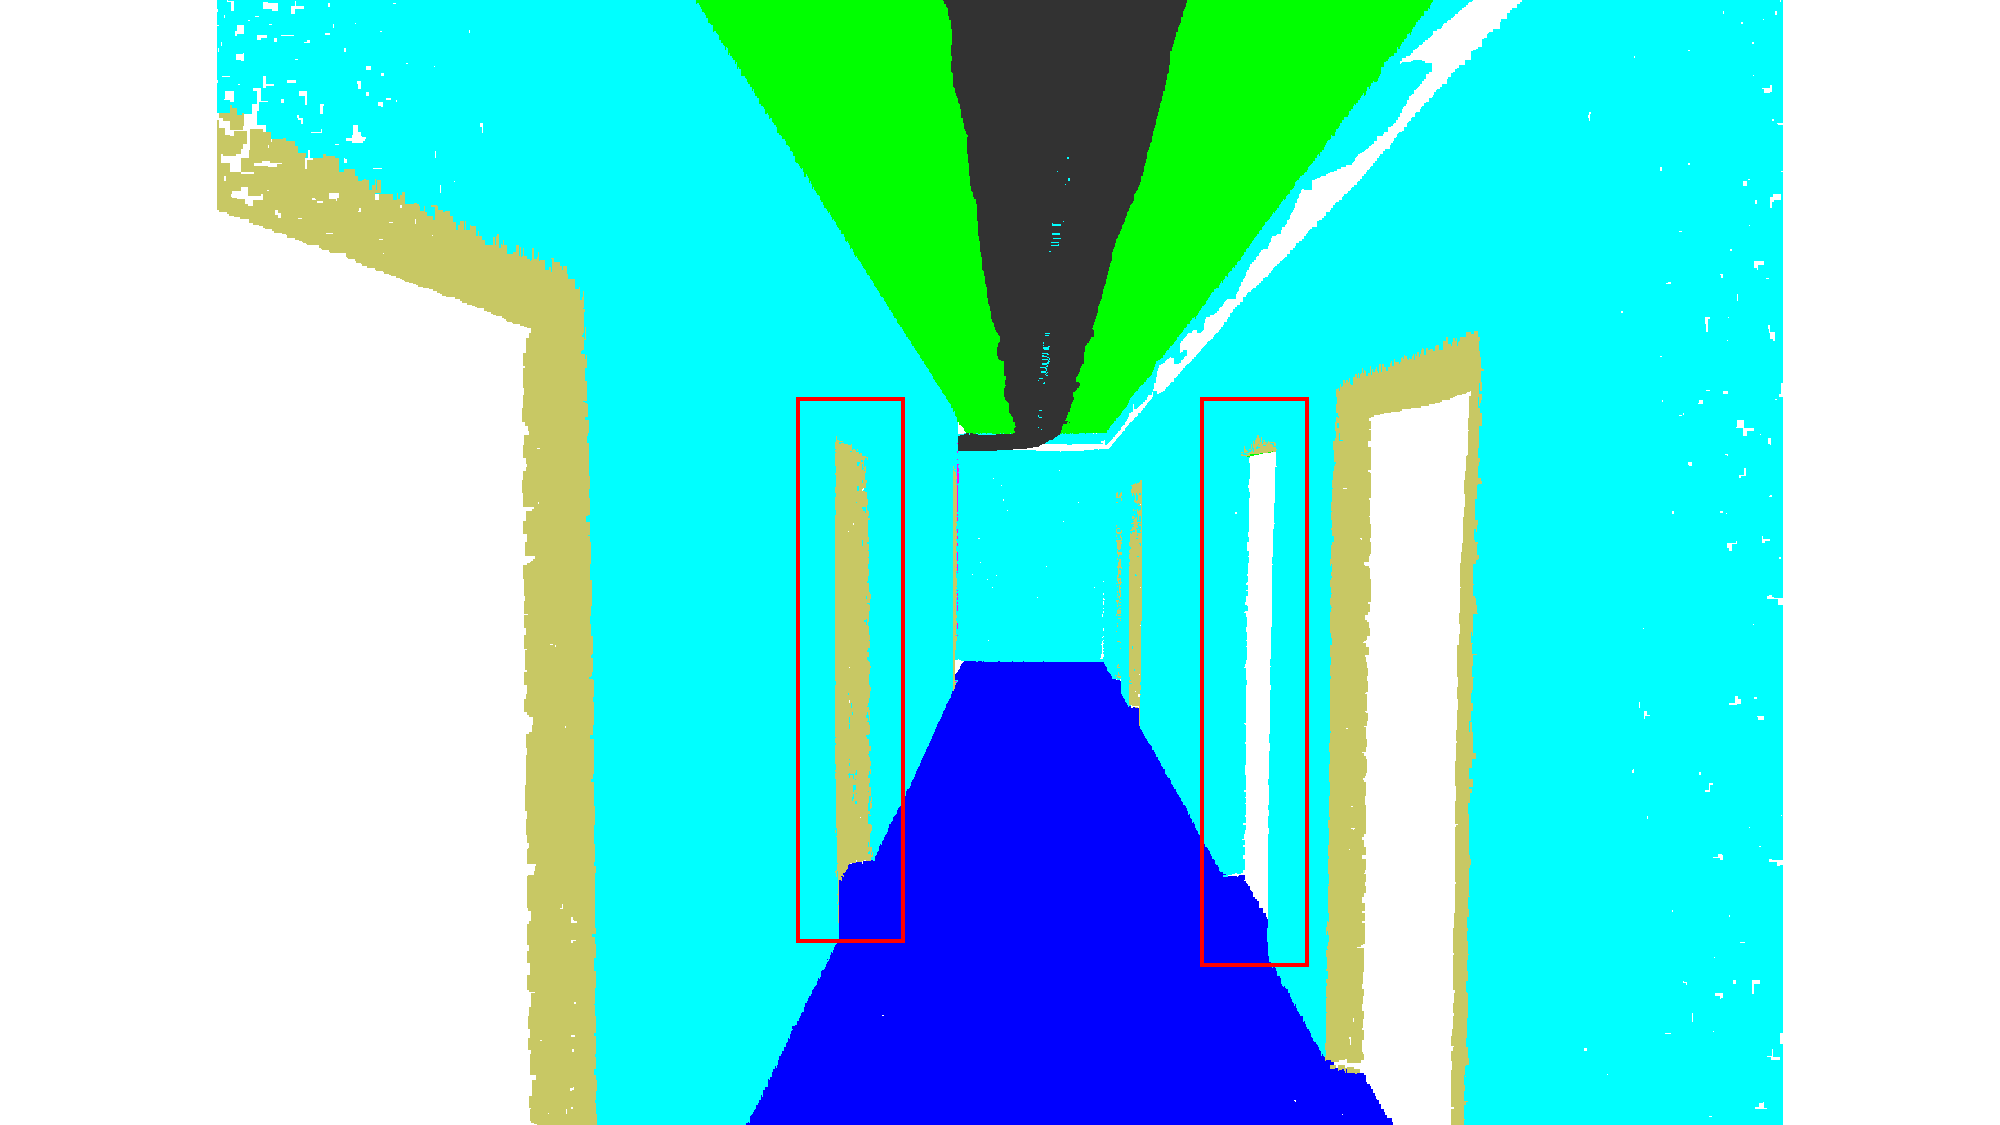
\includegraphics[width=\textwidth]{fig/supplement/semantic_segmentation/hallway_10/PT_hallway_10.pdf} % 替换为你的图片路径
    \end{minipage}
    \hfill
    \begin{minipage}{0.22\textwidth}
        \centering
        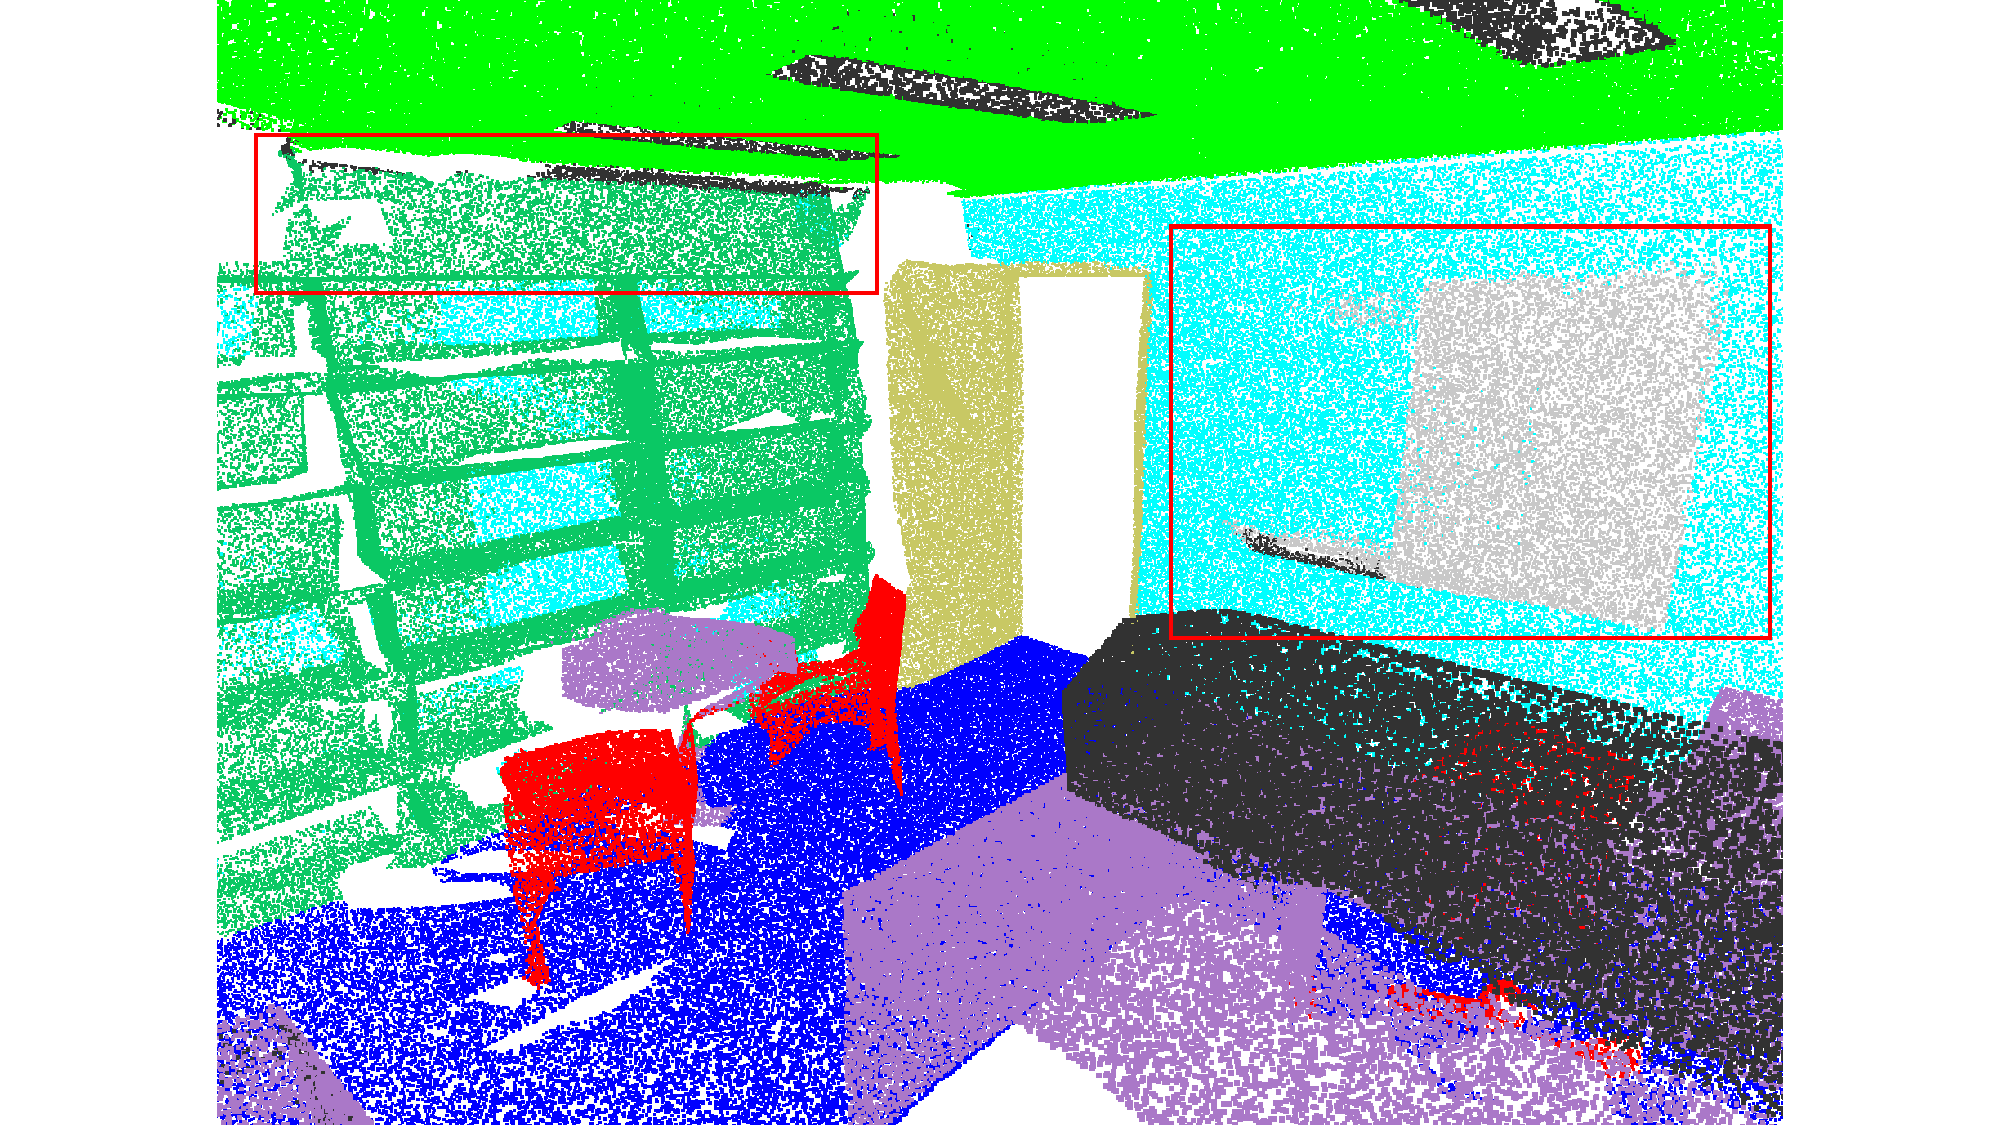
\includegraphics[width=\textwidth]{fig/supplement/semantic_segmentation/office_35/PT_office_35.pdf}
    \end{minipage}
    \hfill
    \begin{minipage}{0.22\textwidth}
        \centering
        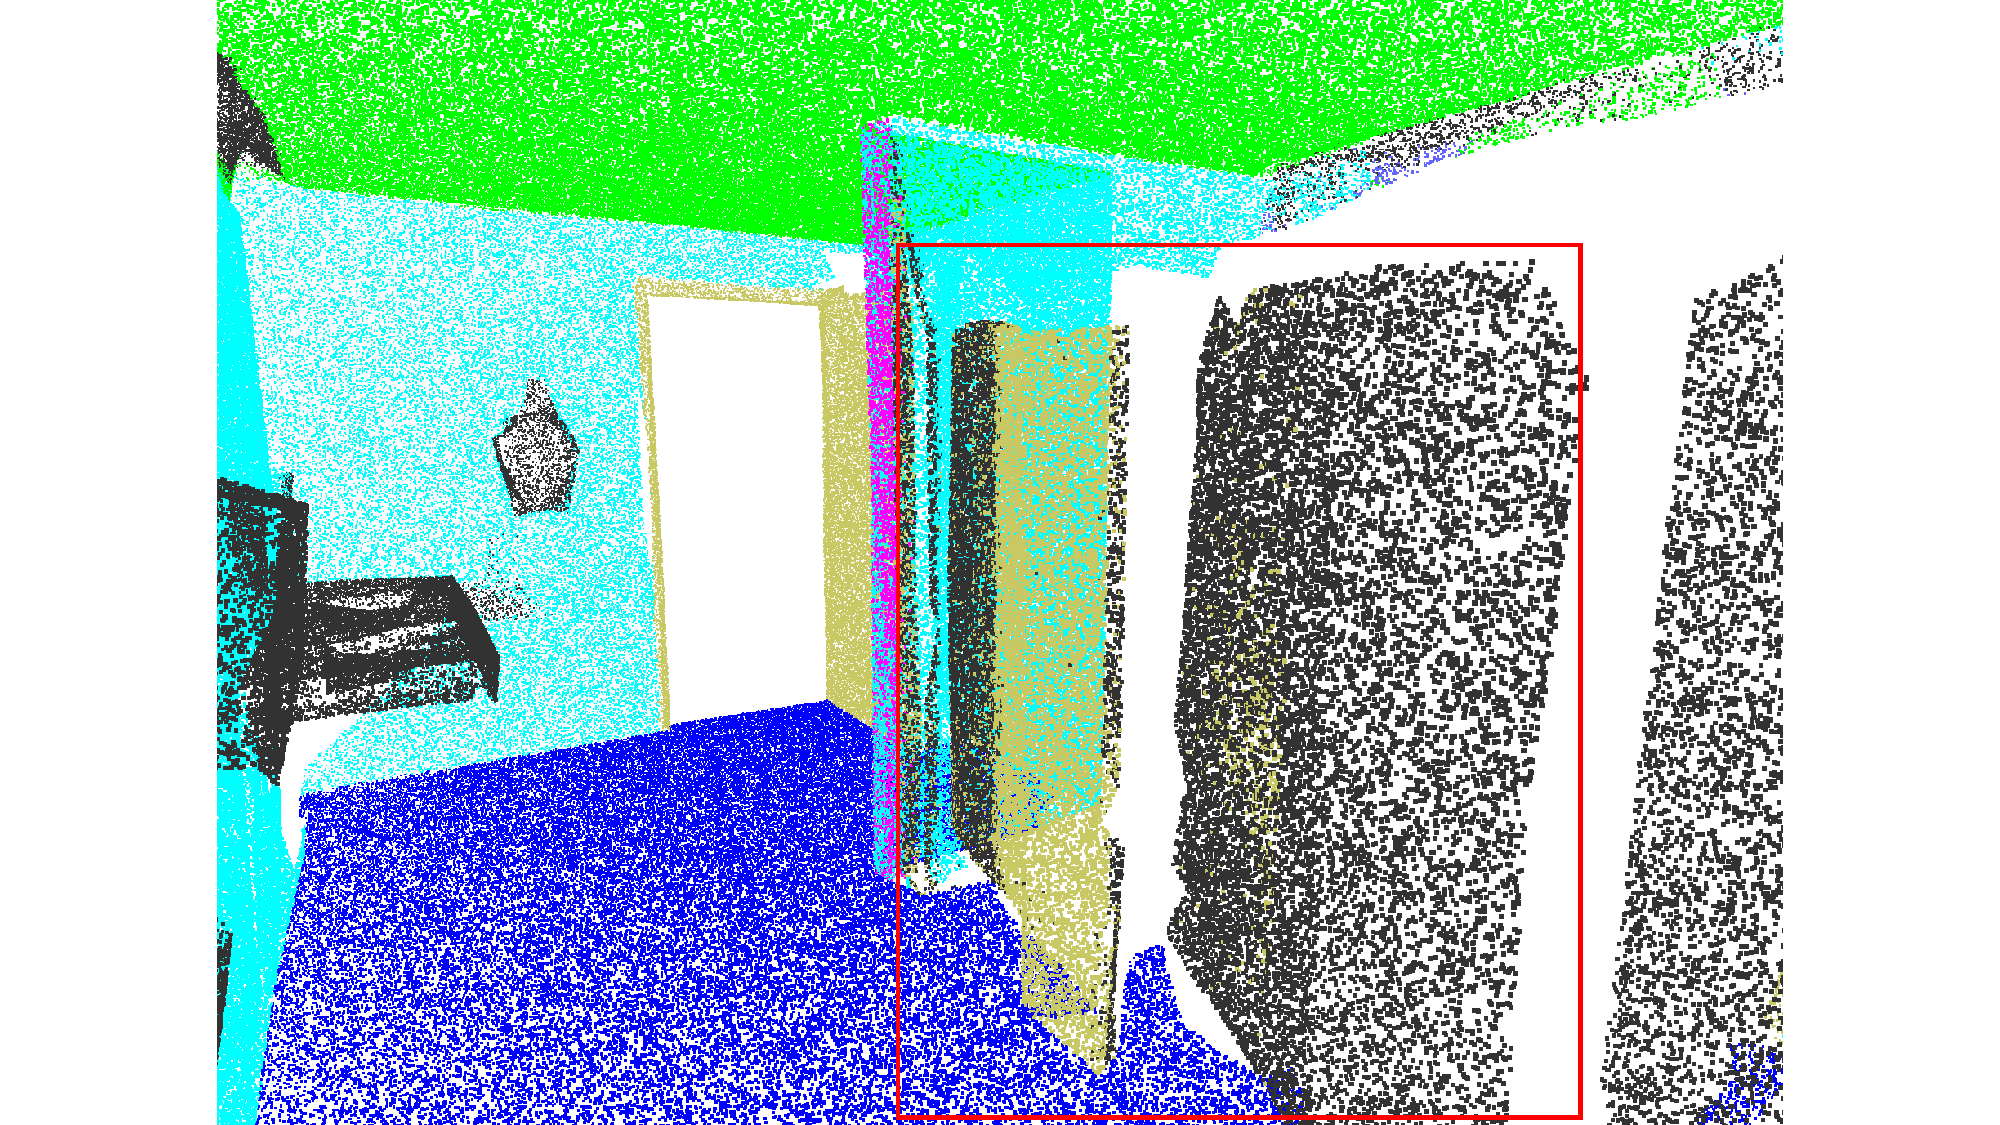
\includegraphics[width=\textwidth]{fig/supplement/semantic_segmentation/wc_2/PT_wc_2.pdf}
    \end{minipage}
    \hfill

    % 换行
    \vspace{0.5em}

    % 第二行左侧的竖排标签
    \begin{minipage}{0.09\textwidth}
        \centering
        DAPT
    \end{minipage}
    \hfill
    % 第二行图片
    \begin{minipage}{0.22\textwidth}
        \centering
        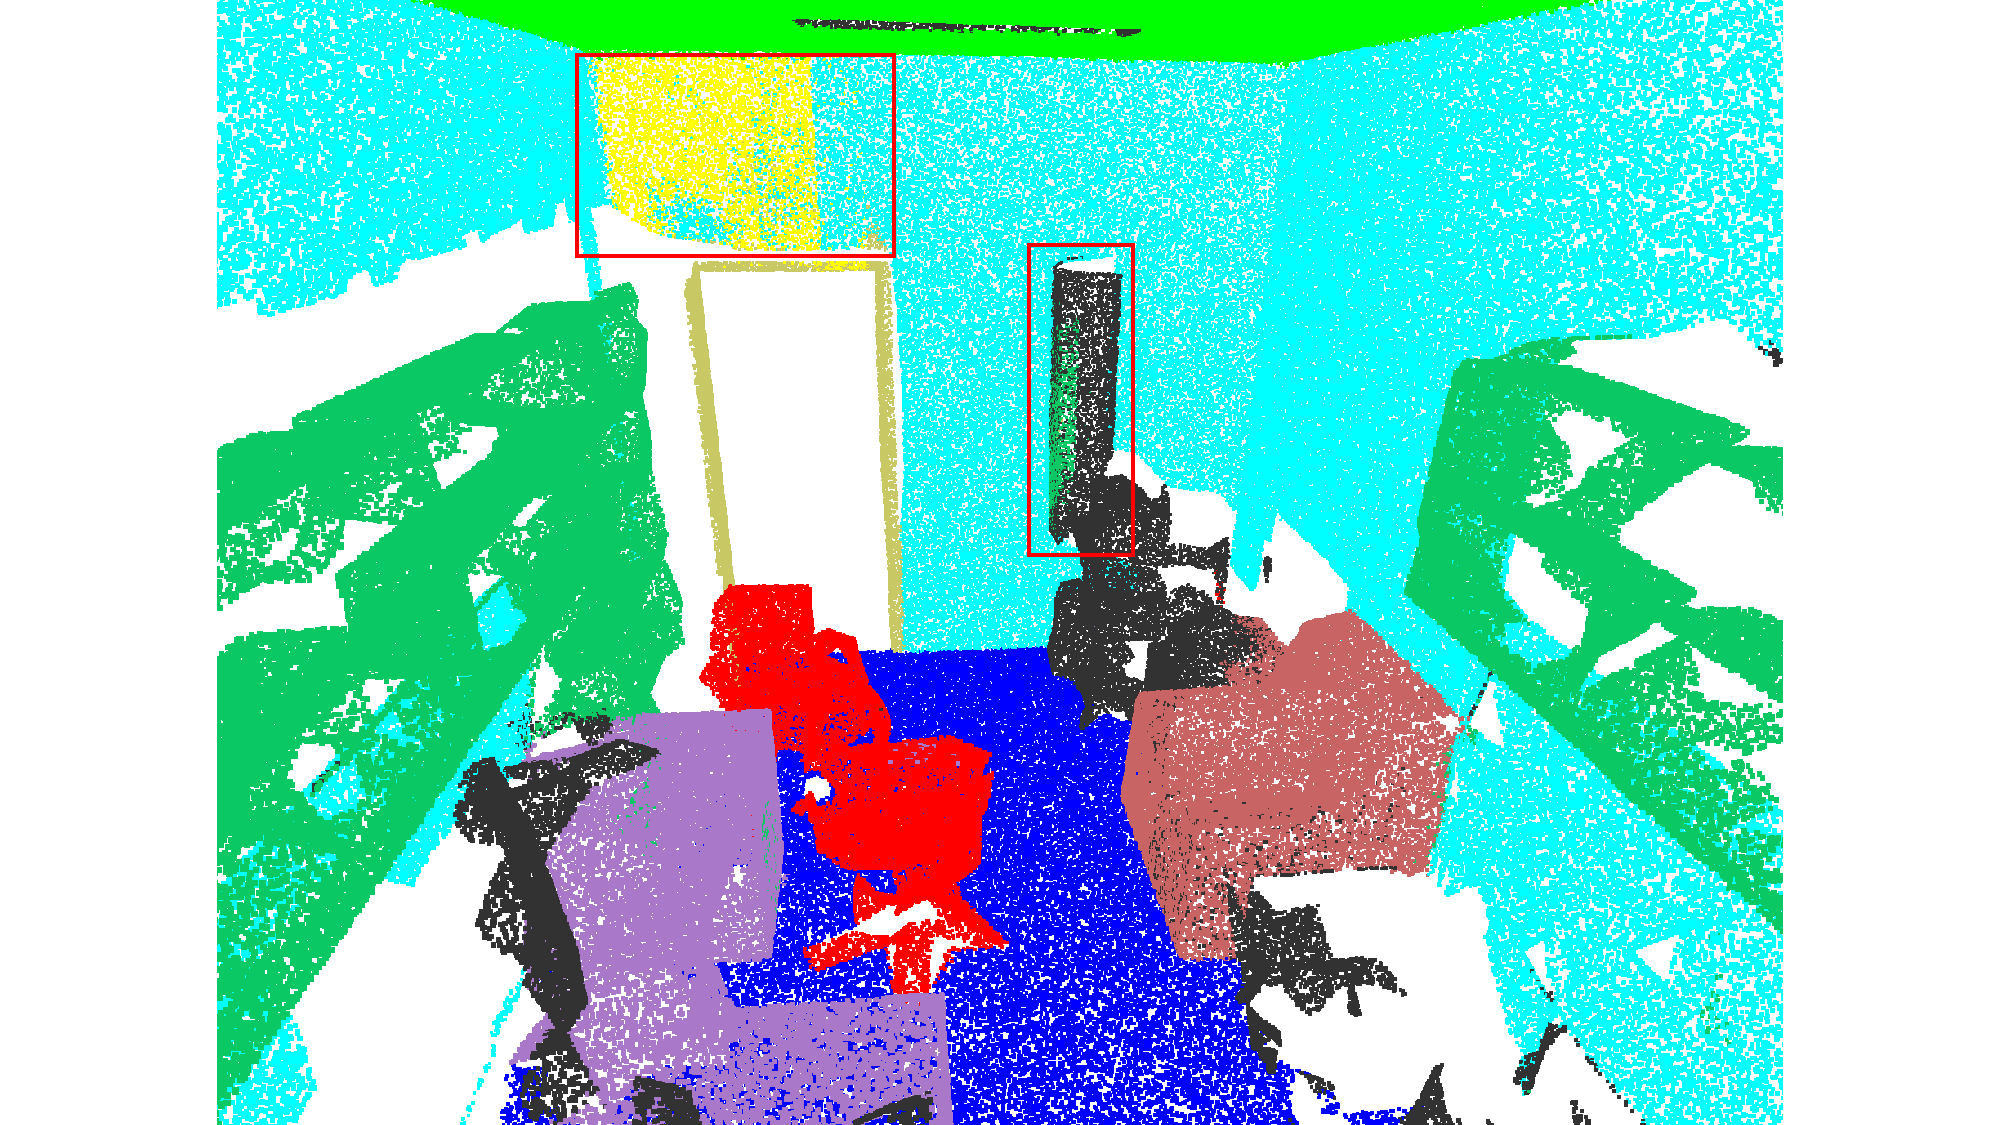
\includegraphics[width=\textwidth]{fig/supplement/semantic_segmentation/office_9/DAPT_office_9.pdf}
    \end{minipage}
    \hfill
    \begin{minipage}{0.22\textwidth}
        \centering
        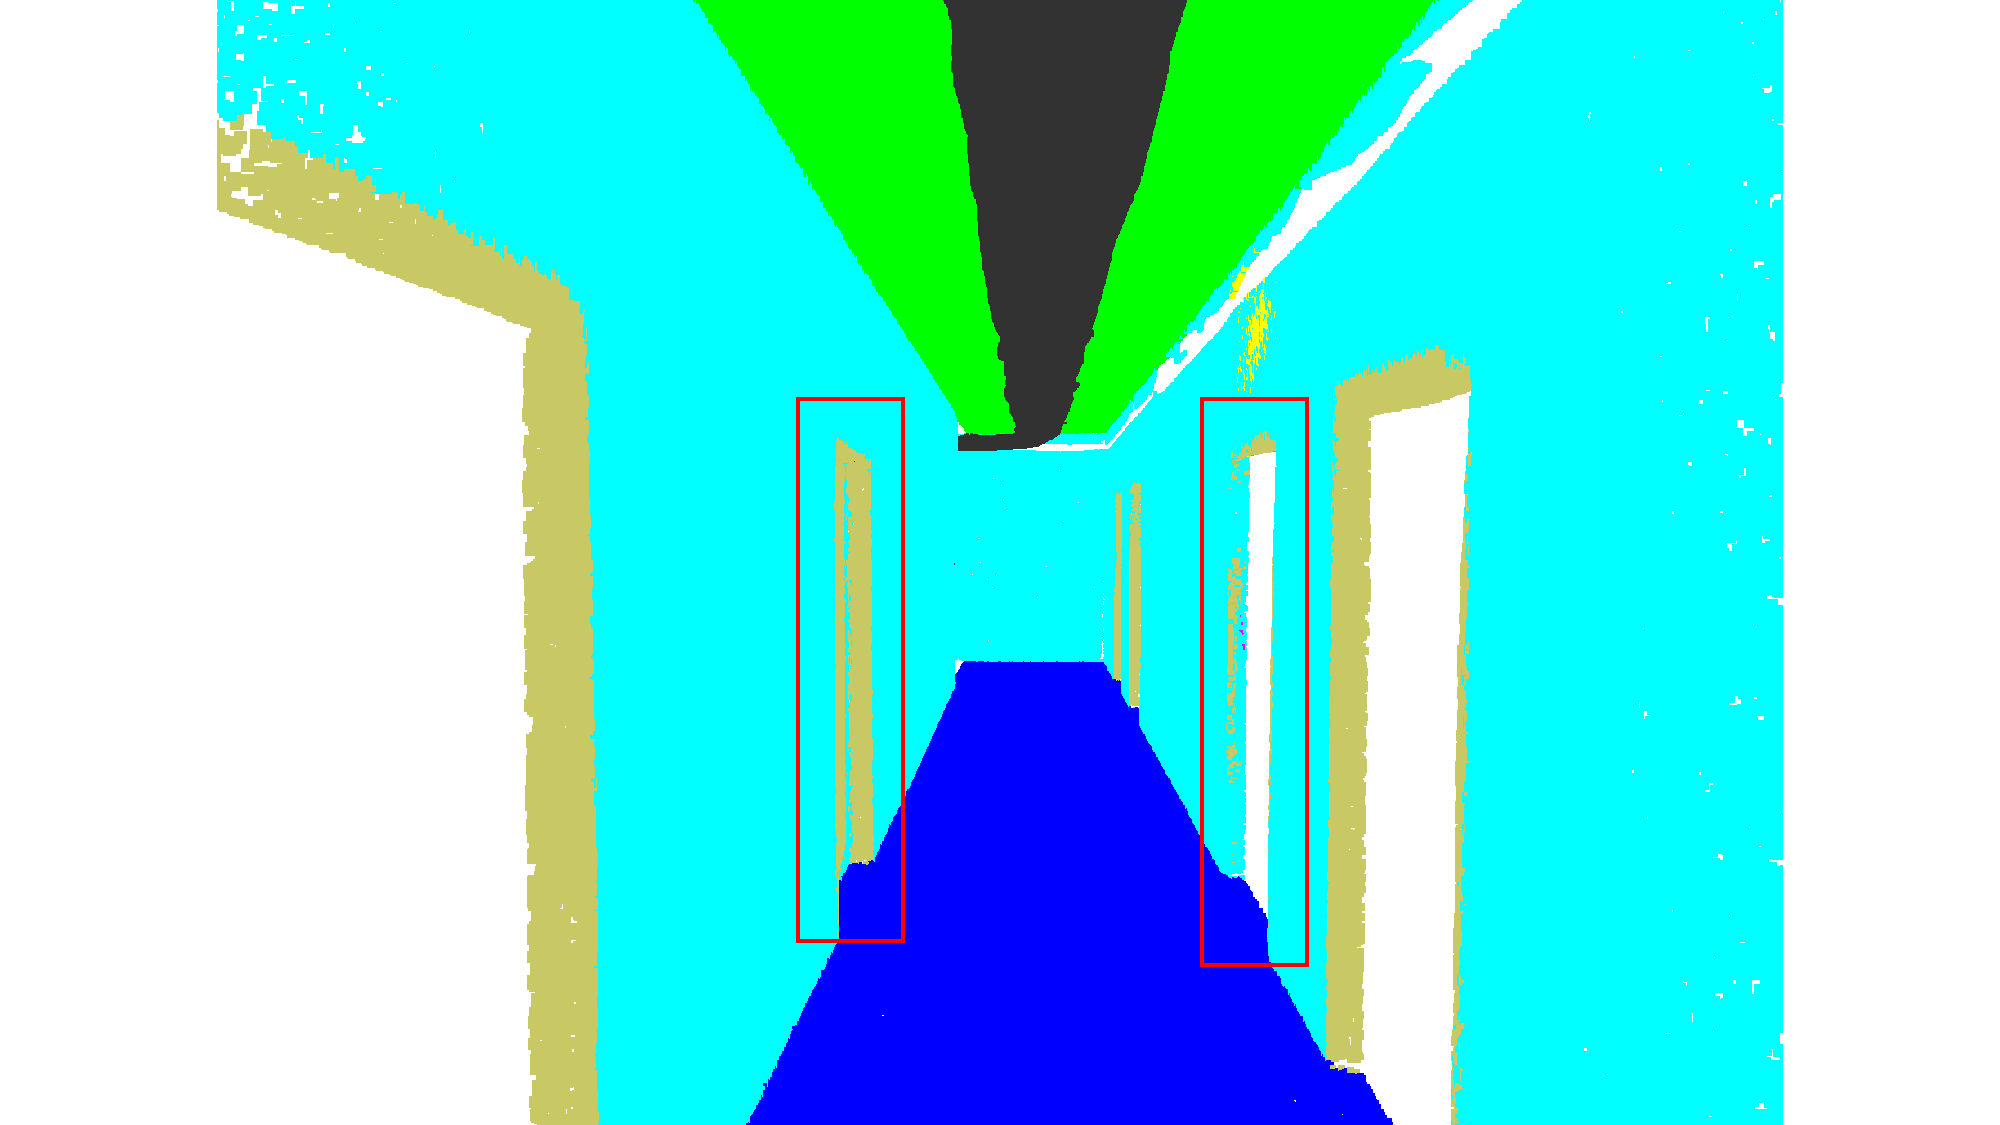
\includegraphics[width=\textwidth]{fig/supplement/semantic_segmentation/hallway_10/DAPT_hallway_10.pdf}
    \end{minipage}
    \hfill
    \begin{minipage}{0.22\textwidth}
        \centering
        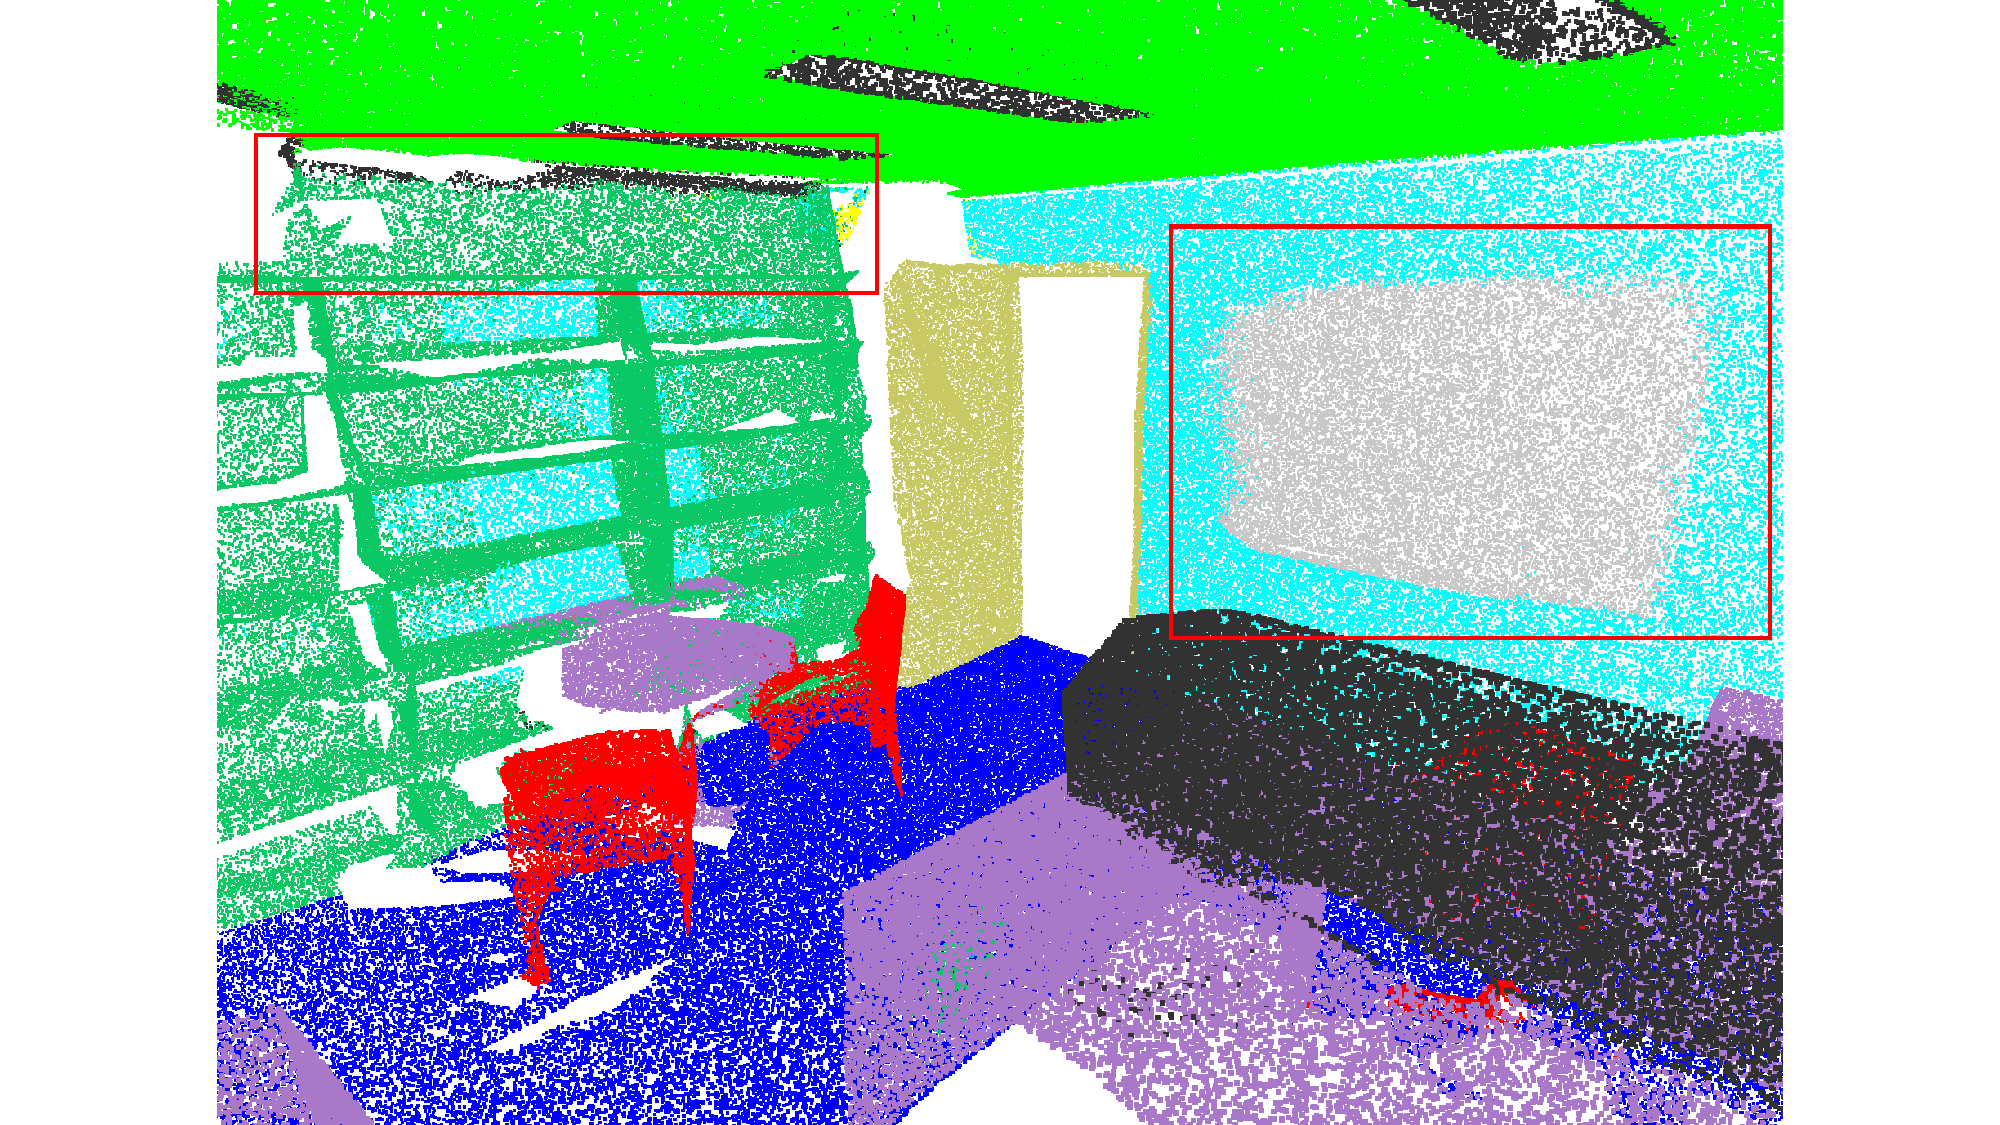
\includegraphics[width=\textwidth]{fig/supplement/semantic_segmentation/office_35/DAPT_office_35.pdf}
    \end{minipage}
    \hfill
    \begin{minipage}{0.22\textwidth}
        \centering
        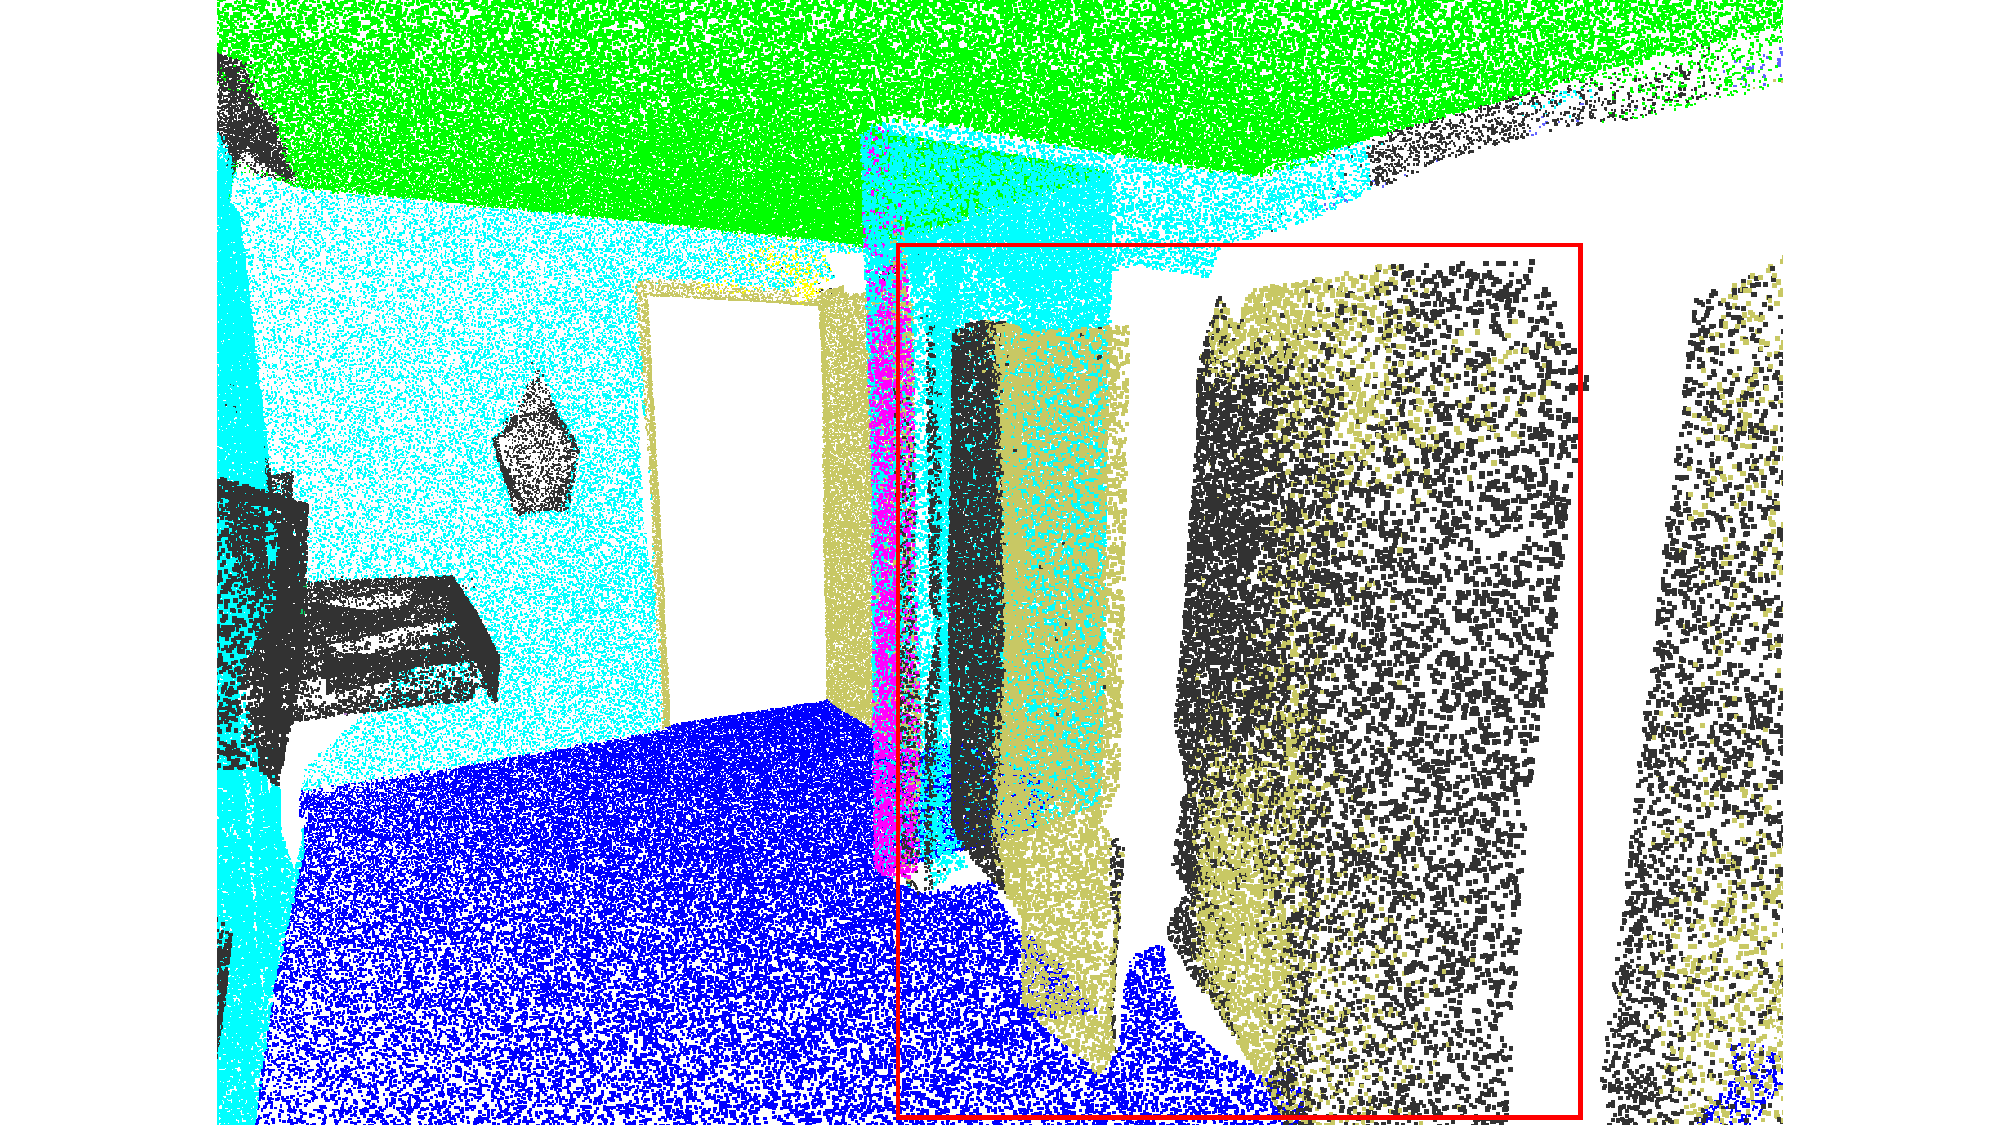
\includegraphics[width=\textwidth]{fig/supplement/semantic_segmentation/wc_2/DAPT_wc_2.pdf}
    \end{minipage}
    \hfill

    % 换行
    \vspace{0.5em}

    % 第三行左侧的竖排标签
    \begin{minipage}{0.09\textwidth}
        \centering
        IDPT
    \end{minipage}
    \hfill
    % 第三行图片
    \begin{minipage}{0.22\textwidth}
        \centering
        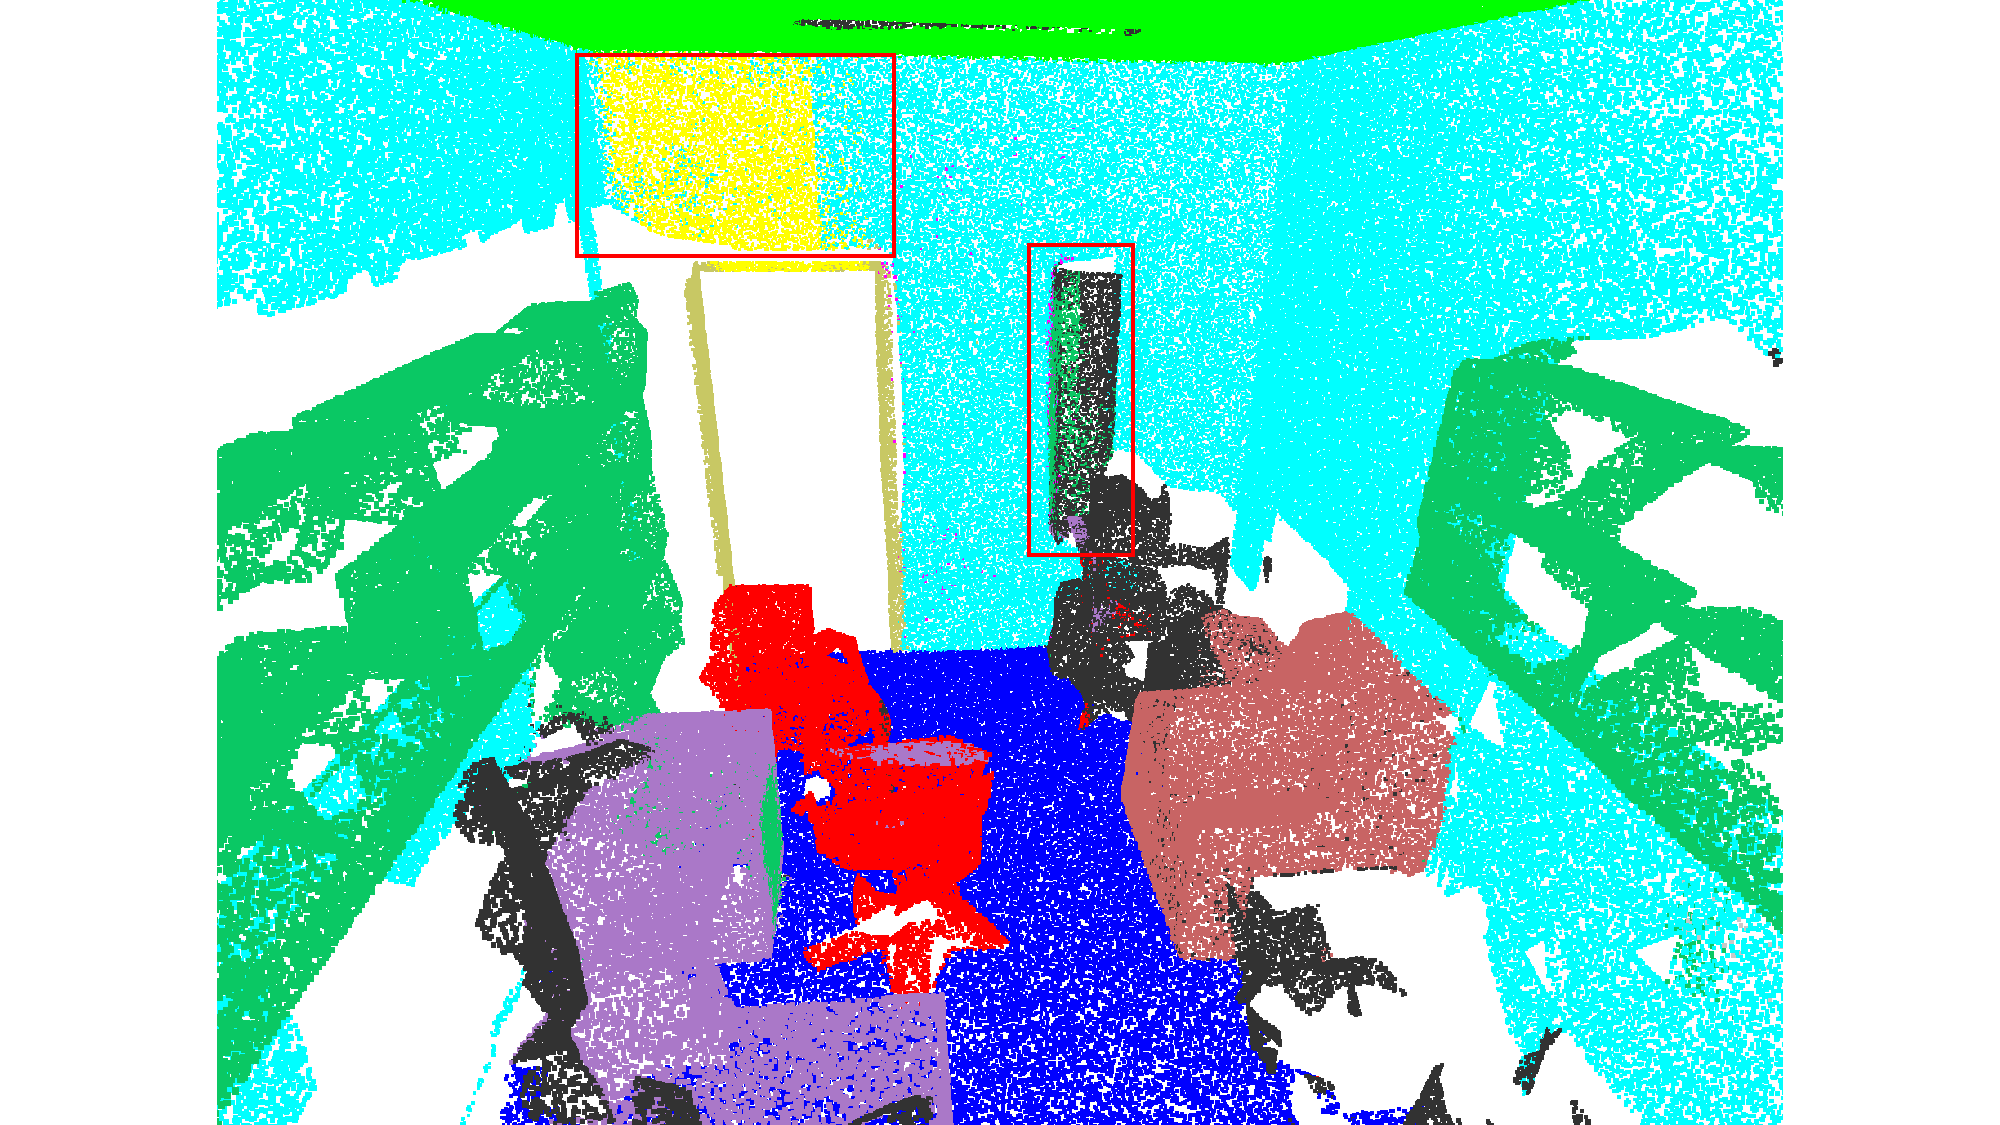
\includegraphics[width=\textwidth]{fig/supplement/semantic_segmentation/office_9/IDPT_office_9.pdf}
    \end{minipage}
    \hfill
    \begin{minipage}{0.22\textwidth}
        \centering
        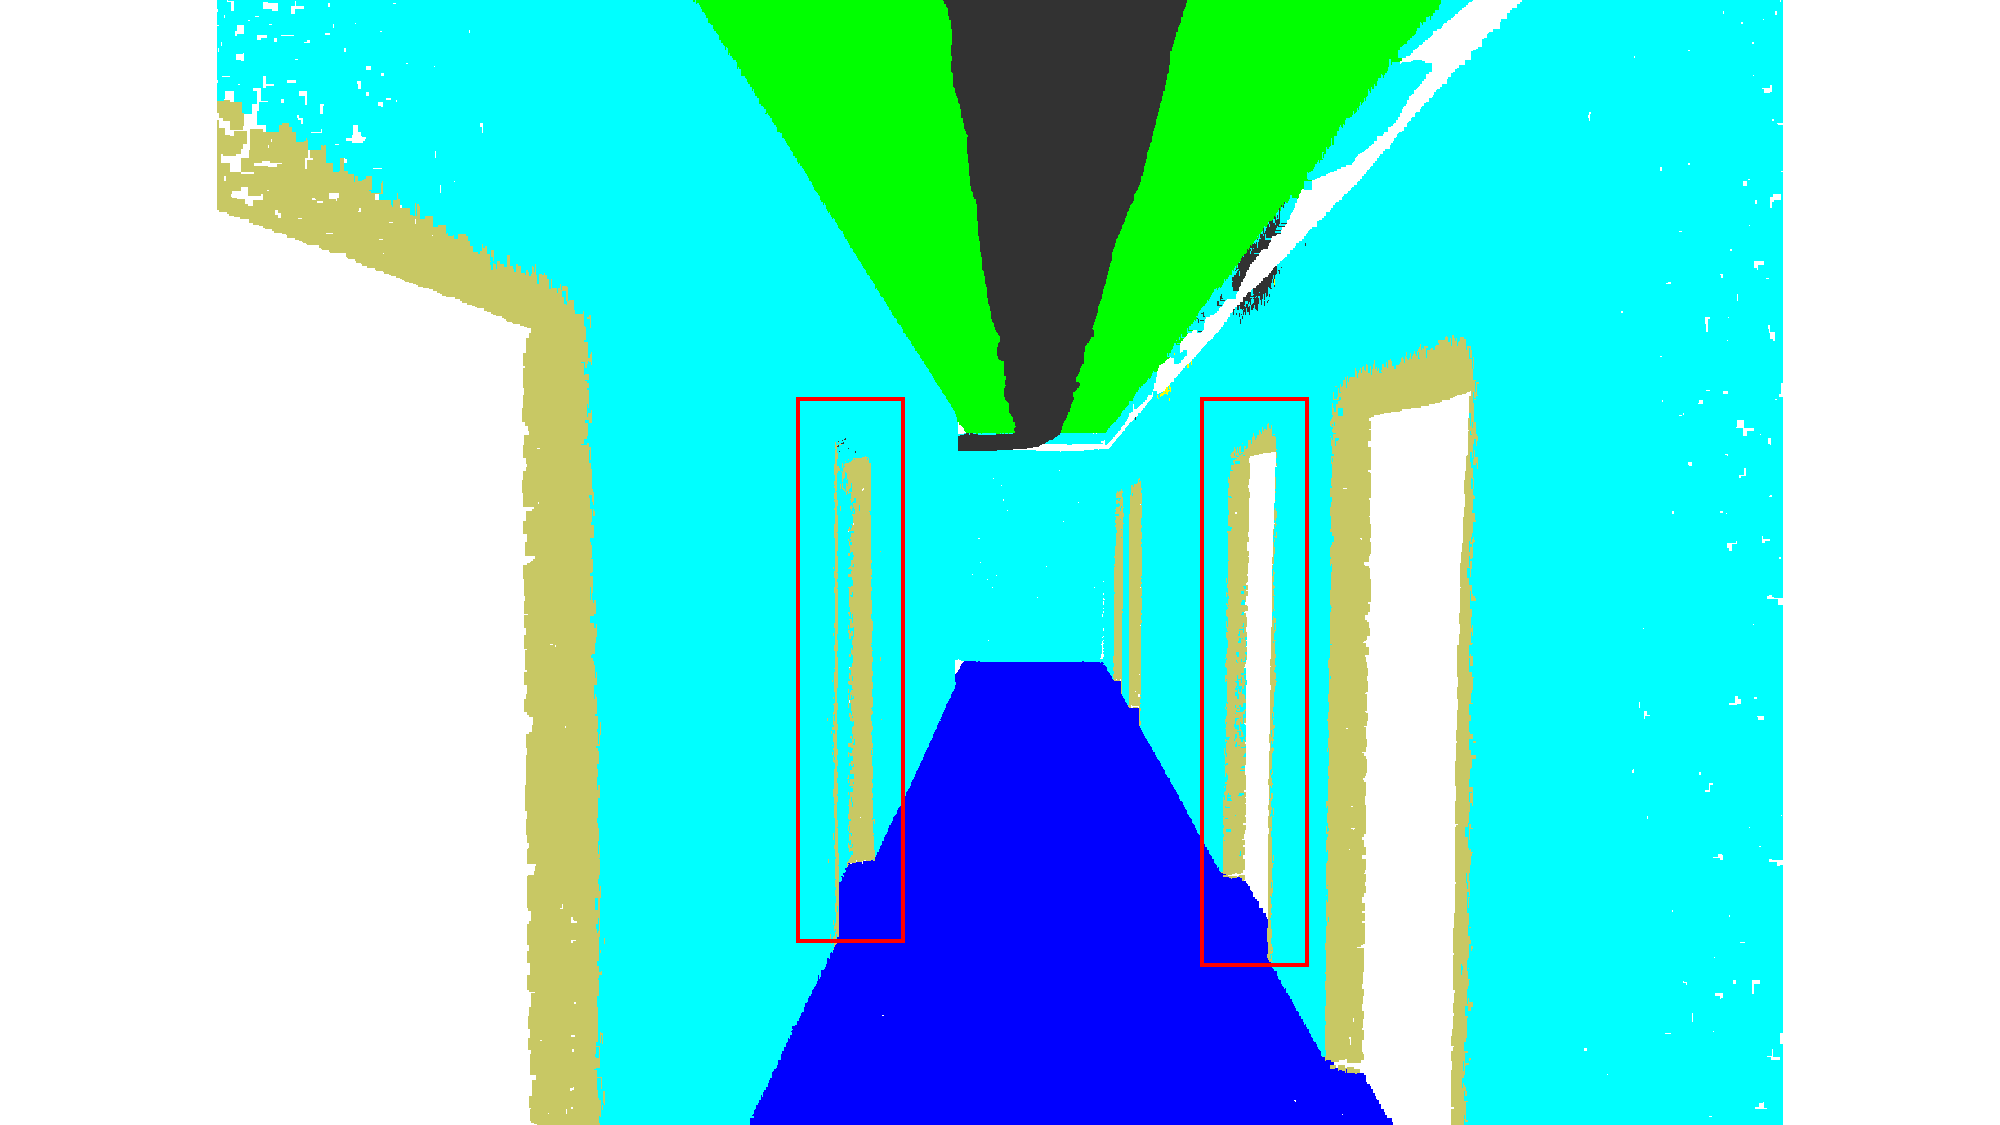
\includegraphics[width=\textwidth]{fig/supplement/semantic_segmentation/hallway_10/IDPT_hallway_10.pdf}
    \end{minipage}
    \hfill
    \begin{minipage}{0.22\textwidth}
        \centering
        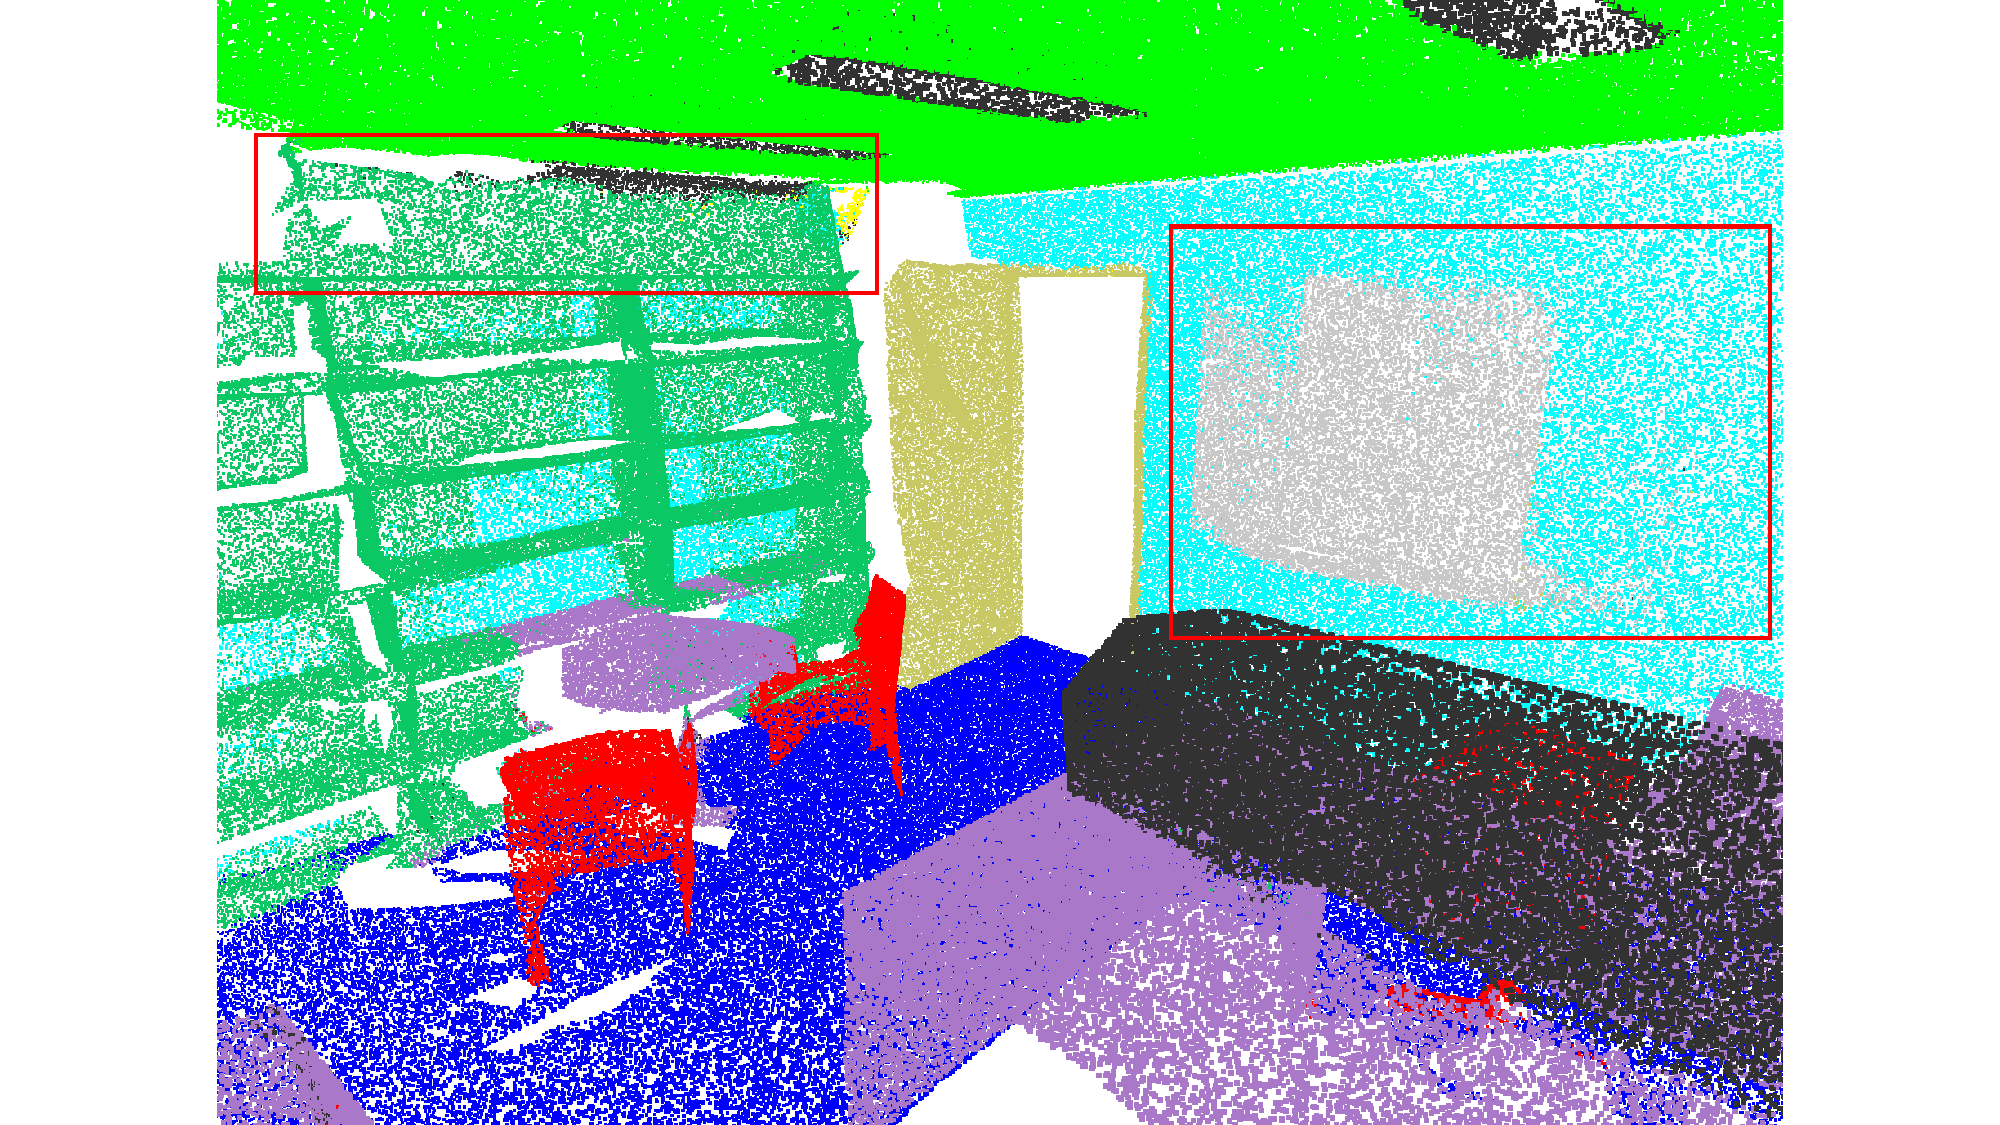
\includegraphics[width=\textwidth]{fig/supplement/semantic_segmentation/office_35/IDPT_office_35.pdf}
    \end{minipage}
    \hfill
    \begin{minipage}{0.22\textwidth}
        \centering
        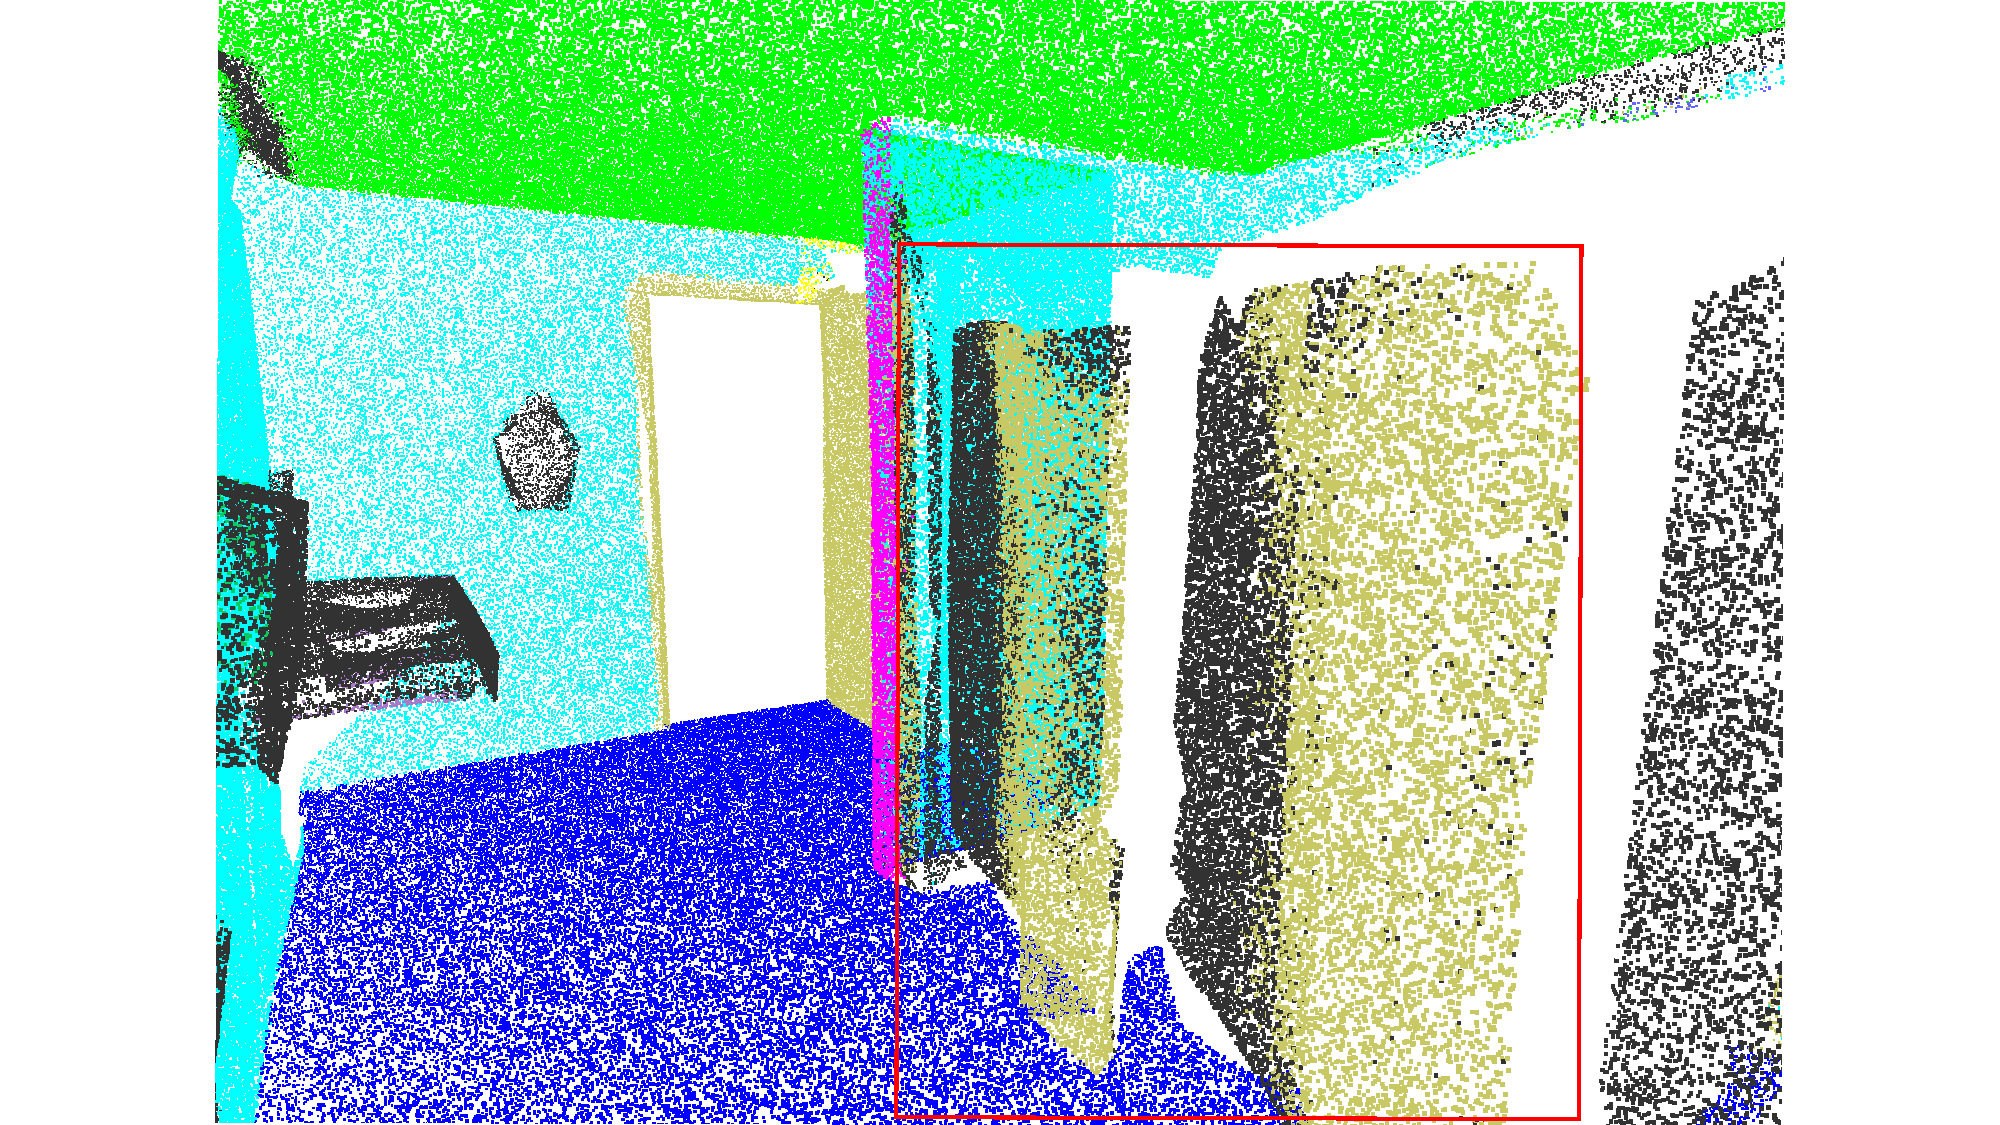
\includegraphics[width=\textwidth]{fig/supplement/semantic_segmentation/wc_2/IDPT_wc_2.pdf}
    \end{minipage}
    \hfill

    % 换行
    \vspace{0.5em}

    % 第四行左侧的竖排标签
    \begin{minipage}{0.09\textwidth}
        \centering
        PPT
    \end{minipage}
    \hfill
    % 第四行图片
    \begin{minipage}{0.22\textwidth}
        \centering
        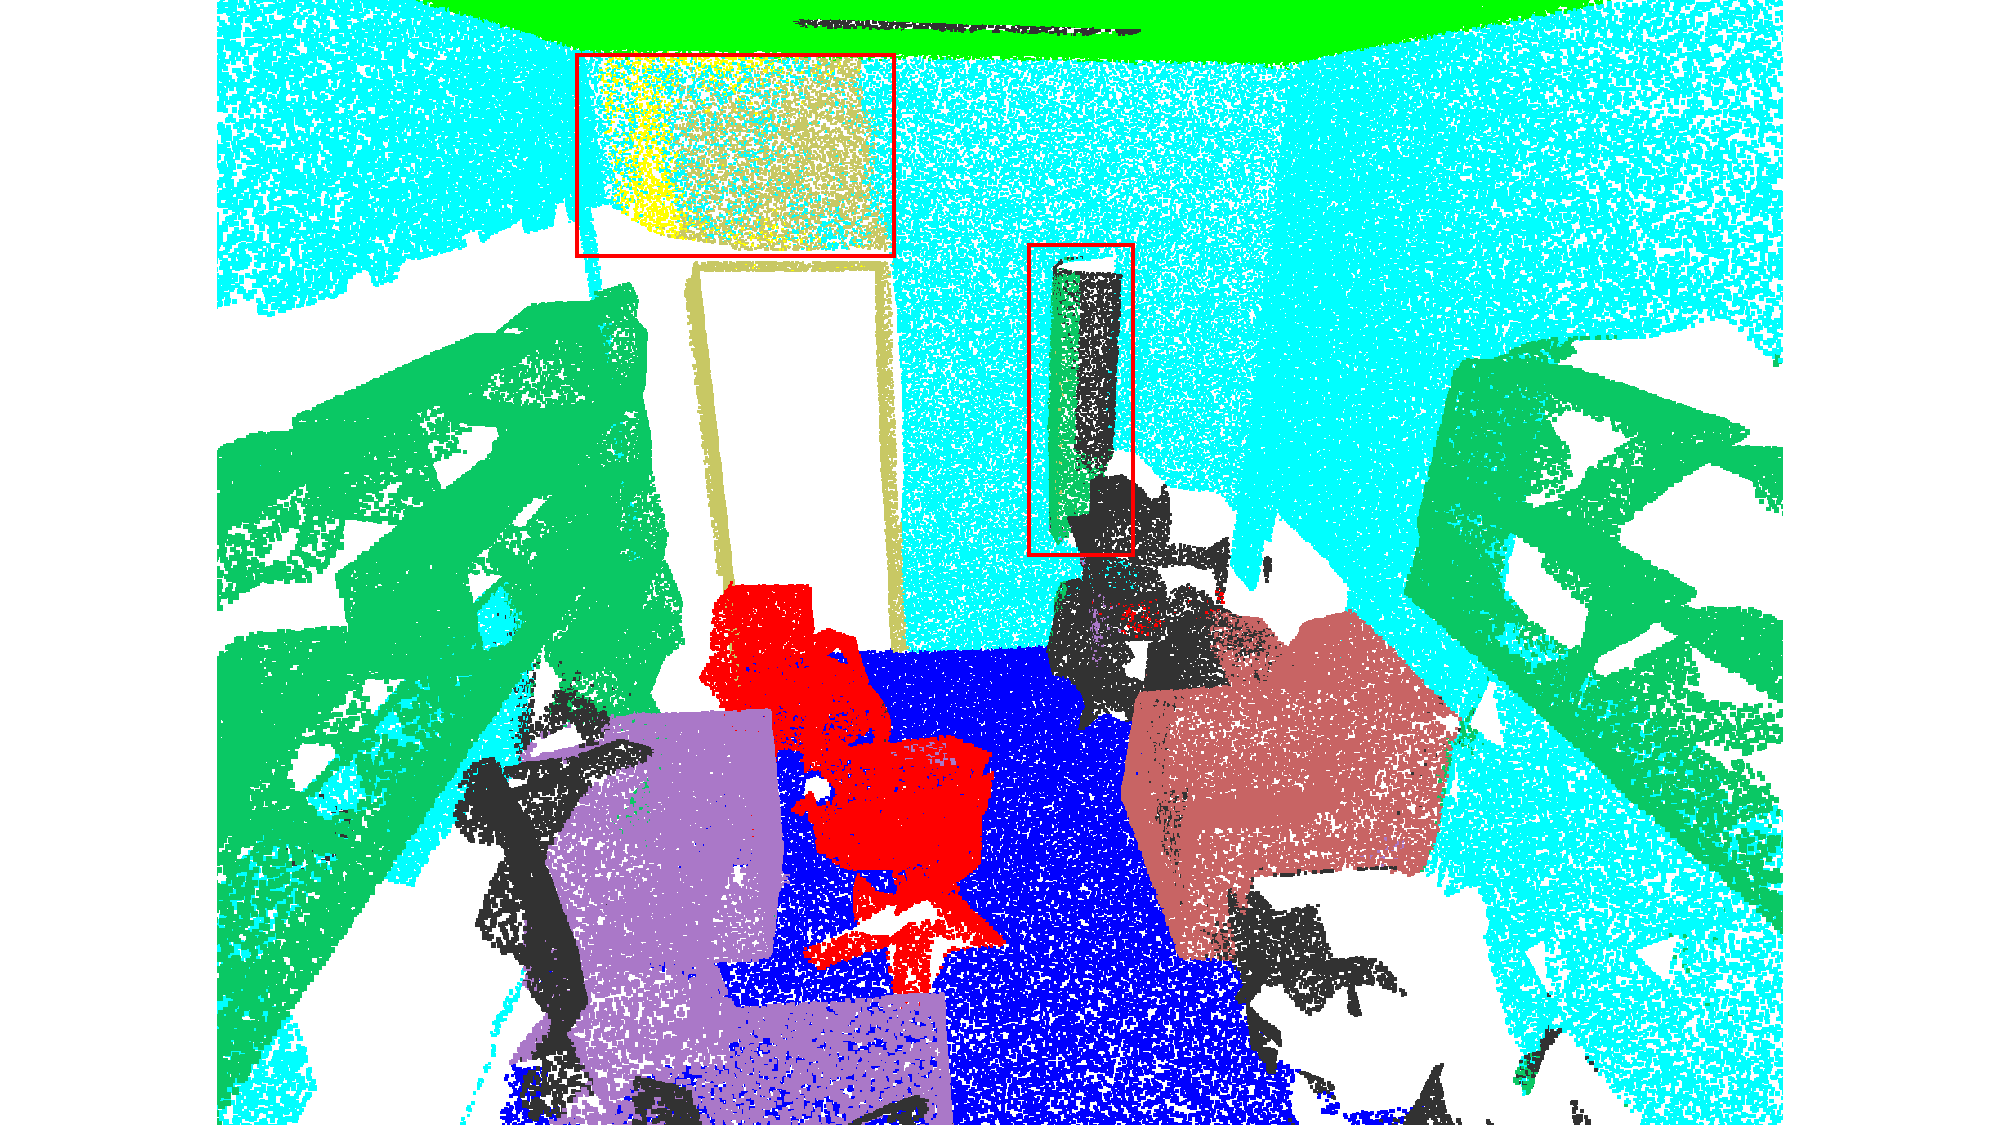
\includegraphics[width=\textwidth]{fig/supplement/semantic_segmentation/office_9/PPT_office_9.pdf}
    \end{minipage}
    \hfill
     \begin{minipage}{0.22\textwidth}
        \centering
        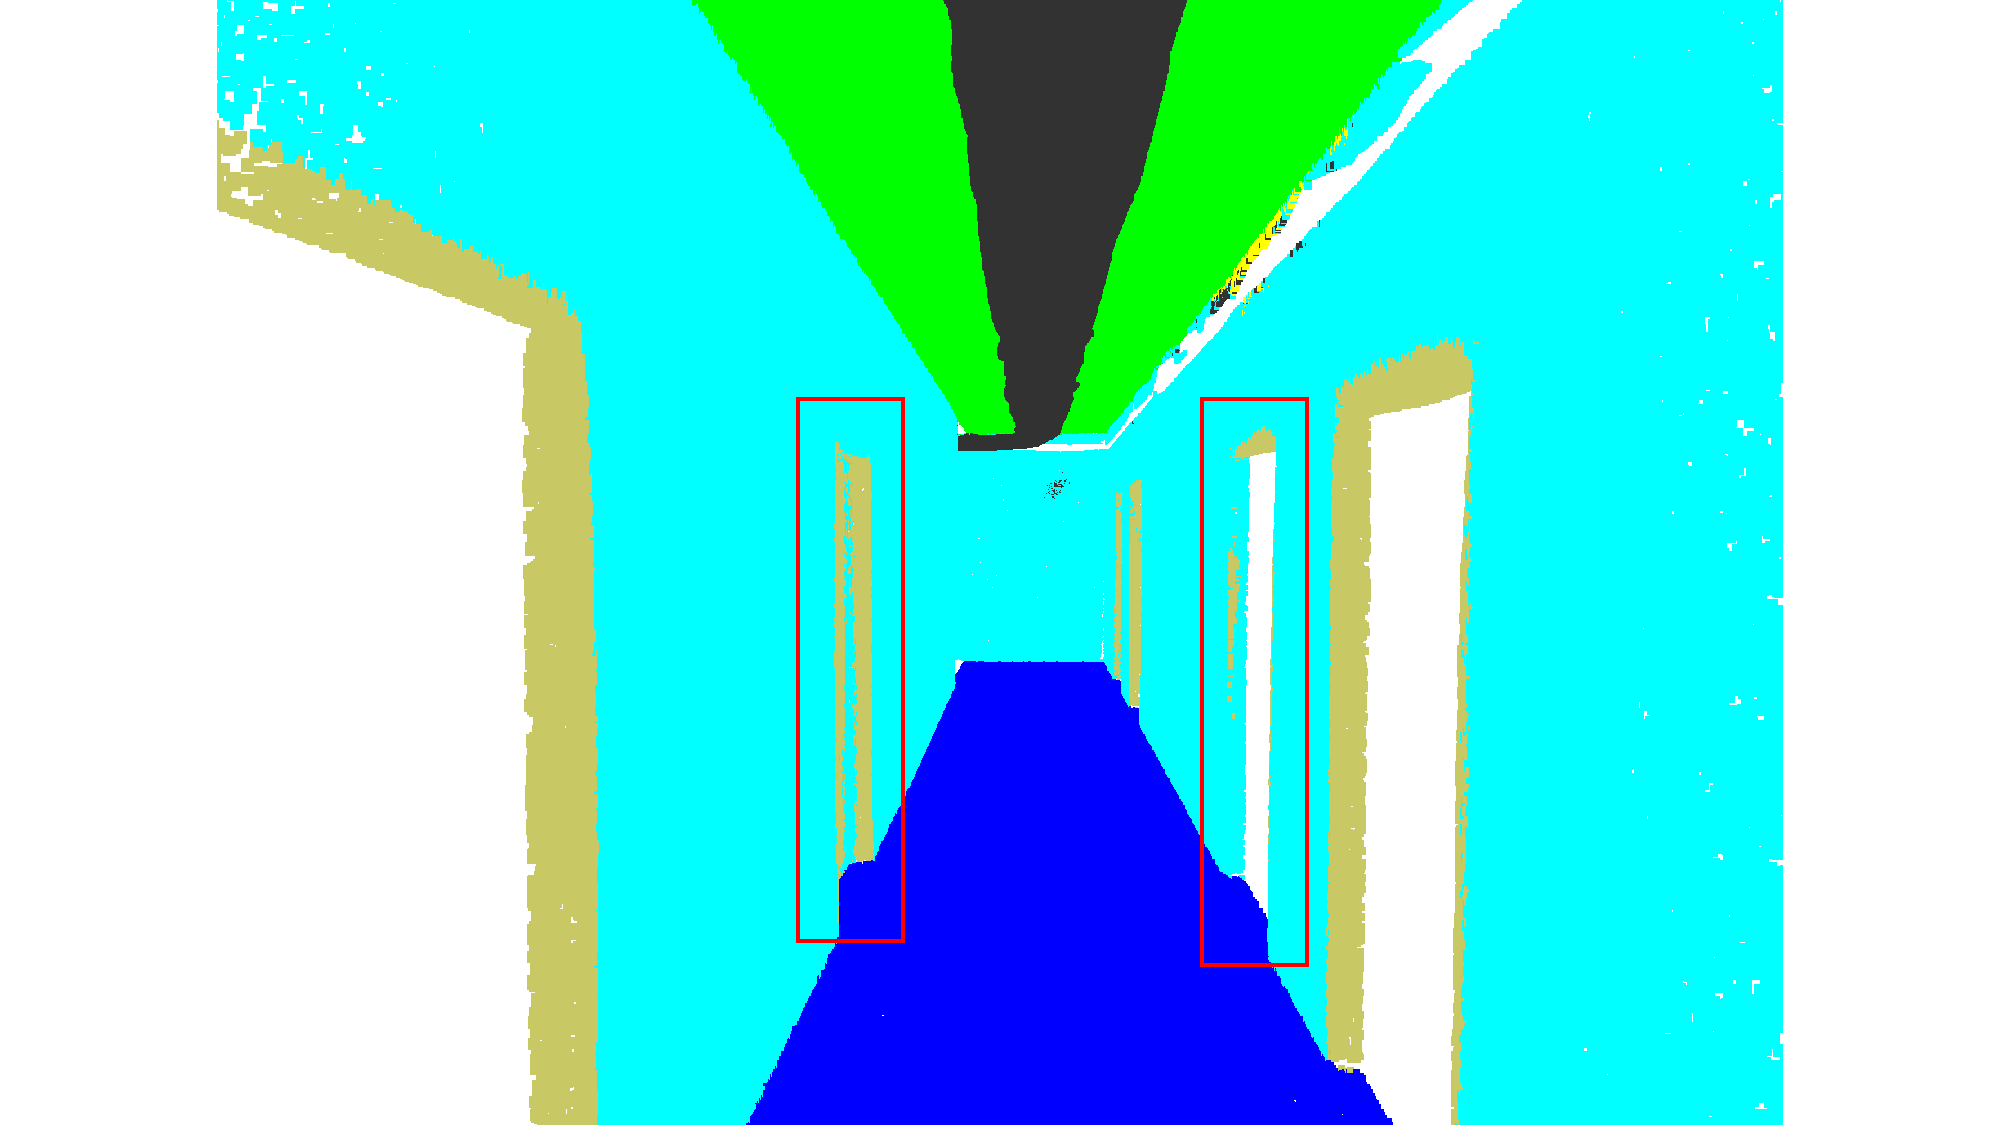
\includegraphics[width=\textwidth]{fig/supplement/semantic_segmentation/hallway_10/PPT_hallway_10.pdf}
    \end{minipage}
    \hfill
    \begin{minipage}{0.22\textwidth}
        \centering
        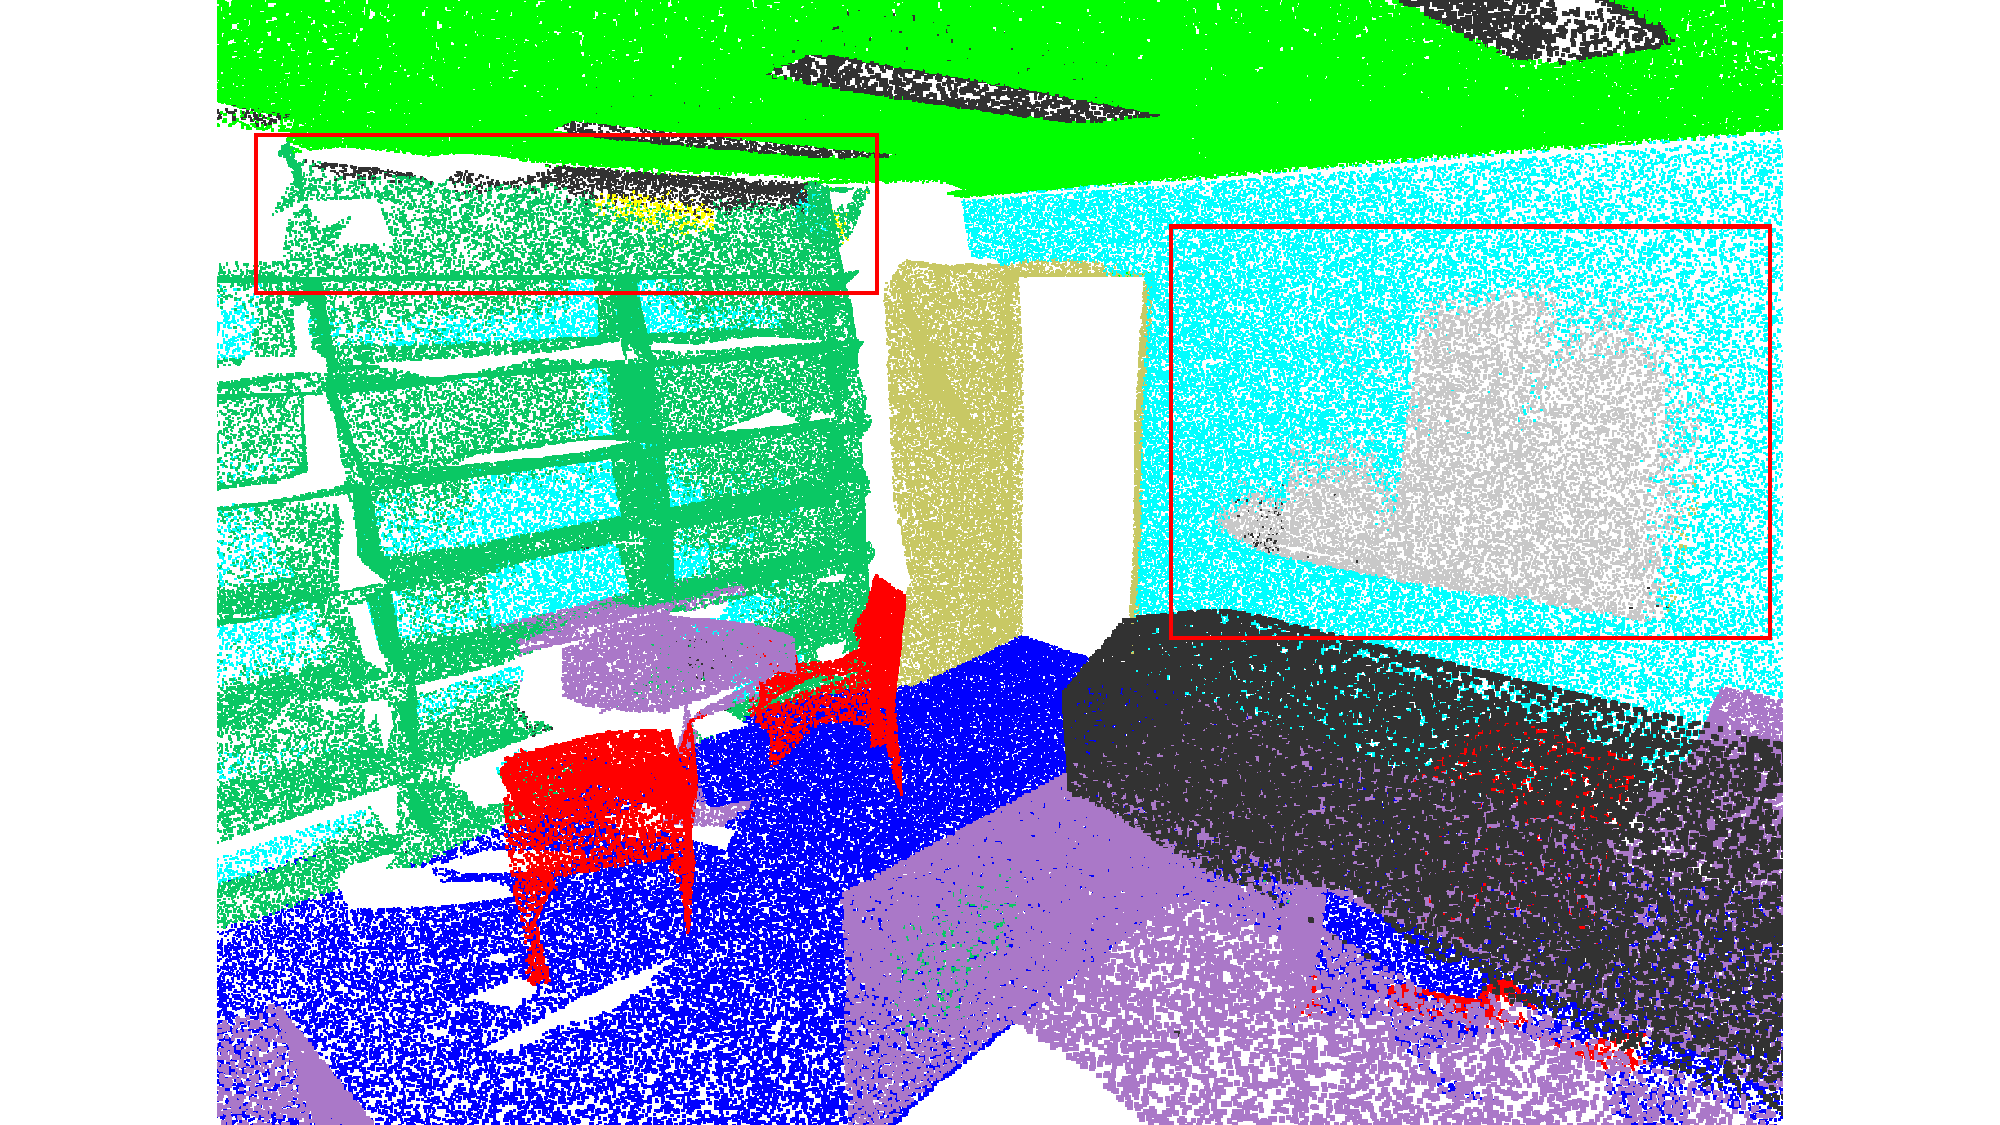
\includegraphics[width=\textwidth]{fig/supplement/semantic_segmentation/office_35/PPT_office_35.pdf}
    \end{minipage}
    \hfill
    \begin{minipage}{0.22\textwidth}
        \centering
        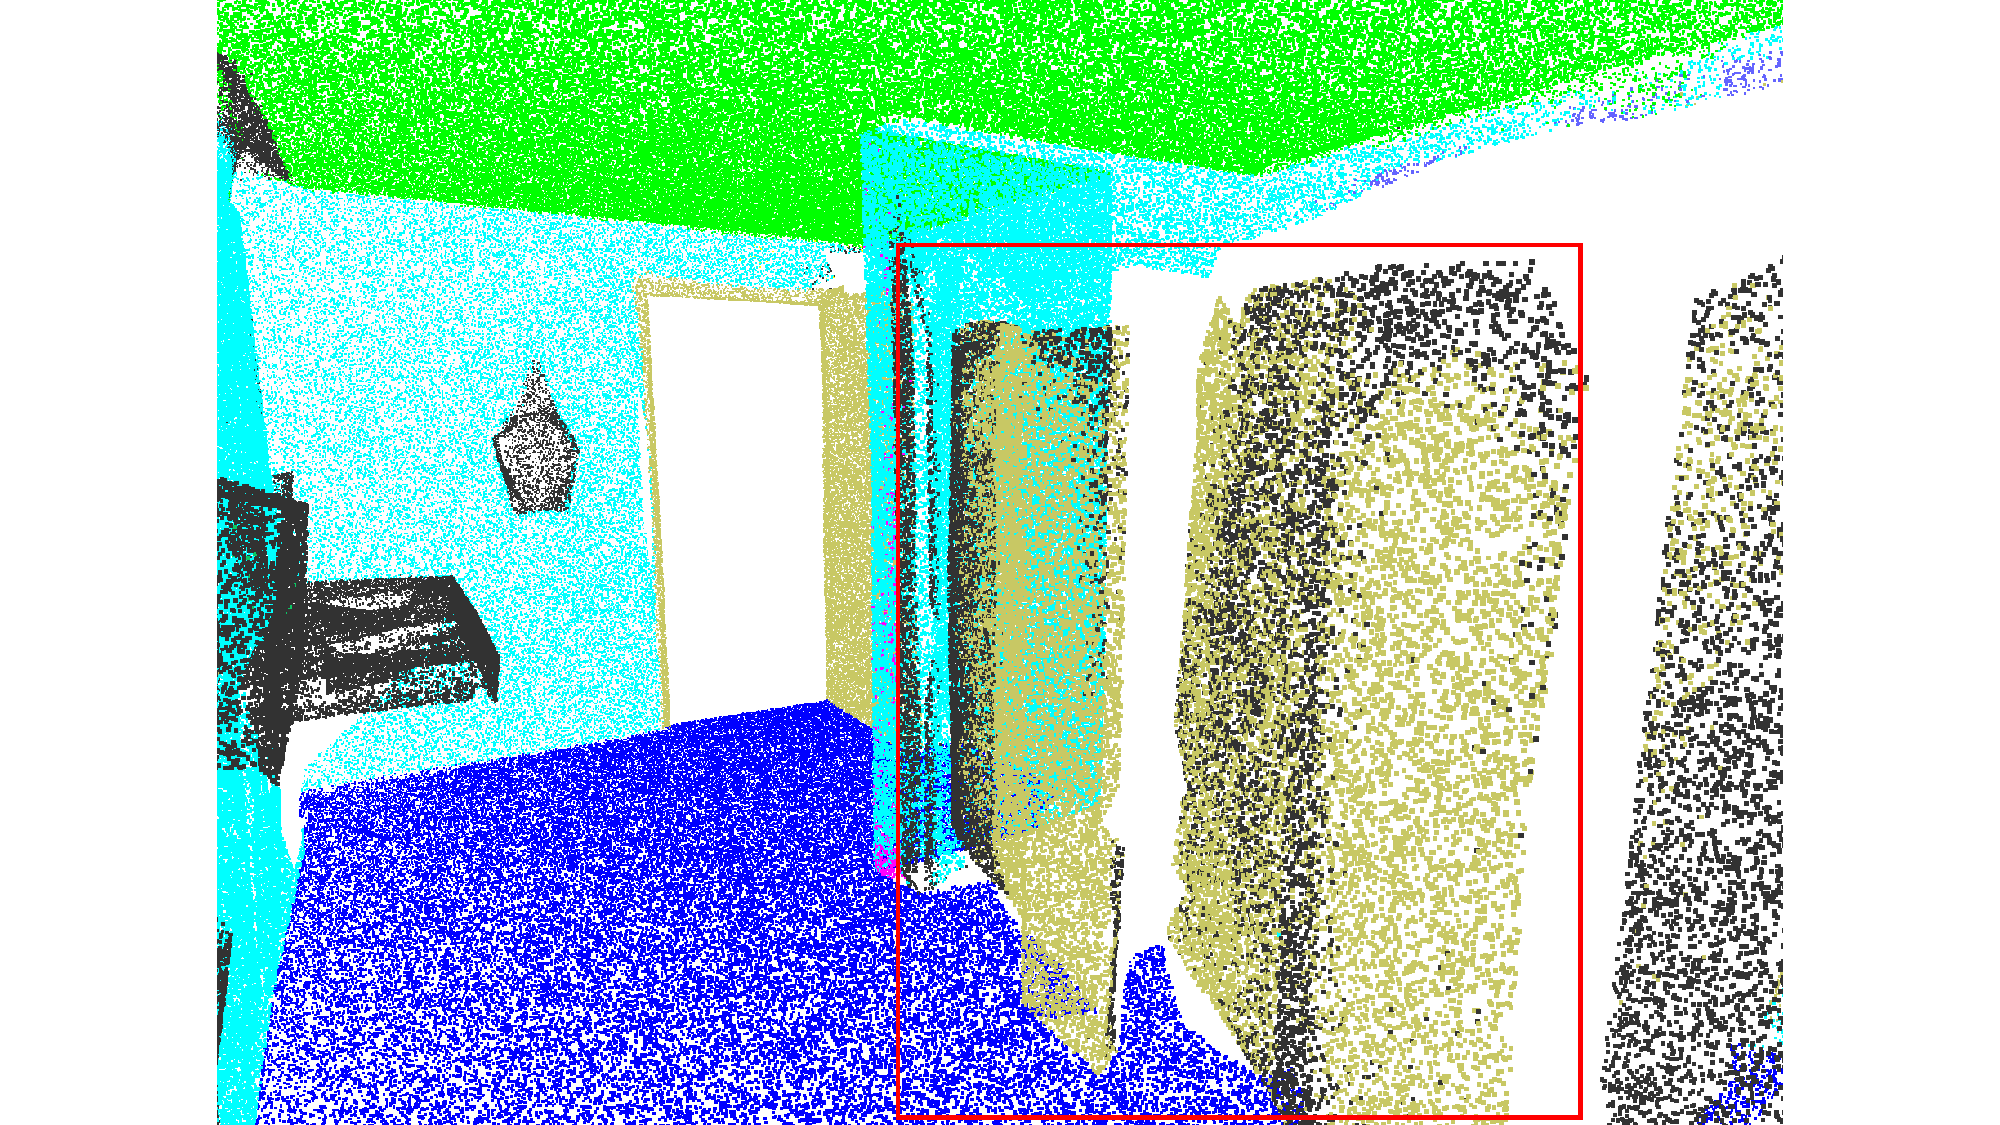
\includegraphics[width=\textwidth]{fig/supplement/semantic_segmentation/wc_2/PPT_wc_2.pdf}
    \end{minipage}
    \hfill

    % 换行
    \vspace{0.5em}

    % 第五行左侧的竖排标签
    \begin{minipage}{0.09\textwidth}
        \centering
        PointGST
    \end{minipage}
    \hfill
    % 第五行图片
    \begin{minipage}{0.22\textwidth}
        \centering
        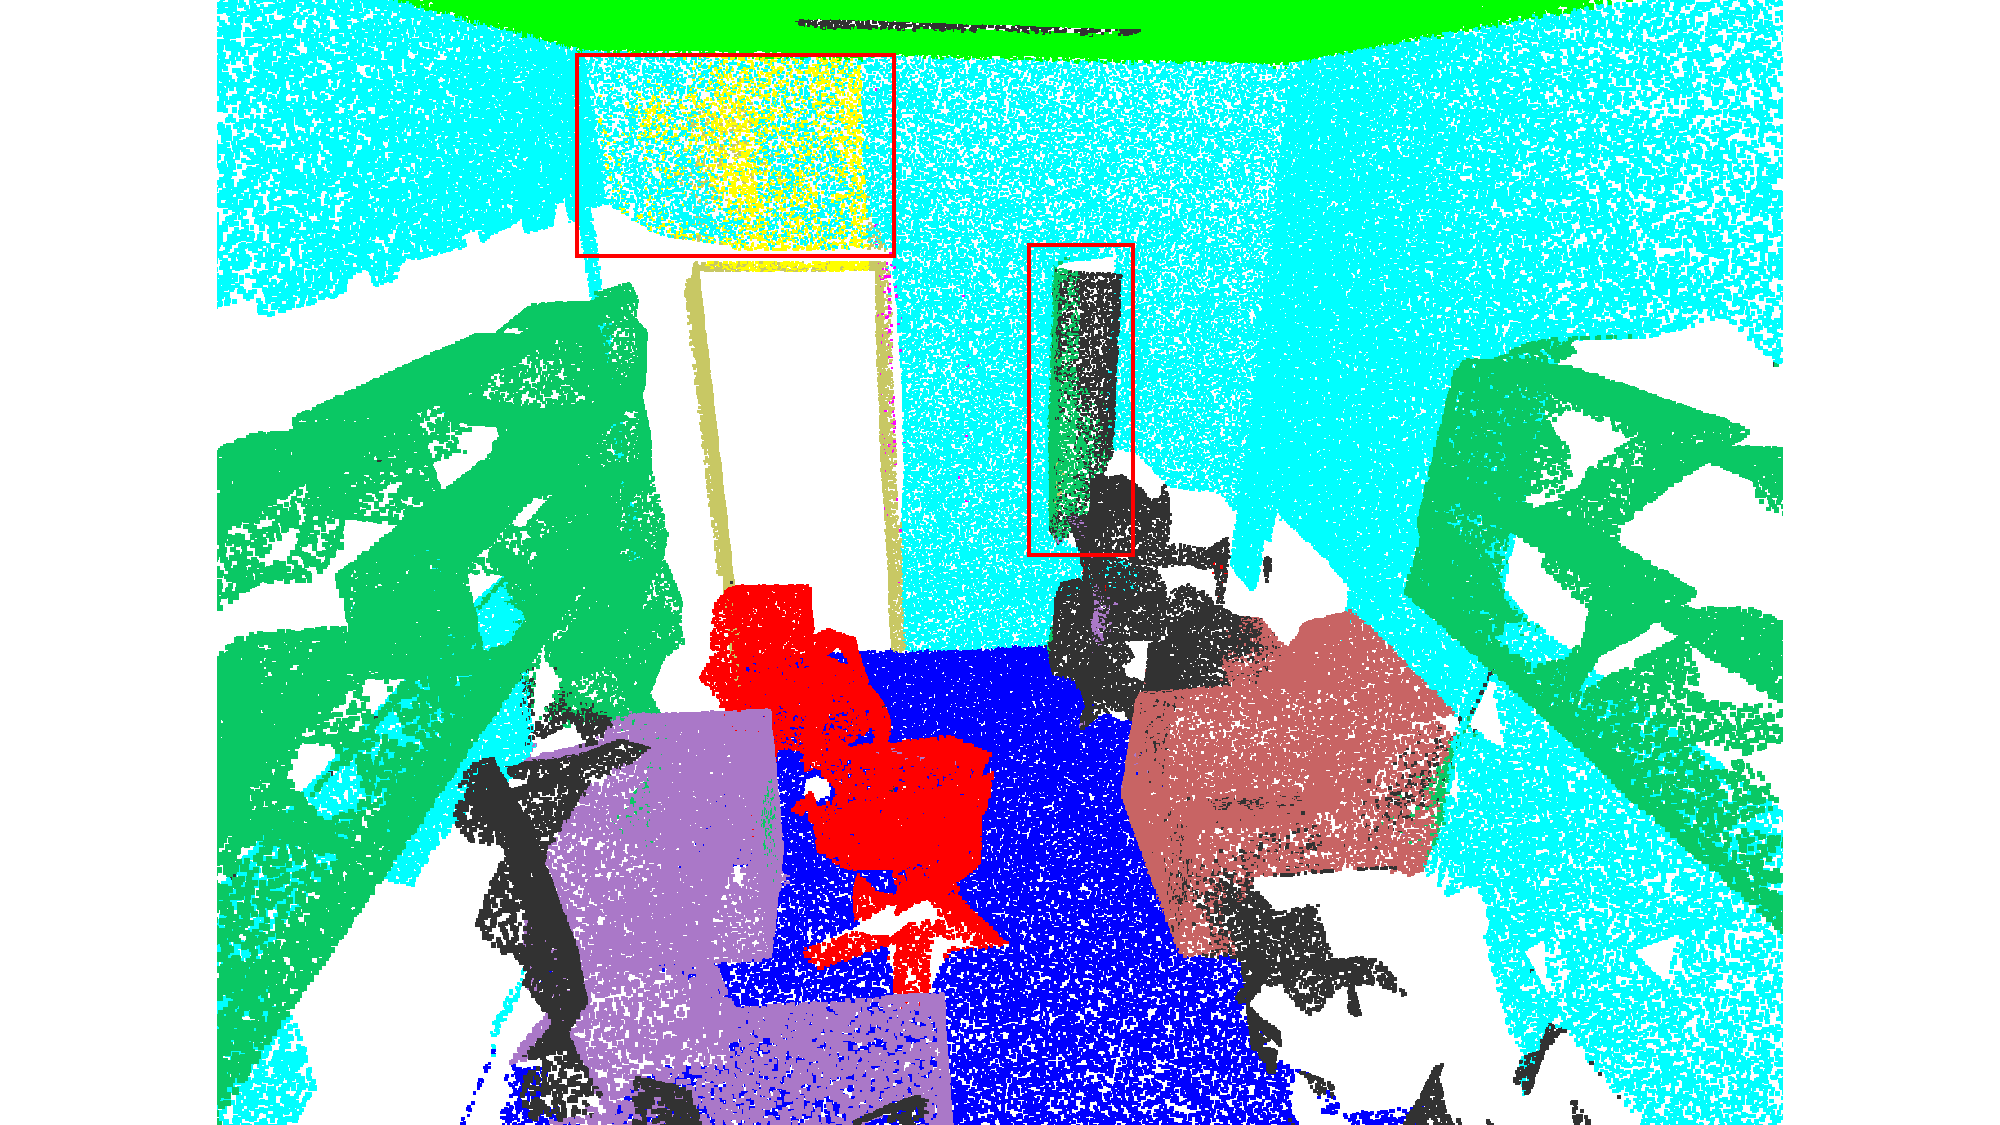
\includegraphics[width=\textwidth]{fig/supplement/semantic_segmentation/office_9/PointGST_office_9.pdf}
    \end{minipage}
    \hfill
    \begin{minipage}{0.22\textwidth}
        \centering
        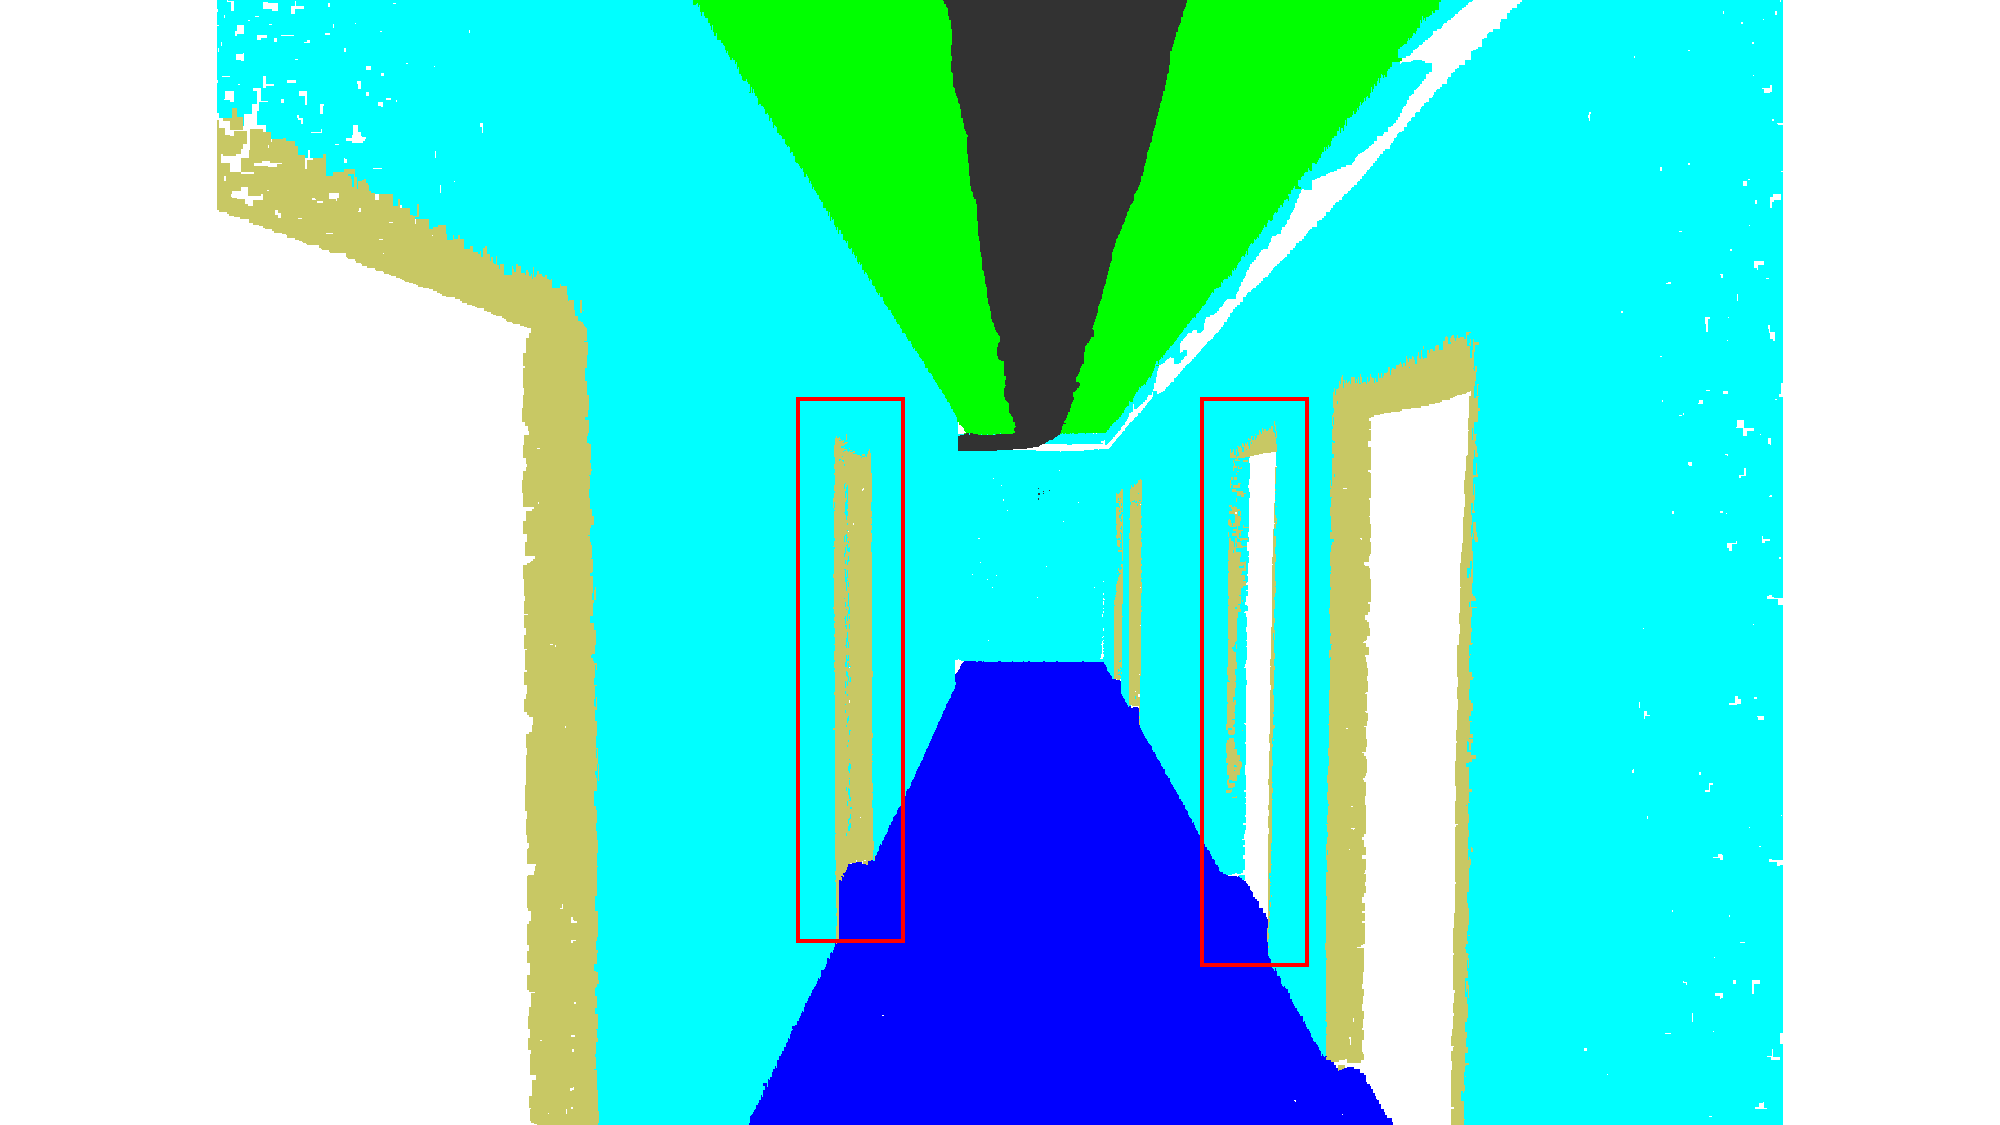
\includegraphics[width=\textwidth]{fig/supplement/semantic_segmentation/hallway_10/PointGST_hallway_10.pdf}
    \end{minipage}
    \hfill
    \begin{minipage}{0.22\textwidth}
        \centering
        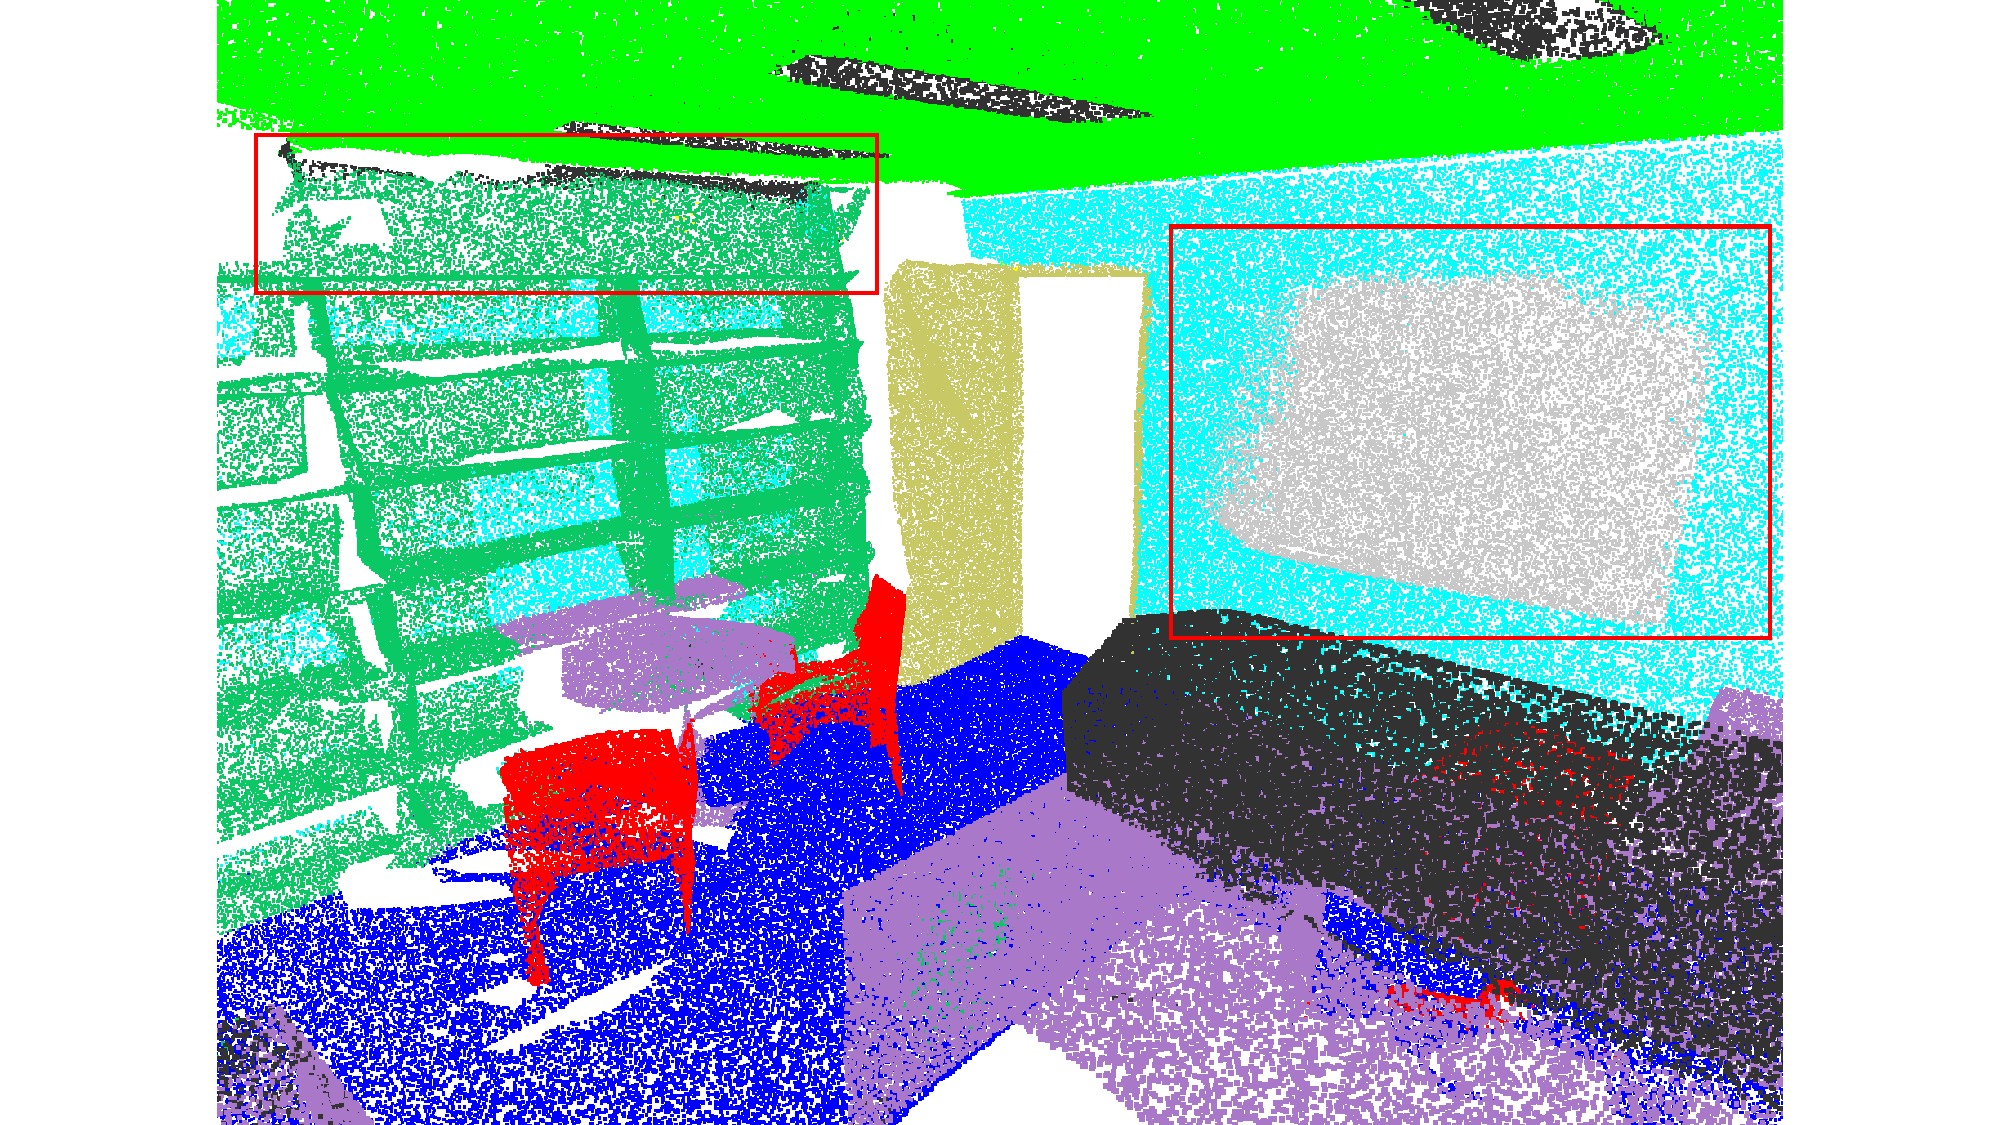
\includegraphics[width=\textwidth]{fig/supplement/semantic_segmentation/office_35/PointGST_office_35.pdf}
    \end{minipage}
    \hfill
    \begin{minipage}{0.22\textwidth}
        \centering
        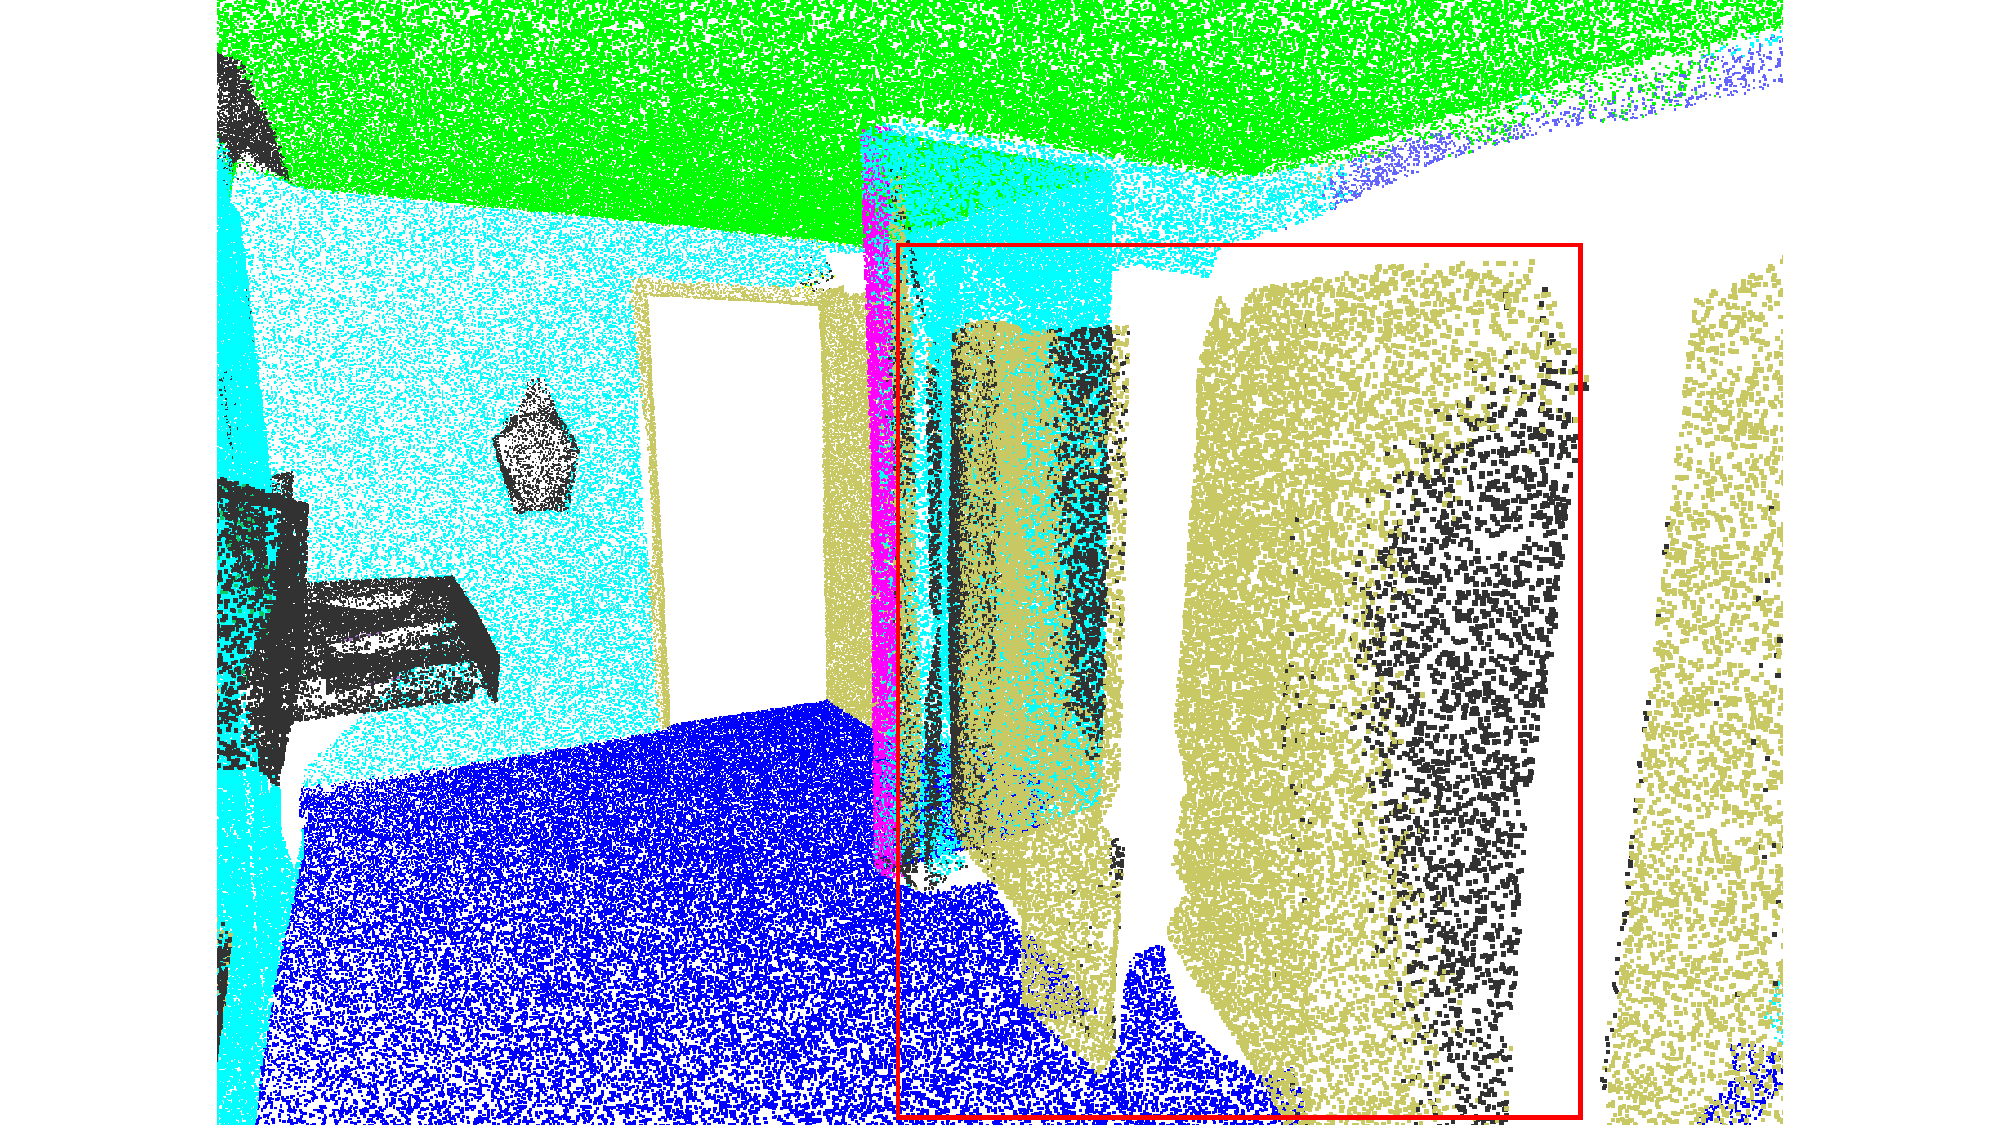
\includegraphics[width=\textwidth]{fig/supplement/semantic_segmentation/wc_2/PointGST_wc_2.pdf}
    \end{minipage}
    \hfill

    % 换行
    \vspace{0.5em}

    % 第六行左侧的竖排标签
    \begin{minipage}{0.09\textwidth}
        \centering
        PLT (Ours)
    \end{minipage}
    \hfill
    % 第六行图片
    \begin{minipage}{0.22\textwidth}
        \centering
        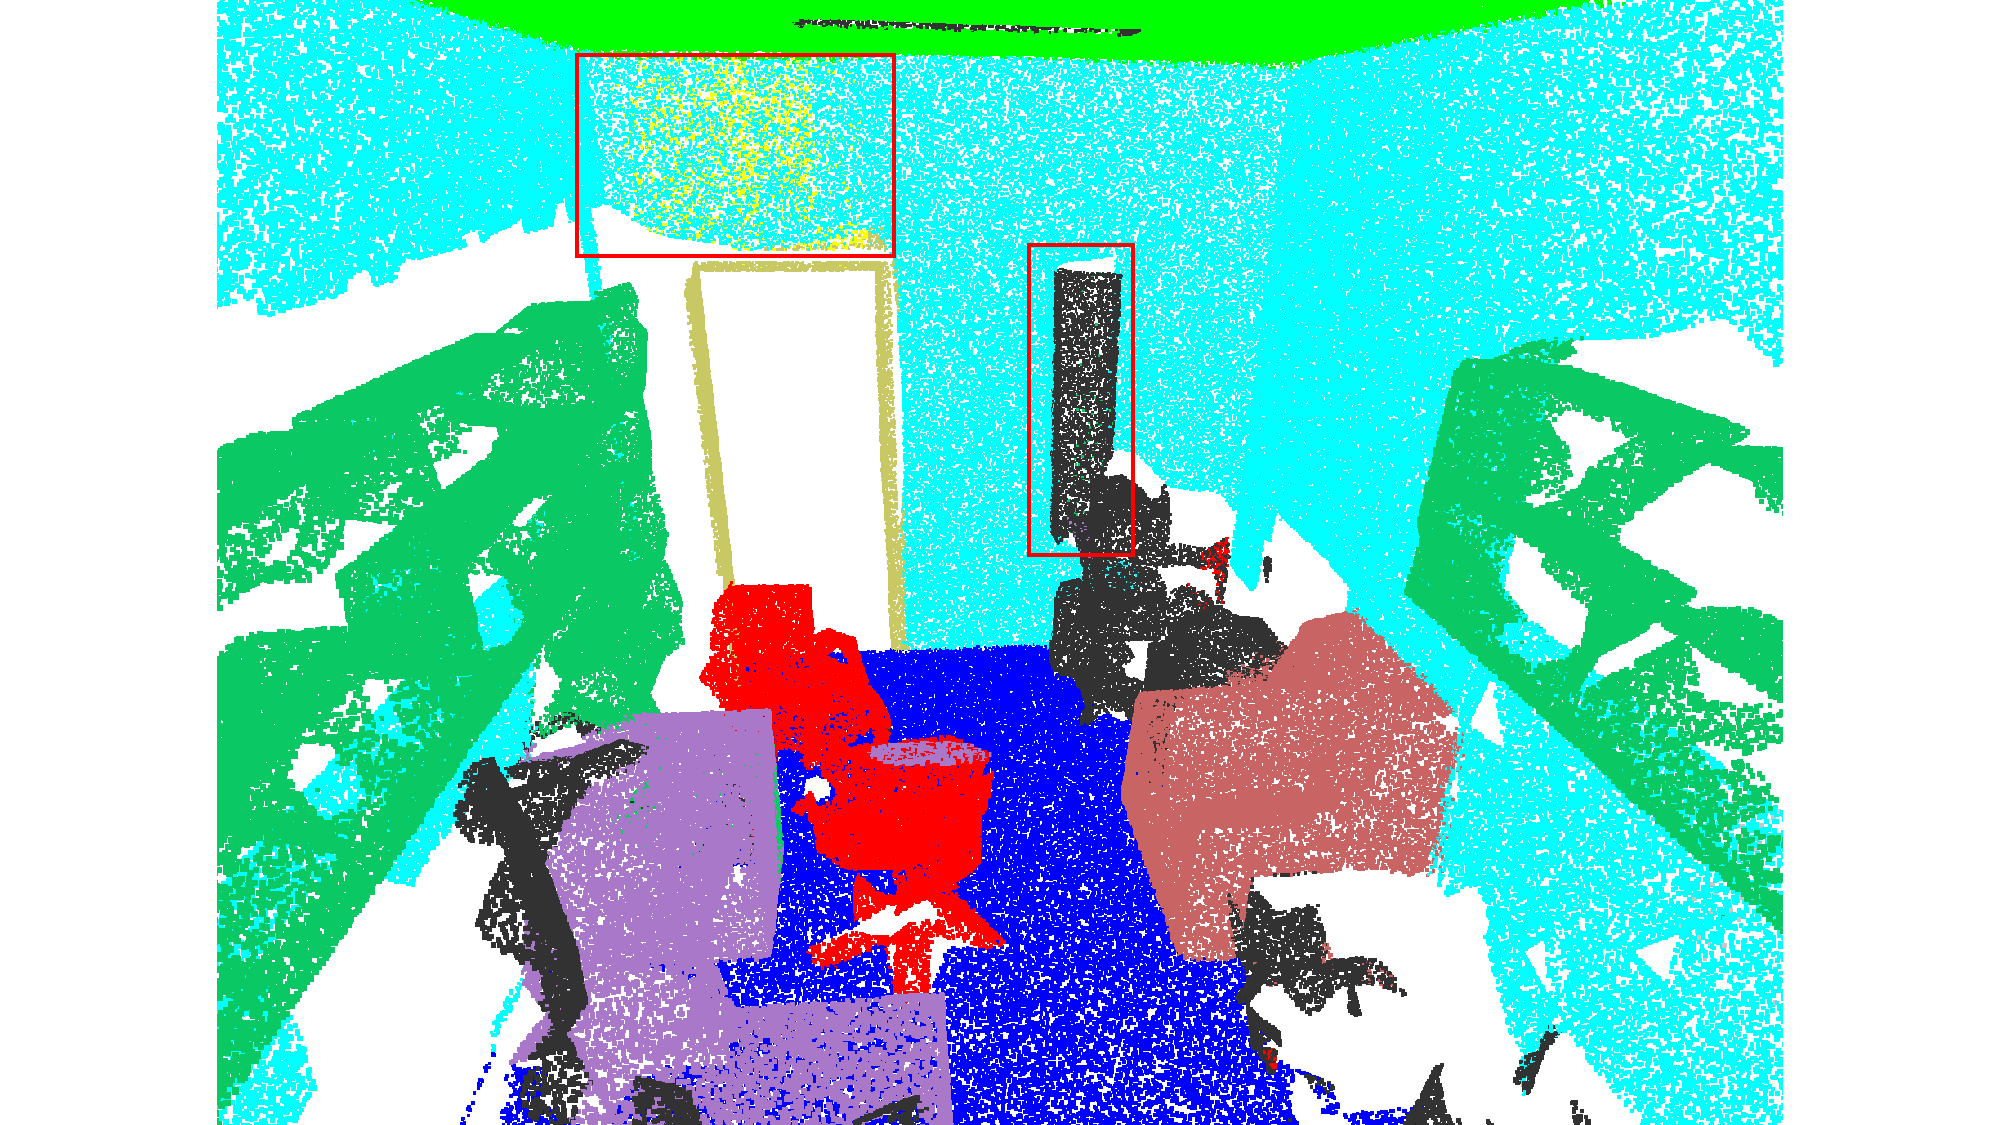
\includegraphics[width=\textwidth]{fig/supplement/semantic_segmentation/office_9/PLT_office_9.pdf}
    \end{minipage}
    \hfill
    \begin{minipage}{0.22\textwidth}
        \centering
        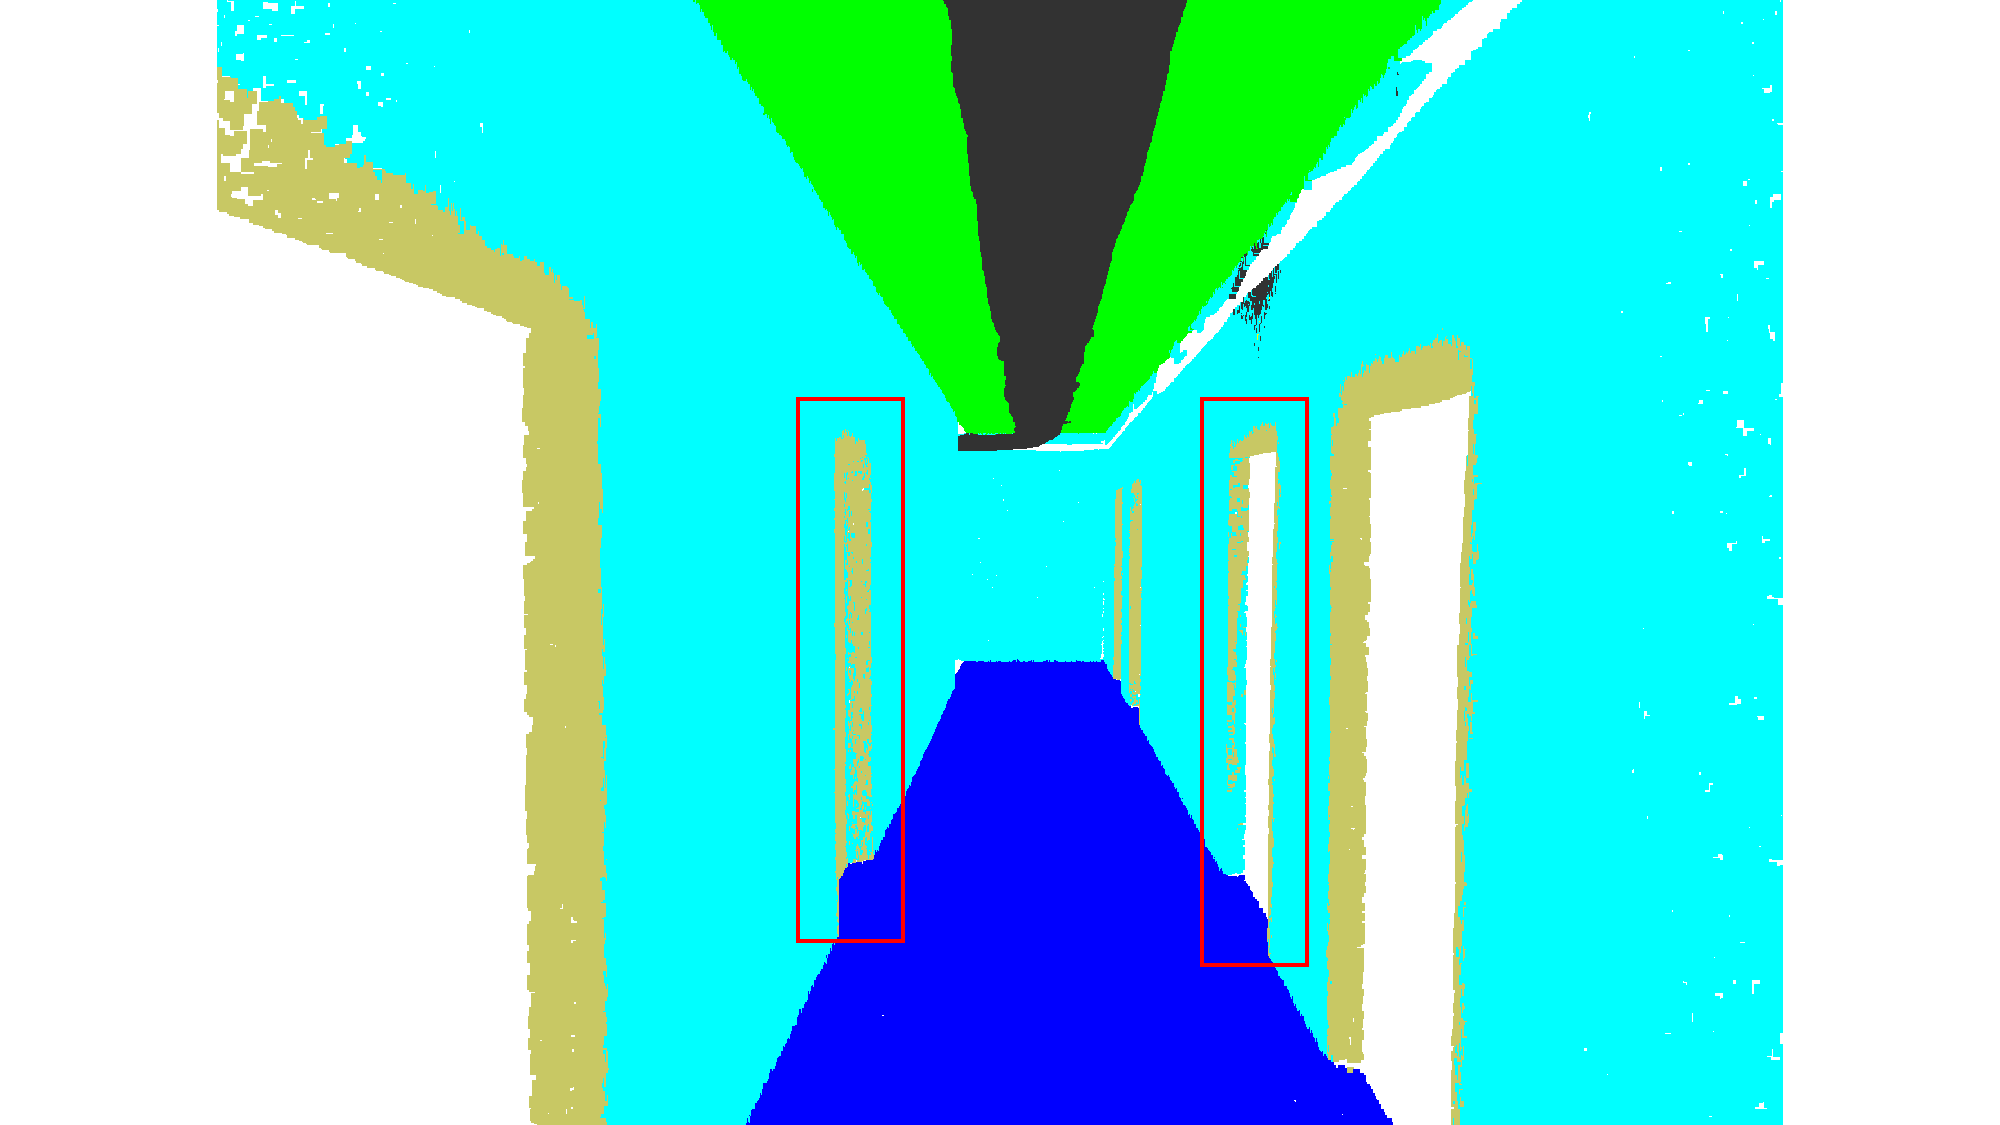
\includegraphics[width=\textwidth]{fig/supplement/semantic_segmentation/hallway_10/PLT_hallway_10.pdf}
    \end{minipage}
    \hfill
    \begin{minipage}{0.22\textwidth}
        \centering
        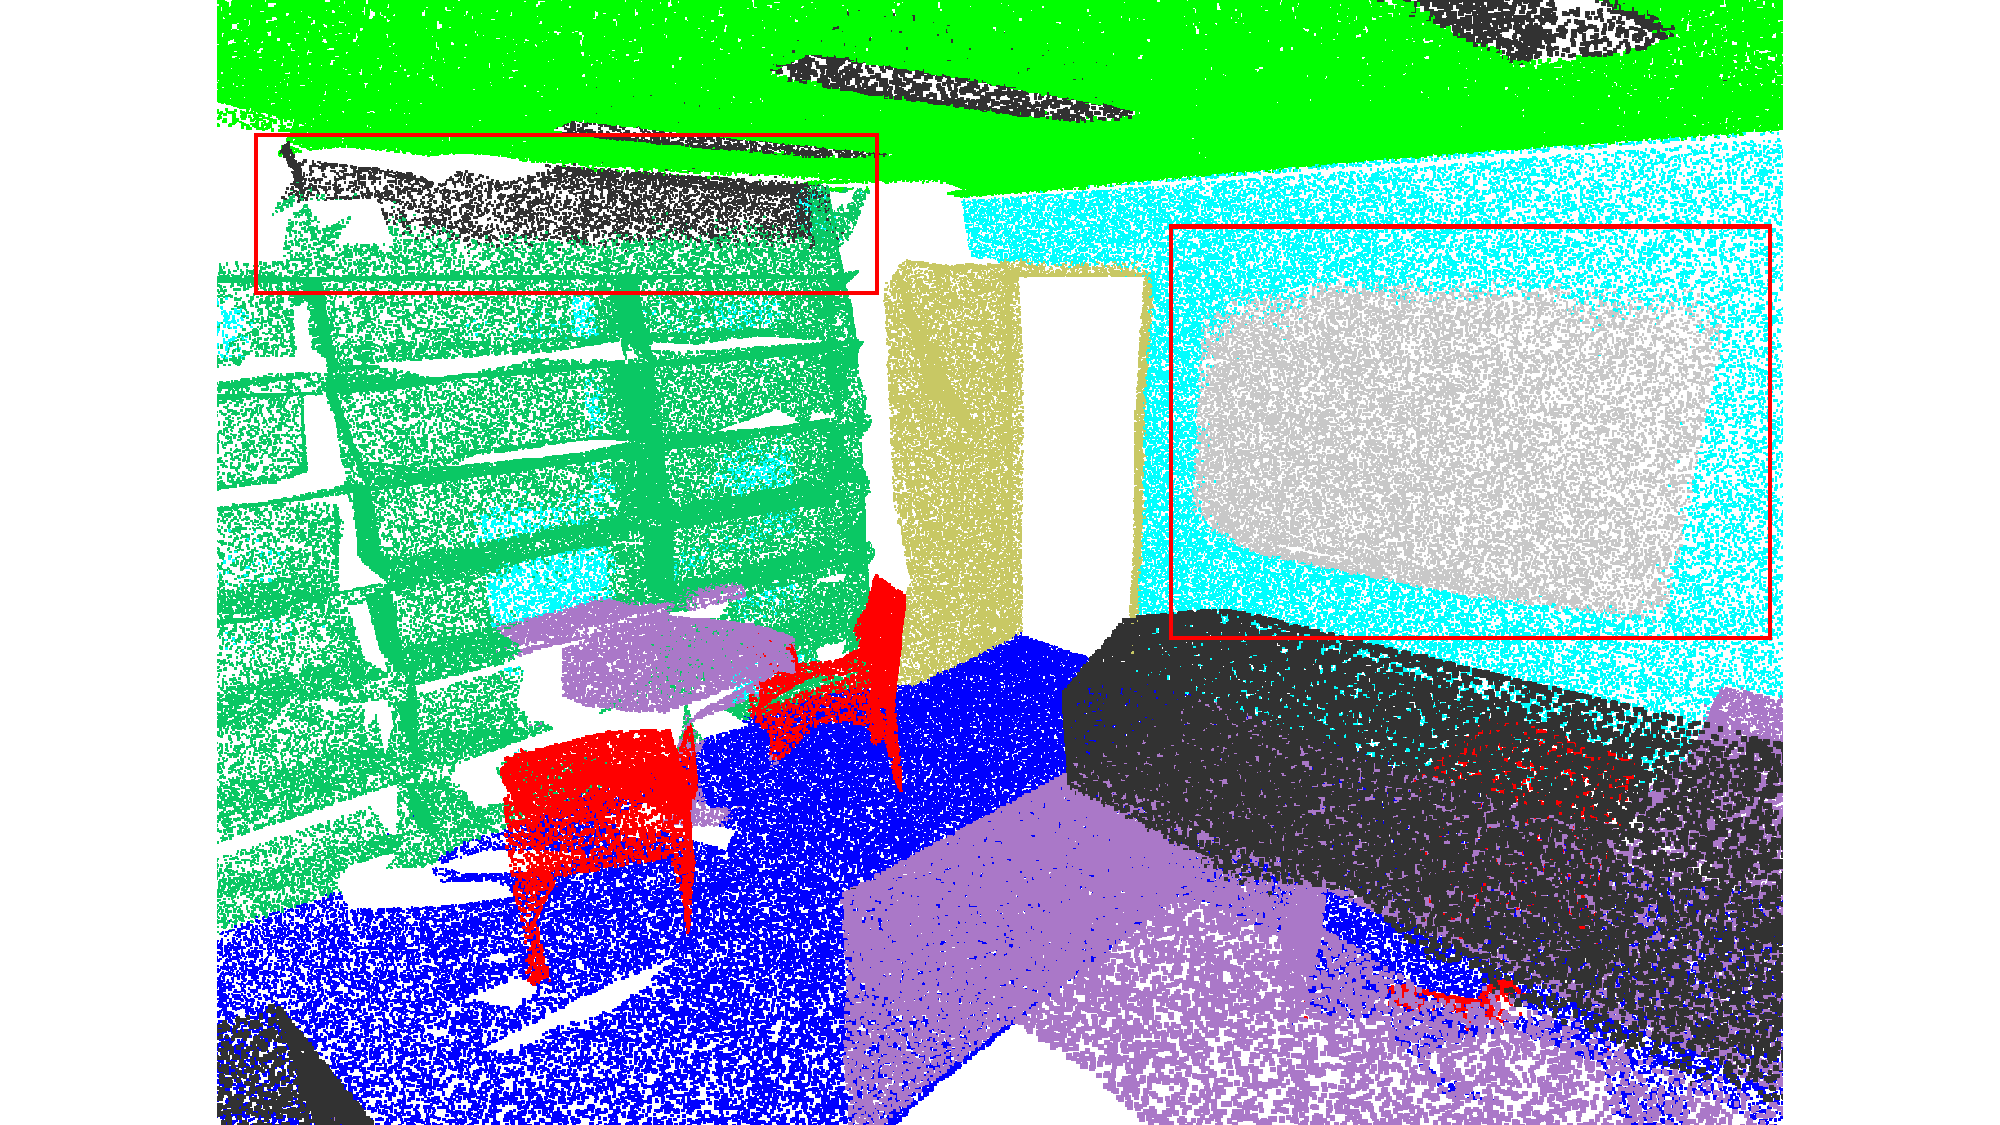
\includegraphics[width=\textwidth]{fig/supplement/semantic_segmentation/office_35/PLT_office_35.pdf}
    \end{minipage}
    \hfill
    \begin{minipage}{0.22\textwidth}
        \centering
        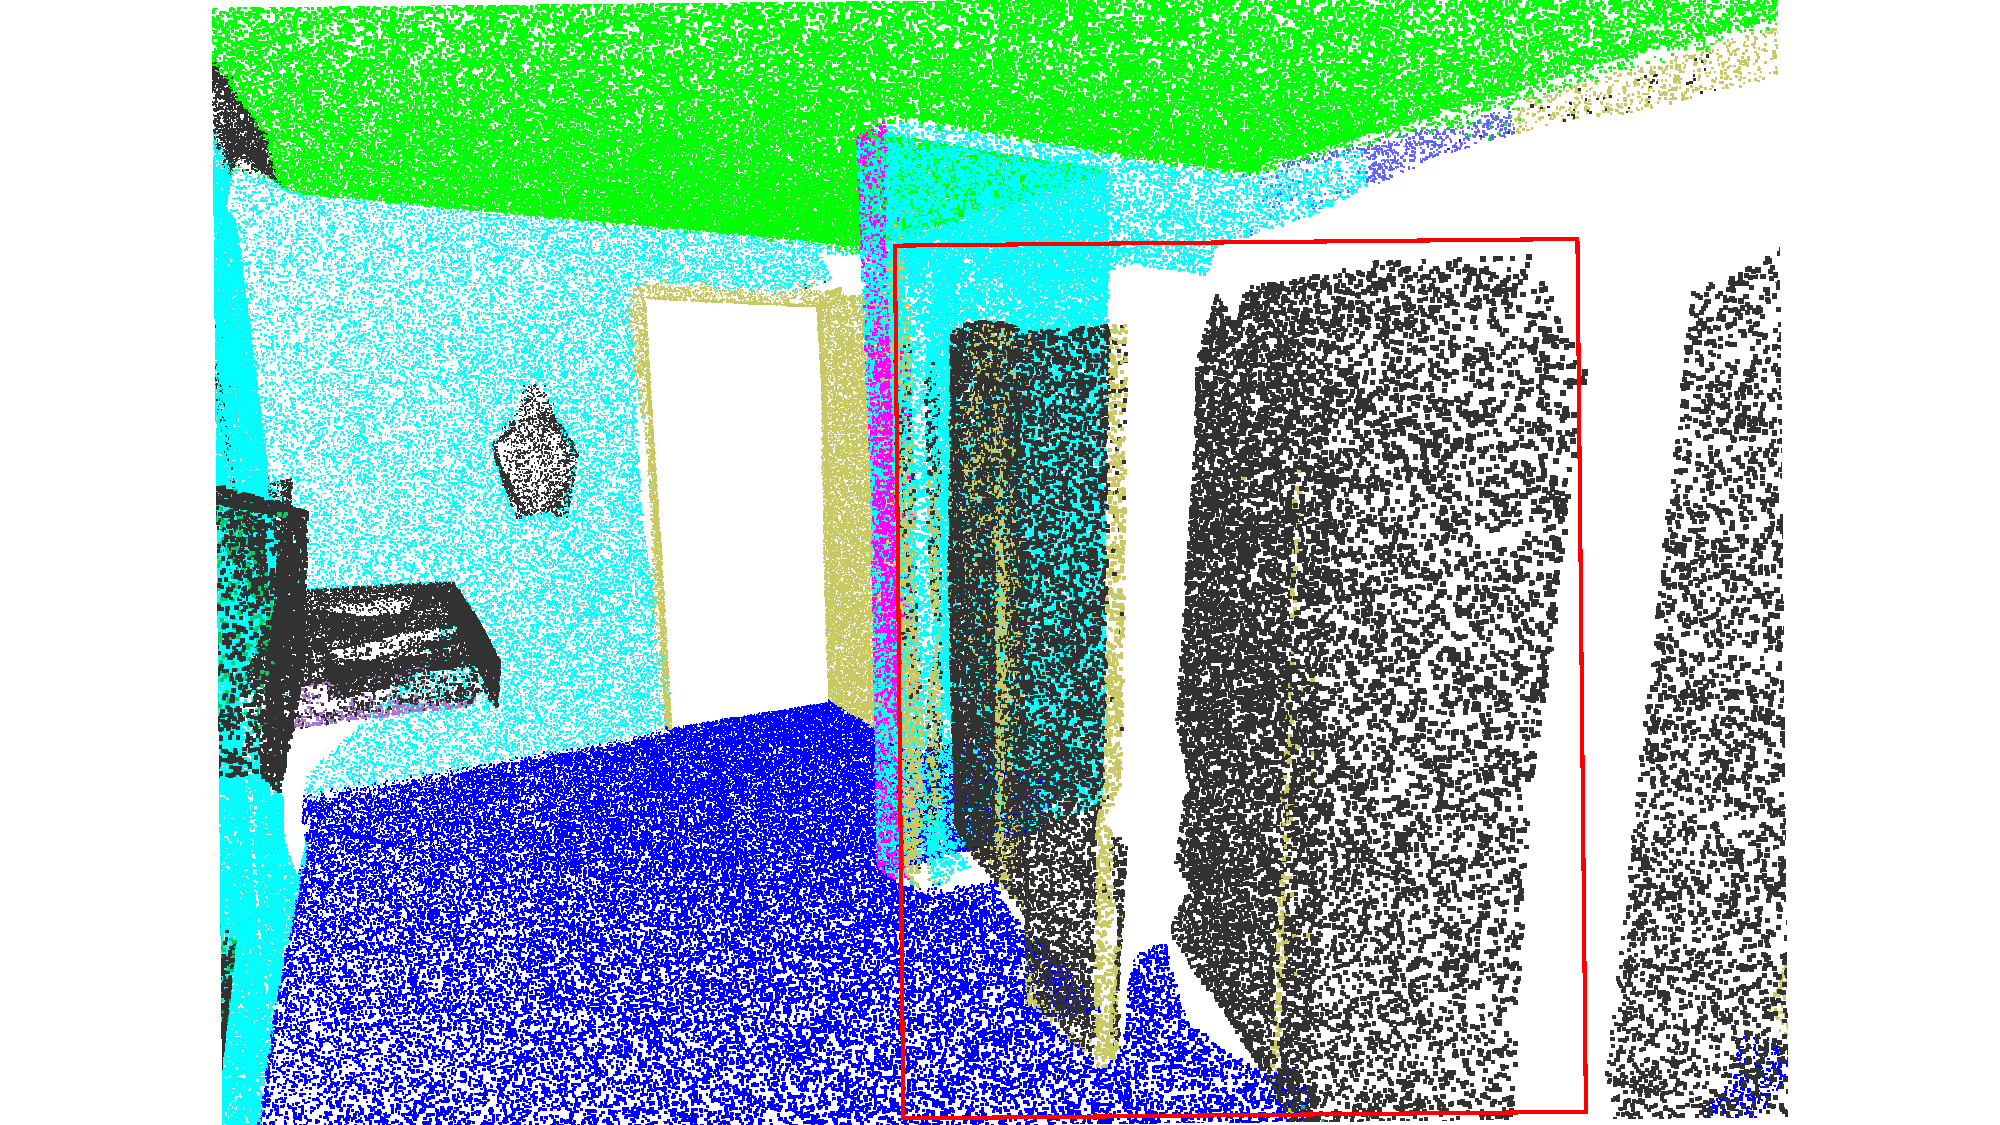
\includegraphics[width=\textwidth]{fig/supplement/semantic_segmentation/wc_2/PLT_wc_2.pdf}
    \end{minipage}
    \hfill

    % 换行
    \vspace{0.5em}

    % 第七行左侧的竖排标签
    \begin{minipage}{0.09\textwidth}
        \centering
        GT
    \end{minipage}
    \hfill
    % 第七行图片
    \begin{minipage}{0.22\textwidth}
        \centering
        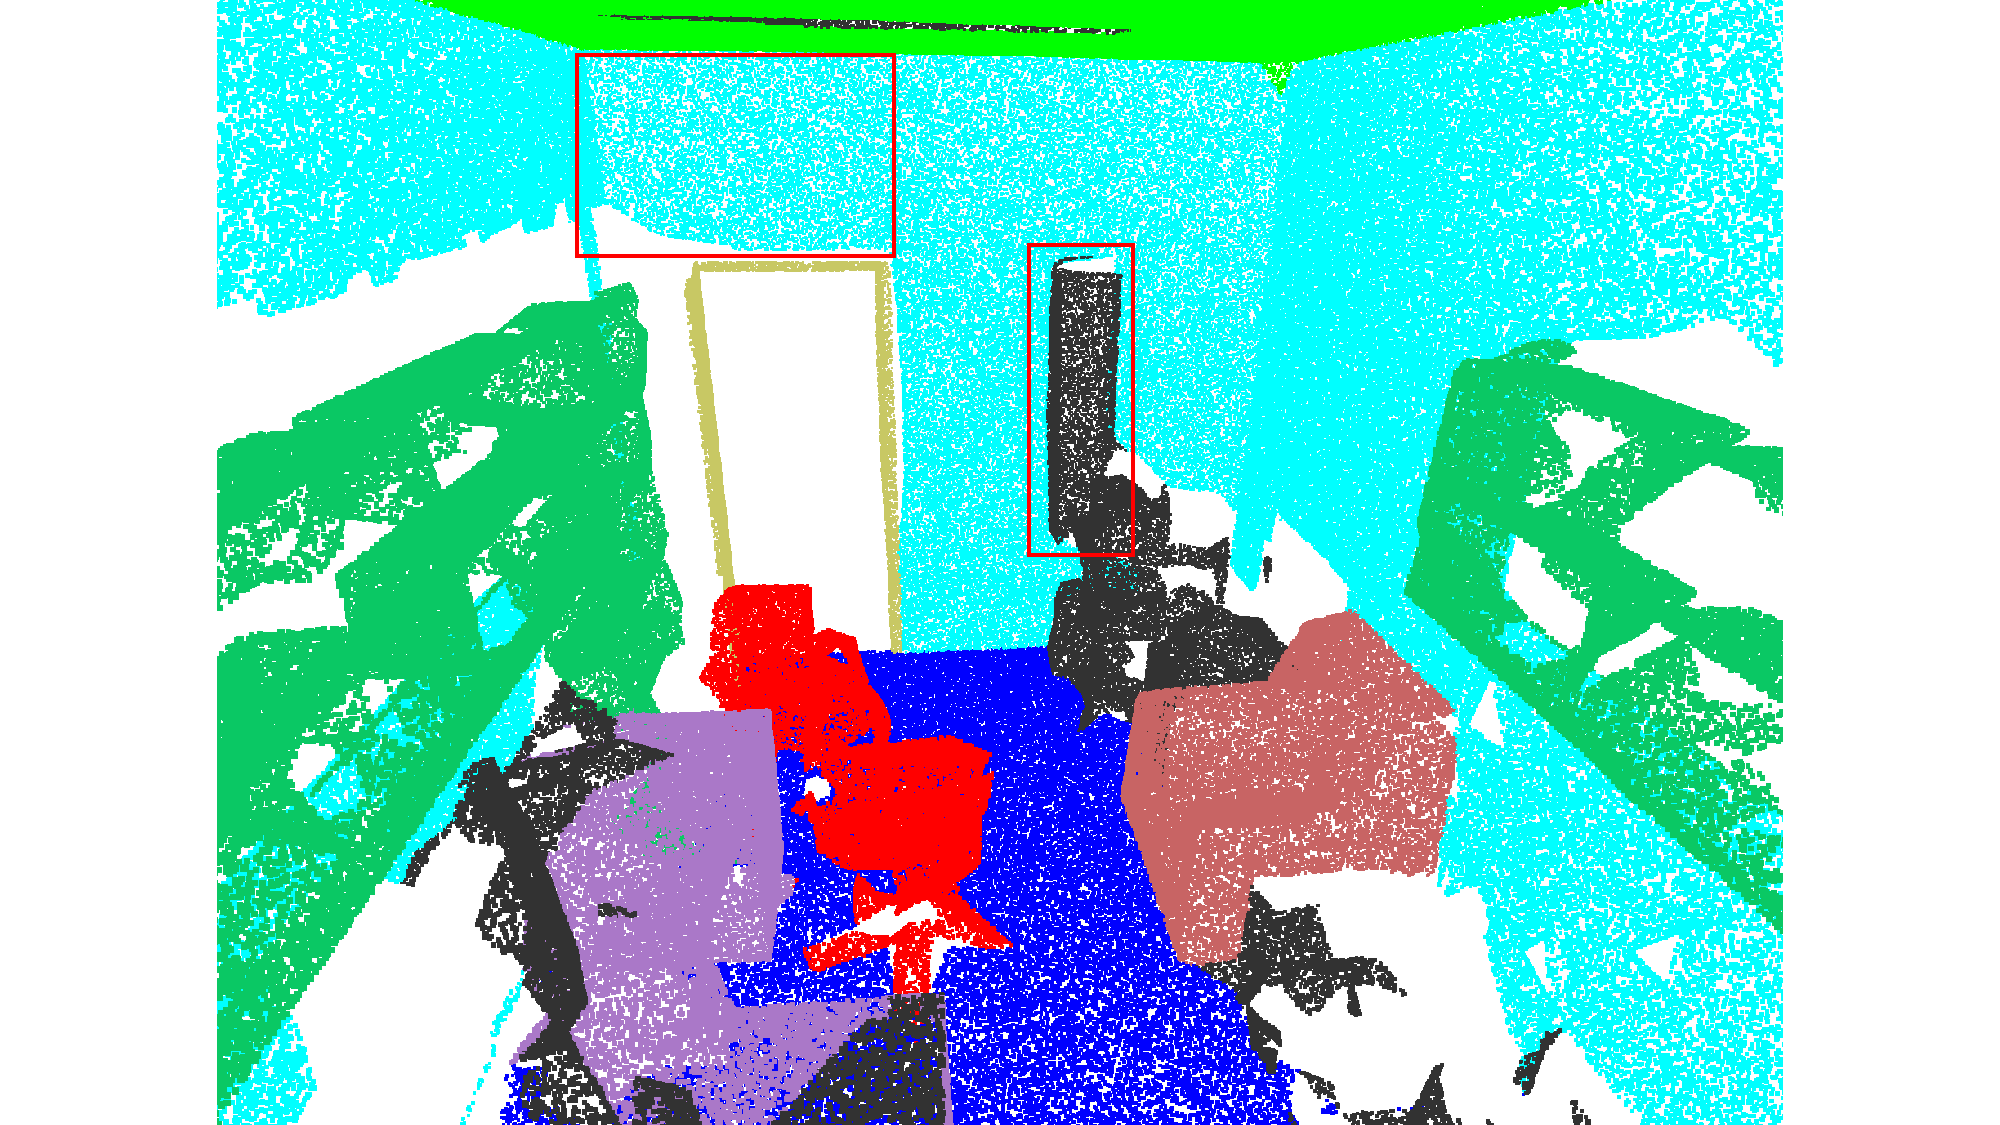
\includegraphics[width=\textwidth]{fig/supplement/semantic_segmentation/office_9/GT_office_9.pdf}
    \end{minipage}
    \hfill
    \begin{minipage}{0.22\textwidth}
        \centering
        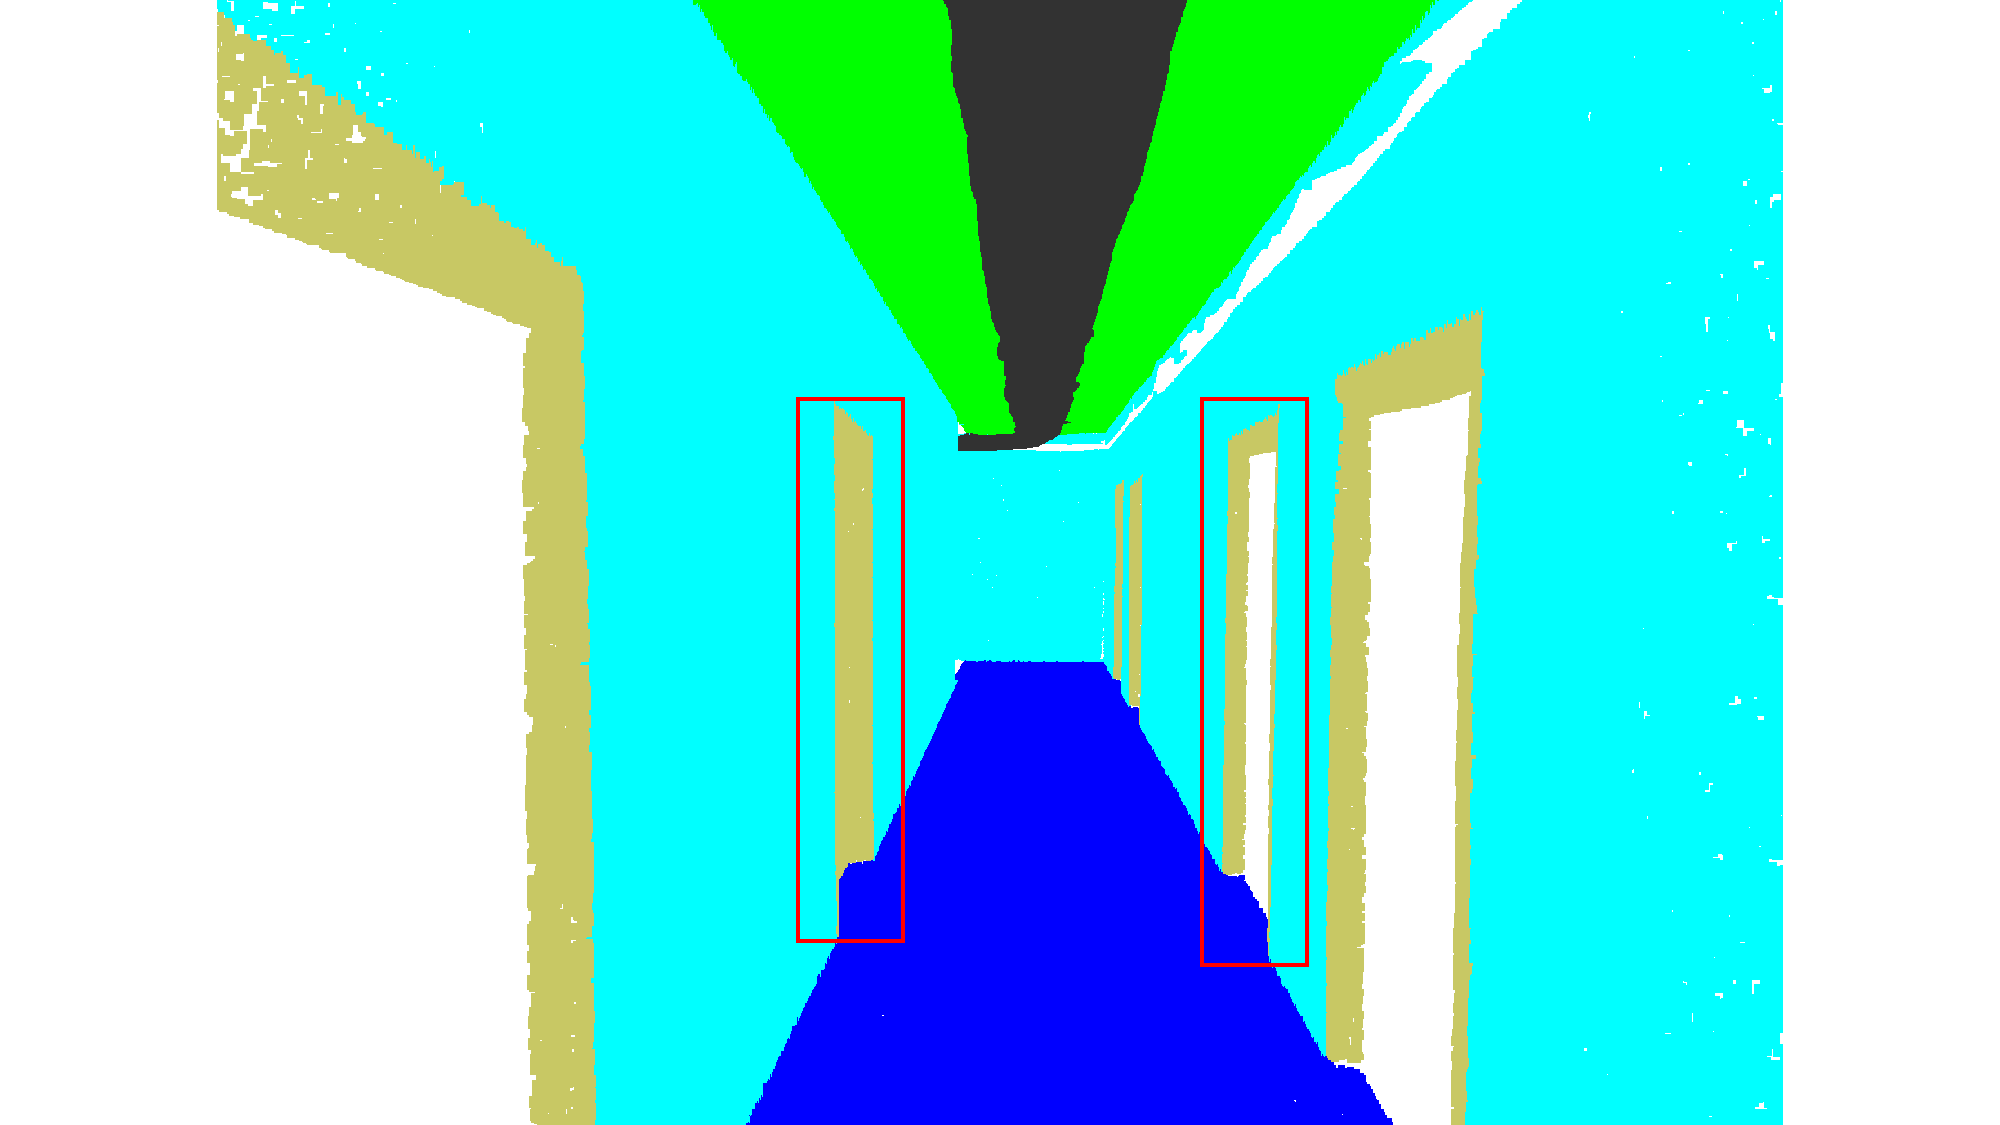
\includegraphics[width=\textwidth]{fig/supplement/semantic_segmentation/hallway_10/GT_hallway_10.pdf}
    \end{minipage}
    \hfill
    \begin{minipage}{0.22\textwidth}
        \centering
        \includegraphics[width=\textwidth]{fig/supplement/semantic_segmentation/office_35/GT_office_35.pdf}
    \end{minipage}
    \hfill
    \begin{minipage}{0.22\textwidth}
        \centering
        \includegraphics[width=\textwidth]{fig/supplement/semantic_segmentation/wc_2/GT_wc_2.pdf}
    \end{minipage}
    \hfill
    
    %下方的标签
    \vspace{0.5em}
    \begin{minipage}{0.09\textwidth} % 左侧空白区域
        \color{white}{12}
    \end{minipage}
    \hfill
    \begin{minipage}{0.22\textwidth} % 第2列标题
        \centering
        office\_9
    \end{minipage}
    \hfill
    \begin{minipage}{0.22\textwidth} % 第1列标题
        \centering
        hallway\_10
    \end{minipage}
    \hfill
    \begin{minipage}{0.22\textwidth} % 第3列标题
        \centering
        office\_35
    \end{minipage}
    \hfill
    \begin{minipage}{0.22\textwidth} % 第3列标题
        \centering
        wc\_2
    \end{minipage}
    \hfill
    \caption{The visualization of qualitative results for point cloud semantic segmentation. We compare our PLT with previous methods on Area 5 of the S3DIS dataset~\cite{armeni20163d}.}
    \label{fig:s3dis_1}

\end{figure*}

